\documentclass[phdthesis,12pt]{wuthesis}

\usepackage{url}
\usepackage{hyperref}
\usepackage{tikz}
\usepackage{float}
\usepackage{graphicx}
\usepackage{cprotect}
\usepackage{amsmath}
\usepackage{longtable}
\usepackage{fancyvrb}
\usepackage{subscript}
\usepackage{hyperref}
\usepackage{fixltx2e}

\usetikzlibrary{shapes, calc, patterns, arrows, decorations.pathreplacing, decorations.markings, positioning, automata}

\newcommand{\rcgo}{rc\textsubscript{go}}

\renewcommand{\thesisauthor}{Justin Wilson}
\renewcommand{\thesisauthorlastname}{Wilson}

\renewcommand{\thesisdepartment}{Department of Computer Science and Engineering}
\renewcommand{\thesisfield}{Computer Science}

\renewcommand{\thesismonth}{December}
\renewcommand{\thesisyear}{2016}

\renewcommand{\thesistitle}{A Transactional Model and Platform for Designing and Implementing Reactive Systems}
\renewcommand{\thesisshorttitle}{Reactive Components}

\renewcommand{\thesissupervisor}{Professor Christopher Gill}
\renewcommand{\thesiscommittee}{Christopher Gill, Chair \\
  Kunal Agrawal \\
  Roger Chamberlain \\
  Ron Cytron \\
  Dave Peters \\
  Gruia-Catalin Roman}

%% Enter the dedication
%% \renewcommand{\thesisdedication}{Dedicated to my parents.}

\begin{document}
\VerbatimFootnotes

\frontmatter
\begin{thesistitlepage}
%\iffalse
\end{thesistitlepage}

\begin{thesiscopyrightpage}
%\iffalse
\end{thesiscopyrightpage}

\begin{singlespace}
\setcounter{page}{2}
\tableofcontents
\listoftables
\listoffigures
\end{singlespace}

\begin{thesisacknowledgments}

\begin{quote}
Blessed be the God and Father of our Lord Jesus Christ, the Father of mercies and God of all comfort  \emph{2 Corinthians 1:3}
\end{quote}

First and foremost, I would like to thank my wife who has been beside me every step of the way.

I am forever grateful for the patience, guidance, and wise counsel of my advisor Dr. Gill.

The seed for this dissertation was planted by Dr. Roman in the basement of Lopata Hall during a course on UNITY.
He was lecturing on the development of structured programming and the give and take between formal methods and practice.
I am grateful to Dr. Roman for introducing me to the clarity of thinking that comes from formal models.

I would like to thank the Department of Computer Science and Engineering, the National Science Foundation, and the Ford Motor Company for their generous financial support.

\end{thesisacknowledgments}

%% \begin{thesisdedicationpage}                %% Generate the dedication page.
%% %\iffalse
%% \textbf{Note:} You may include a special dedication as shown here.  If you
%% include this page, be sure to keep it brief and center it on the page both
%% horizontally and vertically.  Alternatively, you may remove this page
%% altogether, and a special dedication can be placed as the final paragraph to
%% your acknowledgments page (as shown in this document on the preceding page).
%% %\fi
%% \end{thesisdedicationpage}

\begin{thesisabstract}
\input abstract.tex
\end{thesisabstract}

\mainmatter
\chapter{Introduction}
\label{introduction}

\paragraph{Definitions.}
Manna and Pnueli classify programs as either being \emph{transformational} or \emph{reactive}~\cite{manna1992temporal}.
As implied by their name, transformational programs transform a finite input sequence into a finite output sequence.
Transformational programs often can be divided into three distinct phases corresponding to the activities of input, processing, and output.
A compiler is an example of a transformational program as it transforms a source file into an object file.
Formal models of computation like the Turing machine~\cite{turing1936computable} and $\lambda$-calculus~\cite{church1936unsolvable} are concerned with transformational programs.

In contrast, a reactive program is characterized by ``ongoing interactions with its environment\cite{manna1992temporal}.''
Whereas transformational programs are designed to halt and produce an output (when possible, i.e., the halting problem), reactive programs are often designed to run forever.
The activities of input, processing, and output are thus overlapped in the execution of a reactive program.
A web server is a example of a reactive program as it continually receives requests, processes them, and sends responses.
Reactive systems include operating systems, databases, networked applications, interactive applications, and embedded systems.
A number of formal models have been developed to reason about reactive systems and include the Calculus of Communicating Systems~\cite{milner1982calculus}, the Algebra of Communicating Processes~\cite{bergstra1982fixed}, Cooperating Sequential Processes~\cite{dijkstra1965cooperating}, Communicating Sequential Processes~\cite{hoare1978communicating}, the Actor Model~\cite{hewitt1973universal}\cite{clinger1981foundations}\cite{agha1985actors}, UNITY~\cite{chandy1989parallel}, and I/O automata~\cite{nancy1996distributed}.
A reactive program must share resources with its environment to facilitate communication.
From the perspective of the reactive program, input occurs when the environment acts on the reactive program and output occurs when the reactive program acts on the environment.
The manipulation of resources internal to a reactive program or an environment is generically referred to as processing.

Asynchronous concurrency is a fundamental characteristic of reactive systems that makes them difficult to design and develop.
Concurrency refers to the idea that a reactive program and its environment may act at the same time.
In synchronous models, a reactive program and its environment share a common clock which allows the reactive program to coordinate access to shared resources, e.g., the environment writes a shared variable in one clock cycle and the reactive program reads it in the next.
However, shared clocks are difficult to implement and do not scale.
Consequently, many reactive systems are asynchronous meaning that the reactive program and environment evolve independently with respect to time.
To facilitate communicate, asynchronous models include facilities for atomicity that allow a reactive program to act without being interrupted by its environment and vice versa.
The facilities for atomicity allow a reactive program to synchronize with its environment as the atomic events play the role of a shared clock.
A common approach to ensuring correctness in asynchronous models is to view the environment as an adversary that will deliver inputs at inopportune times.
Since a reactive program may run forever, the designers of reactive programs thus must often reason about infinite event sequences containing interleaved input, output, and processing.

Failure to account for asynchronous concurrency may result in a reactive program with \emph{timing bugs}, meaning that correct execution depends on arbitrary scheduling decisions.
Timing bugs may be manifested when the schedule of events is perturbed, e.g., due to a new processor or operating system, or when part of the program takes more or less time than normal.
Operating systems are particularly susceptible to timing bugs caused by device drivers~\cite{ryzhyk2009dingo}.
Timing bugs can escape even a rigorous software development process and lay dormant for years~\cite{lee2006problem}.
Furthermore, timing bugs are notoriously difficult to diagnose, inspiring the term \emph{heisenbug}, a bug that disappears or changes its behavior when someone is attempting to find it (because the debugging process alters the timing of the program)~\cite{1983proceedings}.
Timing bugs can cost many hours of debugging time and can lead to a poor user experience, e.g., a non-responsive device or application, and loss of revenue, e.g., when an advertisement service cannot be used while a server reboots.

\emph{Decomposition} and \emph{composition} are essential techniques when designing, implementing, and understanding complex systems.
Decomposition, dividing a complex system into a number of simpler systems, is often used when \emph{designing} a system, e.g., through top-down design~\cite{wirth1971program}.
Composition, building a complex system from a number of simpler systems, is often used when \emph{implementing} a system; i.e., simpler systems are implemented, tested, and integrated to create larger systems~\cite{brooks1995mythical}.
Often, the simplest systems in a design are common and can be reused across problem domains.
Similarly, systems in the same problem domain often have common sub-systems.
Thus, a common goal in software engineering is fostering design processes that produce and leverage reusable components.
Decomposition also often imparts a logical organization to a system when the resulting sub-systems are cohesive, i.e., each sub-system has a well-defined purpose~\cite{parnas1972criteria}.
Thus, decomposition is a significant aid to understanding and managing complex systems.

\paragraph{Trends.}
Developments in hardware and software platforms have resulted in an increasing demand for reactive systems.
Embedded systems continue to proliferate due to advances in hardware that continue to produce new platforms, form factors, sensors, actuators, and price points, which allow embedded computers to be applied to a variety of application domains.
Individuals, businesses, and governments are deploying networks of sensors and actuators to monitor, control, and coordinate critical infrastructures such as power grids and telecommunication networks.
These advances also have led to platforms for individual users, such as smart phones, e-readers, and tablets.
Applications for these personal platforms are necessarily interactive and therefore reactive.
The leveling-off of processor speeds and the resulting trend toward multicore processors is also creating demand for reactive systems, as increases in performance must come through increasingly concurrent applications~\cite{sutter2005software}.

A general trend toward distribution is also driving demand for reactive systems.
Increasingly, network services form the core (or are at least a critical component) of many applications and are fundamental to delivering the content (e.g., downloading books and movies) and communication (e.g., social media) that drive the application.
More and more devices are being equipped with (especially wireless) network adapters due to the introduction of inexpensive networking technologies.
Networks are now also \emph{emerging}, as opposed to being intentionally deployed, in environments such as the home, office, hospitals, etc.
Applications that take advantage of these new networks are necessarily reactive.
The trend toward distribution is already established in enterprise computing infrastructures where networked systems like file servers, print servers, web servers, application servers, and databases are critical or central to supporting business processes and achieving business objectives.

Given the continued proliferation of reactive systems, their number, diversity, and complexity is likely to increase as they encompass more and more interactions.
This is most evident in large-scale distributed systems where a computation is spread over a variety of nodes.
Such systems often \emph{evolve} as new sub-systems are introduced and integrated into the existing infrastructure.
The individual nodes themselves may also contain a variety of interactions.
For example, it is not uncommon to find a smart phone application that simultaneously interacts with the user via a graphical user interface, an application server via an Internet connection, and sensors (e.g., accelerometers) that are embedded in the hardware.
Similarly, sophisticated servers like web servers and databases are often built from collections of interacting reactive modules.

\paragraph{Challenge:  Reduce accidental complexity.}
A key challenge towards adequately supporting such complex reactive systems is to reduce the accidental complexity associated with their design and implementation.
For software, accidental complexity is defined as the ``difficulties that today attend its production but that are not inherent~\cite{brooks1995mythical}.''
One source of accidental complexity is the \emph{conflation} of semantics, where a problem naturally expressed using one set of semantics is implemented with a different set of semantics resulting in a semantic gap and obfuscation.
To illustrate, Lee shows how the common practice of introducing thread-based concurrency via a library to an inherently sequential language significantly alters the semantics of the language~\cite{lee2006problem}.
We claim that the currently dominant approaches to developing reactive systems rely on inherently transformational languages that have been augmented with features for concurrency, which introduces an example of the kind of problem that Lee has identified.
Thus, reducing the accidental complexity in reactive systems requires a platform that provides direct support for reactive semantics.

\paragraph{Challenge:  Achieve principled composition and decomposition.}
The second challenge is to ensure that reactive systems can be decomposed and composed in a principled way.
A design process based on composition and decomposition tends to be effective when the model adheres to certain principles:
\begin{enumerate}
\item The model should define units of composition and a means of composition.
Obviously, a model that does not define a unit of composition and a means of composition cannot support a design process based on composition or decomposition.

\item The result of composition should either be a well-formed entity definable in the model or be undefined.
Thus, it is impossible to create an entity whose behavior and properties go beyond the scope of the model and therefore cannot be understood in terms of the model.
When the result of composition is defined, it should often (if not always) be a unit of composition.
This principle facilitates reuse and permits decomposition to an arbitrary \emph{degree}.

\item A unit of composition should be able to encapsulate other units of composition.
When this principle is combined with the previous principle, the result is \emph{recursive encapsulation} which permits decomposition to an arbitrary \emph{depth}.
Recursive encapsulation allows the system being designed to take on a hierarchical organization.

\item The behavior of a unit of composition should be encapsulated by its interface.
Encapsulation allows one to hide implementation details and is necessary for abstraction.

%% \item The model, unit of composition, and composition operator(s) should be defined so that composition can only reduce the set of possible behaviors that can be exhibited by a unit of composition.
%% That is, given a unit of composition with behavior set $B$ and an instance of composition resulting in a new behavior set $B'$, then it must be the case that $B' \subseteq B$.
%% Given that properties are assertions over behavior, this principle can be restated to say that composition can only restrict properties proved in isolation.
%% This principle facilitates reuse since the possible behaviors of a unit of composition is fixed.

\item Composition should be \emph{compositional} meaning that the properties of a unit of composition can be stated in terms of the properties of its constituent units of composition.
Thus, when attempting to understand an entity resulting from composition, one need only examine its constituent parts and their interactions.
To illustrate, consider a system $X$ that is a pipeline formed by composing a filter system $F$ with reliable FIFO channel system $C$.
This principle states that the properties of the composed Filter-Channel $X$ can be expressed in terms of the properties of the Filter $F$ and Channel $C$.
%% The more interesting question is if the properties of $X$ can be systematically derived from $F$ and $C$ as this facilitates hierarchical reasoning.

\item Units of composition should have some notion of substitutional equivalence.
If a unit of composition $X$ contains a unit of composition $Y$, then a unit of composition $X'$ formed by substituting the definition of $Y$ into $X$ should be equivalent to $X$.
Substitutional equivalence guarantees that we can compose and decompose at will and summarizes the preceding principles.
We believe that substitution should be linear in the size of the units of composition.
To illustrate, suppose that $X$ and $Y$ are mathematical functions in the description above. %% and substitution, therefore, is equivalent to substituting function definitions.
%% Thus, if we take the size of a unit of composition to be the terms in a function, then $|X'| \approx |X| + |Y|$.
If we take the size of a unit of composition to be the number of terms in the definition of a function then $|X'| \approx |X| + |Y|$.
\end{enumerate}
A model adhering to these principles facilitates and supports \emph{principled composition and decomposition}.
Principled composition requires language support for interfaces, definitions, and substitutional equivalence.
A variety of useful domains including mathematical expressions, object-oriented programming, functional programming, and digital logic circuits support principled composition.

Asynchronous concurrency, two inherent characteristics of reactive systems, undermine decomposition and composition when not properly encapsulated and therefore limit our ability to design and implement complex reactive systems.
Such problems of asynchronous concurrency stem from the interactions between reactive programs.
Decomposition increases the number of reactive programs constituting a system which in turn increases the number of susceptible interactions and opportunities for timing bugs.
For decomposition to achieve an overall reduction in complexity when designing a reactive system, it must reduce the amount of reasoning that must be performed at each level of the design.
Thus, it must be possible to replace the details of how a reactive program is implemented with higher-level statements about its behavior in terms of its interface.

\paragraph{Limitations of the state of the art.}
State is fundamental to reactive systems and may be modeled directly or indirectly.
Some examples of indirect approaches to modeling state include monads~\cite{wadler1990comprehending} which are typically used in functional languages such as Haskell, or mail queues with message-behavior pairs~\cite{agha1985actors} which are used in actor-oriented languages such as Erlang.
The imperative programming paradigm models state directly using variables and assignment and the dominant languages used to implement reactive systems, such as C, C++, and Java, are based on this paradigm.
As we are interested in expressing reactive semantics directly, we limit the remaining discussion to reactive systems based on the imperative programming paradigm.

The imperative programming paradigm when implemented using structured programming techniques attempts to express a computation as sequence of statements.
The computation being performed is realized by executing each statement in the sequence where a statement is either an assignment statement, a condition (if/else), or a loop.
Control flows from one statement to the next unless altered by a condition or loop.
A locus of control is called a \emph{thread}.
Statements compose sequentially, that is, a sequence of statements can be thought of as a single statement that performs the computation of the sequence in one step.
Imperative programming languages often permit the definition of procedures, e.g., subroutines, functions, etc., as a way to abstract sequences of statements or expressions.
Control passes from the calling sequence to the sequence indicated by the procedure and returns to the calling sequence when the procedure terminates.
The semantics of calling a procedure are completely compatible with the sequential composition of statements.

Many reactive programs are multi-threaded and written to use the facilities of a conventional operating system.
For the discussion to follow, we consider each thread in a multi-threaded program to be a reactive program.
The environment for a thread then is the operating system and the other threads with which it directly interacts.
This matches the definition of a reactive program as the thread will have ongoing interactions with its environment, i.e., interact with the operating system and other threads.
This also matches the definition of asynchronous concurrency as the thread and its environment share no common clock and can interact asynchronously.
To be more specific, a system call is asynchronous from the perspective of the operating system and threads may receive asynchronous signals from the operating system and each other.

Introducing asynchronous concurrency into the imperative programming paradigm places a burden on developers as they must explicitly identify the statement sequences that must atomic.
The misuse of synchronization primitives, which becomes likely as state transitions become complex, may introduce concurrency hazards (e.g., deadlock~\cite{dijkstra1965cooperating}) which manifest themselves as timing bugs.
A number of design patterns for concurrency have been developed to help developers avoid concurrency hazards~\cite{schmidt2000pattern}, \cite{lea2000concurrent}.
These design patterns represent a move toward implicit atomicity as they often attempt to leverage language features to control atomicity (e.g., scoped locking~\cite{schmidt2000pattern}).
While some of these patterns have been incorporated into programming languages (e.g., the \verb+synchronized+ keyword of Java implements the thread-safe interface pattern~\cite{schmidt2000pattern}), they are most often enforced only by convention and therefore easily violated or ignored (e.g., if a new developer is unaware of the convention).
In practice, explicit atomicity and the corresponding use of synchronization primitives has proven to be tedious and error prone~\cite{sutter2005software}.

Correct synchronization in sequential imperative programs is a holistic problem that resists encapsulation.
Sequential imperative programs, both transformational and reactive, are often designed using functionally modular principles such as procedural programming or object-oriented programming.
A transition in a reactive program then is typically distributed over a variety of modules, i.e., the graph of procedure calls.
The challenge for a developer then is to identify all of the shared state and then use synchronization primitives to guard concurrent updates.
Proper synchronization is based upon a complete understanding of the call graph (which may not be fully known due to aliasing).
The resulting code tends to be fragile, i.e., modifications tend to introduce new timing bugs.
%% Existing approaches to synchronization attempt to impose structure on the call graph, e.g., an object can only participate in one transition at a time (thread-safe interface~\cite{schmidt2000pattern}), to avoid concurrency hazards.
%% The most common formal approach to verifying correct synchronization is model checking which has its own limitation, e.g., the size and fidelity of the model.
%% The active object pattern~\cite{schmidt2000pattern} is an attempt to encapsulate the behavior of a reactive program.

Reactive programs based on the imperative programming paradigm are not subject to principled decomposition and composition.
To illustrate, consider three imperative reactive programs $A$, $X$, and $Y$ where $A$ is composed of $X$ and $Y$.
Principled composition requires that the definition of $A$ can be formed by substituting the definitions of $X$ and $Y$.
To preserve the reactive semantics when composing $X$ and $Y$, one must consider all pairs of transitions, i.e., the Cartesian product, which represents all possible interleavings between the two statement sequences.
The result of composition then is a two-dimensional torus where each node represents a compound state, each edge represents a transition, and each direction corresponds to executing a statement in $X$ and/or $Y$.
Appropriate measures must be taken to ensure that all transitions, i.e., all vertical, horizontal, and diagonal moves in the torus, are well-defined, i.e., explicit atomicity.
We observe that 1)~no existing platforms support the direct definition of such tori and 2)~reasoning about a two-dimensional torus (or $N$-dimensional for $N$ composed sequences) is qualitatively different that reasoning about a single sequence.
Thus, reactive programs based on the imperative programming paradigm are not subject to recursive encapsulation and substitutional equivalence.


%% Responsiveness or the ability to consume input promptly is a goal for many reactive systems.
%% One approach is for the producer to asynchronously signal a consumer when input is available.
%% In user space, this customarily referred to as a \emph{signal} and in kernel space, this is customarily referred to as an \emph{interrupt}.
%% The receipt of a signal diverts the flow of control to a \emph{signal handler} which typically restores the ``normal'' flow of control upon completion.
%% The hazard of asynchronous input when using deterministic sequencing is that the signal handler may update the state of the system in arbitrary ways.
%% Thus, state updated in asynchronous contexts must be protected against concurent updates, e.g., by disabling interrupts in operating systems~\cite{corbet2005linux}.
%% In user space, synchronous I/O multiplexing, e.g., the \verb+select+ system call, is often preferred to (asynchronous) signals precisely because of this disruption in the ``normal'' flow of control.
%% While asynchronous input is avoidable in user space, asynchronous input, i.e., interrupts, is necessary in kernel space as software interrupts are often the basis for system calls including synchronous output and hardware interrupts are often the basis for interacting with physical devices.

%% The activities of input, output, and internal processing correspond to reading shared state, writing shared state, and updating private state.
%% A number of modes for input and output have developed in platforms based on sequential composition for complex state transitions.
%% A \emph{synchronous} operation is one that occurs within the normal flow of control.
%% An \emph{asynchronous} operation disrupts the normal flow of control but typically resumes the normal flow of control after the disruption.
%% Input may either be synchronous or asynchronous but output is always synchronous as it is under the control of the reactive process.
%% A \emph{blocking} operation suspends the normal flow of control until the operation may be completed.
%% A \emph{non-blocking} operation executes if possible without suspending the normal flow of control.
%% Non-blocking operations must be used if a reactive process needs to be responsive to multiple ``clients.''

%% Practice shows that asynchronous input is tedious and error prone when compared to synchronous input.
%% The hazard of asynchronous input is that code executed by the diverted flow may update the state of the system in arbitrary ways.
%% Data structures used in asynchronous contexts must be guarded, e.g., by disabling interrupts in operating systems~\cite{corbet2005linux}.
%% In user space, synchronous I/O multiplexing, e.g., the \verb+select+ system call, is often preferred to (asynchronous) signals precisely because of the disruption in the ``normal'' flow of control.
%% While asynchronous input is avoidable in user space, asynchronous input, i.e., interrupts, is necessary in kernel space as software interrupts are often the basis for system calls including synchronous output and hardware interrupts are often the basis for interacting with physical devices.

%% Don't share variables, share transitions!!

%% The activities of input, output, and internal processing correspond to reading shared state, writing shared state, and updating private state.
%% A number of modes for input and output have developed in platforms based on sequential composition for complex state transitions.
%% A \emph{synchronous} operation is one that occurs within the normal flow of control.
%% An \emph{asynchronous} operation disrupts the normal flow of control but typically resumes the normal flow of control after the disruption.
%% Input may either be synchronous or asynchronous but output is always synchronous as it is under the control of the reactive process.
%% A \emph{blocking} operation suspends the normal flow of control until the operation may be completed.
%% A \emph{non-blocking} operation executes if possible without suspending the normal flow of control.
%% Non-blocking operations must be used if a reactive process needs to be responsive to multiple ``clients.''

%% Practice shows that asynchronous input is tedious and error prone when compared to synchronous input.
%% The hazard of asynchronous input is that code executed by the diverted flow may update the state of the system in arbitrary ways.
%% Data structures used in asynchronous contexts must be guarded, e.g., by disabling interrupts in operating systems~\cite{corbet2005linux}.
%% In user space, synchronous I/O multiplexing, e.g., the \verb+select+ system call, is often preferred to (asynchronous) signals precisely because of the disruption in the ``normal'' flow of control.
%% While asynchronous input is avoidable in user space, asynchronous input, i.e., interrupts, is necessary in kernel space as software interrupts are often the basis for system calls including synchronous output and hardware interrupts are often the basis for interacting with physical devices.

%% For complex reactive systems, we are interested in the effect of sequential composition for complex state transitions on the composition of reactive programs.
%% Reactive systems implemented using sequential composition typically use threads and/or events and modular principles such as procedures and object-oriented programming.
%% In general, a system designed and implemented exclusively with threads is organized into a number of objects and threads that represent concurrent activities.
%% In a web server, for example, each thread might process a request while various objects provide the data used to generate the response.
%% After a thread is created or dispatched in response to a new input, the thread then invokes a number of procedures to accomplish its work while possibly producing output events before exiting or returning to a pool to be dispatched again.

%% STRIKE REACTIVE BEHAVIOR

%% With respect to composition and decomposition, reactive behavior is not encapsulated in designs using threads.
%% %% In the examples above, module boundaries roughly correspond to objects.
%% A thread that enters an object (i.e., invokes a method on it) can also enter any other object whose identity is known to that object.
%% Thus, the behavior of a thread may be distributed over a variety of modules.
%% Proper synchronization, then, is based upon a complete understanding of the call graph (which may not be fully known due to aliasing).
%% Existing approaches to synchronization attempt to impose structure on the call graph, e.g., only one object is active at a time (thread-safe interface~\cite{schmidt2000pattern}), to avoid concurrency hazards.
%% %% Existing approaches are often expressed as design patterns, meaning that they are enforced by convention and are easily violated or ignored (e.g., a new developer is unaware of the convention).
%% The difficulties of using multiple threads are well known~\cite{lee2006problem}.

%% Events have been proposed as an alternative to threads~\cite{ousterhout1996threads}.
%% A system designed and implemented exclusively with events consists of a single flow of control that invokes an event handler upon reception of an input.
%% Since event handlers run to completion, event handlers should not invoke any blocking operations but should instead use non-blocking or asynchronous I/O to ensure responsiveness.
%% Events can be seen as an attempt to realize implicit atomicity since the absence of multiple flows of control guarantees that each event is atomic.
%% A computation normally performed by one thread is distributed over a set of event handlers that are punctuated by I/O operations.
%% The context of each computation then must be managed explicitly which is referred to as ``stack ripping\cite{adya2002cooperative}.''
%% Event handlers from different logical computations may be interleaved giving the illusion of concurrency while avoiding the challenges of synchronization.
%% Event systems wishing to take advantage of true concurrency must use multiple event loops and face all of the challenges of multi-threaded programming.

%% Unfortunately, reactive behavior is not encapsulated in designs using events, either.
%% While there is no danger of corruption due to multiple threads, there is the possibility that a thread will enter the same object twice due to a cycle in the graph of objects.
%% Thus, the caveats pertaining to call graphs in threaded designs also apply to event-based designs.
%% Furthermore, the set of available events in a system is limited to those defined by the module running the loop that dispatches events.

%% \paragraph{Requirements.}
%% A reduction in the accidental complexity that accompanies reactive systems and the broad-scale application of composition and decomposition to the design and implementation of reactive systems requires a model and platform for reactive programs with a combination of features not found in existing models and platforms.
%% To achieve correct semantics in the face of asynchrony and concurrency, while allowing useful decomposition and composition, the following requirements must be met.

%% First, atomicity must be implicit.
%% This implies that parallel composition is the default means of constructing complex state transitions.
%% Decomposing a complex atomic transition into a sequence is typically an \emph{optimization}, e.g., increasing parallelism, improving responsiveness by making critical sections smaller, etc. and should be treated as such.
%% Consequently, the sequencing required to decompose a complex state transition into a sequence of transitions must be made explicit by the developer.
%% Expressions may use sequential composition with the understanding that the sequence is part of an atomic operation.

%% Second, reactive behaviors should be rigorously encapsulated in units of composition.
%% Such units of composition can be contrasted with threads whose behavior may be spread over a variety of modules.
%% Allowing reactive behavior to leak across module boundaries creates the potential for unintended interactions, e.g., race conditions, and undermines composition and decomposition.

%% Third, a model for reactive programs should support the recursive encapsulation of units of composition.
%% The result of decomposition is often a hierarchy where one system logically contains other systems.
%% Recursive encapsulation provides the flexibility needed to design and construct complex systems by allowing a designer to apply decomposition an arbitrary number of times.
%% Recursive encapsulation also promotes uniformity as the same reactive semantics are used to construct each module in a system.

%% Fourth, composition can only restrict the behavior of a unit of composition.
%% When introduced into a compositional context, the behavior exhibited by a unit of composition within that context must be a subset of the overall set of possible behaviors of the unit of composition.
%% This can be contrasted readily with threads where the behavior of a thread can easily be altered by introducing a new thread.
%% The concept of a unit of composition with a closed set of behaviors is thus inherent to reusable reactive software.

%% Fifth, units of composition should be compositional meaning that the properties of a unit of composition can be expressed in terms of the properties of its constituent members.
%% Thus, the behavior of a unit of composition can be understood by understanding the behavior and interactions of its members.

%% Sixth, a model for reactive programs requires implementation support.
%% One alternative is to add concurrency and asynchrony to an existing language via a library, e.g., POSIX threads in C, which changes the semantics of the language without changing its syntax~\cite{lee2006problem}.
%% However, changing semantics without changing syntax may be detrimental to programmers as they are forced to go outside of the language when reasoning about a system.
%% Also, changing semantics without changing syntax forgoes the opportunity for a compiler to check the application of reactive semantics for correctness.
%% In order to build the complex reactive systems we envision, efficient automated methods for analyzing reactive semantics must become part of the development work flow.



%% Sixth, a model for reactive programs must have an effective implementation.
%% Said another way, the model should not rely on techniques that cannot be implemented efficiently.

%% \paragraph{Solution approach.}
%% Actor models are currently being explored as an alternative to thread and event models.
%% The motivation behind actor models is the observation that most of the challenges associated with reactive programs are derived from shared (mutable) state and/or arbitrary control flows.
%% An actor has private state and (conceptually) a private persistent thread of control that processes inputs arriving on input ports and places outputs on ports that can be accessed by other actors~\cite{lee2011heterogeneous}.
%% Each actor model prescribes different semantics for the execution of the actors and ports.
%% In the Kahn process network model, for example, ports are infinite buffers with blocking reads and non-blocking writes~\cite{kahn1974semantics}.

%% The research proposed here can be thought of as providing a new actor model with semantics that meet the above requirements for the broad-scale application of composition and decomposition to reactive systems.
%% Instead of a sequential thread of control, an actor in our model comprises a set of atomic actions that may be scheduled non-deterministically.
%% When defined this way, a set of actors may be composed by taking the union of their programs, as opposed to taking their cross-product as would be the case with threads.
%% A port links actions in different actors and optionally transfers values from one actor to another.
%% Since ports link atomic actions in independent actors, one can relate the state and behavior of interacting actors and therefore make strong claims about the state and behavior of a network of actors.
%% Furthermore, designs in our model are not limited exclusively to pair-wise interactions since ports facilitate the construction of interactions that involve more than two parties.
%% The ports constitute an actor's interface and simultaneously encapsulate reactive behavior while providing a principled and flexible mechanism for composing reactive behaviors.

\paragraph{TODO Approach.}
To reduce the accidental complexity associated with the design and implementation of reactive systems while ensuring that reactive systems can be decomposed and composed in a principled way, we developed a new model and platform for reactive systems based on the direct manipulation of state, implicit atomicity, and non-deterministic sequencing.
Implicit atomicity relieves the burden of specifying critical sections with synchronization primitives, which seems to be one of the greatest sources of accidental complexity in reactive systems, while the semantics of non-deterministic sequencing allows reactive programs to be subject to principled decomposition and composition.
%% We do not exclude the possibility of using deterministic sequencing, but rather view it as a special case of non-deterministic sequencing.
%% Reactive programs are composed by linking transitions, i.e., parallel composition.
%% Both parallel and sequential composition may be used to compose complex state transitions within a single reactive program.

\paragraph{TODO Contributions.}
This research makes three contributions to the state of the art in reactive system development.
In section~\ref{model}, we develop a model for reactive systems based on implicit atomicity and non-deterministic sequencing in an effort to reduce the accidental complexity associated with their development and enable principled decomposition and composition.
In section~\ref{implementation}, we propose a programming language based on the model and the assumption of a static system.
In section~\ref{evaluation}, we propose a qualitative evaluation of the model to determine if the model facilitates design processes based on principled composition and decomposition and a quantitative evaluation of its implementation to determine if the model has an efficient implementation on modern architectures.

\chapter{Background and Related Work}
\label{background}

\paragraph{Reactive semantics.}
State (memory) is fundamental to reactive systems as past inputs influence future behavior.
Baeten concludes that the first step towards developing algebraic models for reactive systems was ``abandoning the idea that a program is a transformation from input to output, replacing this by an approach where all intermediate states are important\cite{baeten2005brief}.''
The state of a reactive system is often captured in: program variables, e.g., in Dijkstra's Cooperating Sequential Processes~\cite{dijkstra1965cooperating}; messages in a channel or queue, e.g.,  in Milner's Calculus of Communicating Systems~\cite{milner1982calculus} and in the Actor Model~\cite{agha1985actors}; or some combination of the two, e.g., in Kahn Process Networks~\cite{kahn1974semantics}.
For generality, platforms typically allow complex states to be composed from primitive states, e.g., arrays, records, tuples, lists, sets, etc.

Computation in a reactive system then can be viewed as a sequence of state transitions~\cite{pnueli1981temporal}.
As these transitions may be complex, platforms typically allow complex state transitions to be composed from primitive state transitions.
Three orthogonal techniques for composing complex state transitions are expressions, sequential composition, and parallel composition.
\emph{Expressions} raise the level of abstraction by summarizing a computation whose intermediate results are unimportant.
A compiler or interpreter is free to schedule the evaluation of an expression in any way that preserves the semantics of the expression.
\emph{Sequential composition} is based on the idea that complex state transformations can be decomposed into a sequence of simpler state transformations.
\emph{Parallel composition} is based on the idea that complex state transformations can be composed by relating simpler state transformations, e.g., parallel assignment~\cite{barron1963main}.
Conceptually, the right-hand side (RHS) of a parallel assignment is computed before any of the variables on the left-hand side (LHS) are modified.

We distinguish between a \emph{reactive program} which is a static description of a set of transitions and a \emph{reactive process} which is the realization of the transitions of the corresponding reactive program.
State may be \emph{private} meaning that it may only be updated by a single reactive process or \emph{shared} meaning that it may be updated by multiple reactive processes.
The stack associated with a thread and thread specific storage are common examples of private state.
Shared state is often organized using abstraction where updates to shared state are exposed in the form of structured transitions as opposed to raw assignment, e.g., a method or function to place a message in a queue.
Synchronization and communication are identified as necessary activities in a reactive system~\cite{andrews1983concepts}.
The two approaches to communication are \emph{shared variables} and \emph{message passing}~\cite{andrews1983concepts}.

Multiple reactive processes effect state transitions that overlap in time.
This is called \emph{concurrency}.
Simultaneous state transitions, i.e., those that overlap in real time, require parallel physical resources.
State transitions that are formed by sequential composition may be overlapped by interleaving the primitive transitions of the corresponding complex transitions.
The result of concurrent state transitions that update the same (shared) state may be undefined.
Consequently, updates to shared state must be coordinated to prevent corruption.

Platforms for reactive systems, therefore, include the notion of \emph{atomicity} which says that certain transitions may not be interrupted, i.e., executed simultaneously or interleaved with another transition.
An \emph{event} is an atomic state transition.
\emph{Non-determinism} is another inherent attribute of reactive systems that conveys the idea that the order of events in a reactive system is not fixed.
Non-determinism is typically combined with atomicity to ensure that transitions are well-defined.
In a pair of events operating on the same state, for example, atomicity says that one event will be executed before the other while non-determinism says that the order in which they are executed is not determined.
True concurrency, i.e., simultaneity, is often modeled using a non-deterministic sequence of atomic events, e.g.,~\cite{nancy1996distributed}, \cite{chandy1989parallel}, \cite{manna1992temporal}.

As a sequence of atomic transitions, a reactive process (or rather the reactive program that defines it) may either have \emph{deterministic sequencing} or \emph{non-deterministic sequencing}.
As implied by the name, the order of transitions in a reactive process with deterministic sequencing is completely determined, i.e., there is always a single next transition (or termination).
The sequence of state transitions is called a \emph{flow of control}.
Reactive processes with deterministic sequencing are often based on an (infinite) loop that repeats for the duration of the reactive process.
Influential models based on deterministic sequencing include Dijkstra's Cooperating Sequential Processes~\cite{dijkstra1965cooperating} and Hoare's Communicating Sequential Processes~\cite{hoare1978communicating}.

Conversely, the order of transitions in a reactive process with non-deterministic sequencing is not completely determined, i.e., the next transition is selected from a set of candidates.
Platforms supporting reactive processes with non-deterministic sequencing include a \emph{scheduler} which chooses among the available transitions.
Reactive programs with deterministic sequencing correspond to a (circular) list of transitions while reactive programs with non-deterministic sequencing correspond to a set of transitions.
Deterministic sequencing and non-deterministic sequencing only describe individual reactive processes as the global choice for the next transition is in general non-deterministic.
Influential models based on non-deterministic sequencing include the UNITY model of Chandy and Misra~\cite{chandy1989parallel} and Lynch's I/O automata~\cite{nancy1996distributed}.

Atomicity may either be \emph{explicit} or \emph{implicit} in a model for reactive systems.
Platforms that support reactive processes with deterministic sequencing and shared variables typically include primitive transitions called \emph{synchronization primitives}, e.g., test-and-set, compare-and-swap, that may atomically update state and/or alter the flow of control~\cite{andrews1983concepts}.
Synchronization primitives can be used to construct more general synchronization mechanisms like semaphores and monitors~\cite{dijkstra1965cooperating}.
The goal of synchronization is to create atomic sequences of transitions called \emph{critical regions} or \emph{critical sections}~\cite{andrews1983concepts}.
Atomicity, therefore, is made explicit by the programmer.
%% Implicit atomicity uses language constructs, e.g., the \verb+synchronized+ keyword in Java, for synchronization.
Message passing combines communication with synchronization to achieve implicit atomicity in reactive programs based on deterministic sequencing~\cite{andrews1983concepts}.
Non-deterministic sequencing requires that all transitions be atomic and therefore implies implicit atomicity.

\paragraph{Related work.}
Reactive systems are designed and implemented using shared variables and/or message passing.
A popular approach to reactive systems is the pairing of shared variables with deterministic sequencing and explicit atomicity as is done in Dijkstra's Cooperating Sequential Processes~\cite{dijkstra1965cooperating}.
Andrews and Schneider describe a number of techniques associated with this approach including coroutines, fork/join, spin locks, semaphores, conditional critical regions, and monitors~\cite{andrews1983concepts}.
This model is supported by widely available platforms, i.e., operating systems, via processes with shared memory or threads~\cite{silberschatz2005operating}.
A number of architectural patterns have been developed based on this approach, e.g.,~\cite{schmidt2000pattern}, \cite{lea2000concurrent}.
As described by Lee~\cite{lee2006problem}, support for this model can be integrated into an existing sequential language through an external library, e.g., POSIX threads, or extensions to the base language, e.g., Cilk~\cite{blumofe1995cilk}, Split-C~\cite{culler1993parallel}, C++11~\cite{cxx11}.
Sutter and Larus~\cite{sutter2005software} and Lee~\cite{lee2006problem} provide a modern perspective on the difficulties associated with this approach.
In~\cite{sutter2005software}, the authors call for ``OO for concurrency--higher-level abstractions that help build concurrent programs, just as object-oriented abstractions help build large componentized programs.''
The work presented in this dissertation is a step in this direction.

Atomic transactions have been proposed as an alternative to locks when synchronizing multiple processes.
The idea of an atomic transaction originated in the field of databases~\cite{Eswaran:1976:NCP:360363.360369}.
Knight~\cite{Knight:1986:AMF:319838.319854} and then Herlihy and Moss~\cite{Herlihy:1993:TMA:165123.165164} proposed cache-based hardware support for atomic transactions.
Hardware atomic transaction are forthcoming on modern processors~\cite{haswell}.
Software transactional memory, proposed by Shavit and Touitou~\cite{shavit1997software}, has sparked a great deal of interest and have been implemented in a number of languages, e.g., Clojure~\cite{halloway2009programming}.

Another popular approach to reactive systems is messaging passing with deterministic sequencing as is done in Hoare's Communicating Sequential Processes~\cite{hoare1978communicating}.
This model is also supported by widely available platforms via pipes, message queues, and sockets~\cite{silberschatz2005operating}.
Go is a modern programming language with language support for the Communicating Sequential Processes model~\cite{go}.
A message passing channel may either be unbounded or have a fixed size and accessed synchronously or asynchronously by either the sender or the receiver~\cite{andrews1983concepts}.

%% Synchronous sends block the sender until the channel is not full while asynchronous sends succeed or fail immediately.
%% Similarly, synchronous receives block the receiver until the channel is not empty while asynchronous receives succeed or fail immediately.
%% To illustrate, channels in CSP may contain one message and are accessed synchronously by both sender and receiver while channels in Kahn Process Networks~\cite{kahn1974semantics} are typically unbounded and accessed asynchronously by the sender and synchronously by the receiver.

Events, as proposed by Ousterhout~\cite{ousterhout1996threads}, and embodied in the Reactor and Proactor architectural patterns~\cite{schmidt2000pattern}, are a popular technique for structuring user applications based on deterministic sequencing.
The application is designed around a loop that multiplexes I/O events from the operating systems using a polling function like \verb+select+ or \verb+poll+.
In response to an I/O event, the application invokes an (atomic) event handler that may update the state of the process and perform non-blocking I/O on various channels.
Events invert the flow of control since high-level functions, e.g., processing a message, are triggered by low-level functions, e.g., receiving a byte.
The context of each computation must be managed explicitly which is referred to as ``stack ripping''~\cite{adya2002cooperative}.
Event handlers from different logical computations may be interleaved giving the illusion of concurrency while avoiding the challenges of synchronization.
Event systems wishing to take advantage of true concurrency must use multiple event loops and face all of the challenges of multi-threaded programming.
Node.js~\cite{Surhone:2010:NOD:1941165} and ECMA Script (JavaScript)~\cite{EcmaScript} are two modern programming languages based on an event loop.

\paragraph{UNITY and I/O automata.}
The UNITY model of Chandy and Misra~\cite{chandy1989parallel} and the I/O automata model of Lynch~\cite{nancy1996distributed} are two influential models for reactive systems based on non-deterministic sequencing.
Execution in these models proceeds with a scheduler repeatedly selecting a transition, evaluating its guard, and executing it if the guard evaluates to true.
The scheduler is assumed to be fair meaning that it will select (but not necessary execute) a transition an infinite number of times in an infinite execution.
Transitions correspond to \emph{(parallel) assignment statements} in the UNITY model and \emph{actions} in the I/O automata model.
The UNITY model contains two means of composing programs which suggests that a model based on non-deterministic sequencing could support principled decomposition.
Creating a program via the \emph{union} operation involves taking the union of the state variables (named-based equivalence) and assignment statements of the constituent programs.
\emph{Superposition} is a means of composition that transforms an underlying program into another.
The transformation is allowed to add new state variables, add new assignment statements with the limitation that they only update new variables, and augment existing assignment statements but only by adding clauses that modify new variables.
The size of the resulting program (measured in assignment statements) is on the order of the sum of the sizes of the two constituent programs as opposed to the product.
%% This somewhat matches the intuition that the result of composition should be the sum of its parts as opposed to the product of its parts.

Superposition is property-preserving while union is not property-preserving.
However, superposition has certain weaknesses, as described by the authors of UNITY~\cite{chandy1989parallel}:
\begin{quotation}
Both union and superposition are methods for structuring programs.
The union operation applies to two programs to yield a composite program.
Unlike union, a transformed program resulting from superposition cannot be described in terms of two component programs, one of which is the underlying program.
The absence of such a decomposition limits the algebraic treatment of superposition.
Furthermore, a description of augmentation seems to require intimate knowledge of statements in the underlying program.
Appropriate syntactic mechanisms should be developed to solve some of these problems.
\end{quotation}
They go on to say that a restricted form of superposition, i.e., one that only adds variables and assignment statements, is equivalent to union and can be analyzed as such.

The essence of superposition is that a transition in one program can be linked to a transition in another program, i.e., parallel composition.
Whereas UNITY lacks language support for doing so, the I/O automata~\cite{nancy1996distributed} model presents a partial solution by associating names with transitions (actions).
Actions in different automata can then be composed on the basis of name matching.
The I/O automata model defines three kinds of actions:  output actions, input actions, and internal actions.
Output actions and internal actions, collectively called local actions, contain a guard and may be selected and executed by the scheduler.
Input actions must be composed with an output action to be executed.
Output actions can produce values that are consumed by input actions.
Since the state of each I/O automaton is private, composition in I/O automata is property-preserving.

Of interest to this dissertation is the implementation of these models and their application to the design and development of reactive systems.
Granicz et al. propose a compilation method for UNITY in their Mojave compiler framework~\cite{GZH03}.
Other initiatives to implement the UNITY programming language are summarized in~\cite{GZH03}:
\begin{quotation}
Few compilers have been developed for the UNITY language.
DeRoure's parallel implementation of UNITY~\cite{deroure1991parallel} compiles UNITY to a common backend language, BSP-occam; Huber's MasPar UNITY~\cite{huber1992maspar} compiles UNITY to MPL for execution on MasPar SIMD computers; and Radha and Muthukrishnan have developed a portable implementation of UNITY for Von Neumann machines~\cite{radha1993portable}\footnote{We believe all of these projects, including~\cite{GZH03}, are now defunct.}.
\end{quotation}
Goldman's Spectrum Simulation System~\cite{goldman1990distributed} allows one to simulate systems expressed as I/O automata.
The IOA toolkit is an implementation of I/O automata focused on verification and simulation~\cite{ioatoolkit}.
The IOA toolkit does contain a source-to-source compiler (IOA to Java) and a run-time that has been used to compile and execute distributed protocols~\cite{georgiou2009automated}.

%% Andrews and Schneider survey preliminary work in reactive systems which grew out of operating systems research and was concerned with reactive programs based on deterministic sequencing~\cite{andrews1983concepts}.
%% We argue that the ideas and techniques in \cite{andrews1983concepts}, e.g., coroutines, fork/join, spin locks, semaphores, conditional critical regions (condition variables), monitors (active objects, thread-safe interface), message passing, remote procedure call, atomic transactions (databases, software-transactional memory), are still representative of the state of the art in reactive systems.
%% Sutter and Larus~\cite{sutter2005software} and Lee~\cite{lee2006problem} provide a modern perspective on the difficulties associated with these techniques.
%% In~\cite{sutter2005software}, the authors call for ``OO for concurrency--higher-level abstractions that help build concurrent programs, just as object-oriented abstractions help build large componentized programs.''
%% The proposed work is a step in this direction.

%% Perhaps the first programs that were designed to run forever (and therefore are reactive) are the monitor programs (now called operating system kernels) of early multiprogramming systems, e.g., IBM STRETCH~\cite{codd1959multiprogramming}, and time-sharing or multitasking systems, e.g., Compatible Time-Sharing System~\cite{corbato1962experimental}.

%% Lee identifies four approaches to developing concurrent (reactive programs)~\cite{lee2006problem}.
%% One approach is to take an existing, presumably sequential, programming language and add support for concurrency via an external library, e.g., the POSIX threads library and the C programming language.
%% The advantage of this approach is that it is easily supported using standard compilers.
%% The disadvantage of this approach is the radical change in semantics.
%% Another approach is to extend an existing programming language with constructs for concurrency.
%% This solves the semantics problem but incurs the compiler problem as programmers are not inclined to use non-standard compilers.
%% A third approach is the creation of a new programming language, e.g., Erlang, Clojure, etc., based on different concurrency semantics.
%% Again, this solves the semantics problem but incurs all of the problems associated with the adoption of a new programming language.
%% The last approach is based on the use of a coordination language to coordinate the concurrent activities of various \emph{actors} which may be implemented in different languages.



%% The semantics of the library

%% Split-C~\cite{culler1993parallel}
%% Cilk~\cite{blumofe1995cilk}


%% multicore


%% Preliminary work in reactive systems grew out operating systems research and was concerned with reactive programs based on deterministic sequencing~\cite{andrews1983concepts}.




%% Synchronization and communication are identified as necessary activities in concurrent programming while correct sequencing and interference are identified as the main challenges~\cite{andrews1983concepts}.
%% Shared variables (explicit synchronization) and message passing (implicit synchronization) are identified as two basic approaches to communication~\cite{andrews1983concepts}.



%% Andrews and Schneider provide a dated but relevant overview of this work~.

%% We provide a brief review of influential A complete discussion of all of the models and techniques for reactive systems based on deterministic sequencing is beyond the scope of this proposal.
%% While dated,






%% An influential model based on shared variables is Dijkstra's Cooperating Sequential Processes which introduced the semaphore~\cite{dijkstra1965cooperating}.
%% An influential model based on message passing is Hoare's Communicating Sequential Processes which introduced the channel~\cite{hoare1978communicating}.



%% The two basic communication mechanisms are Communication The two basic techniques for structuring reactive p





%% A go




%% Solutions that separate synchronization and communication rely on synchronization primitives and shared variables for communication~\cite{andrews1983concepts}.
%% Solutions that combine synchronization and communication rely on message passing~\cite{andrews1983concepts}.
%% Dijkstra identifies the mutual exclusion problem of two processes and attributes an entirely software-based synchronization protocol to Dekker\cite{dijkstra1965cooperating}.
%% Dijkstra goes on to introduce the semaphore


%% The mutual exclusion problem was identified and software-based synchronization protocol is



%% Indeed, the preliminary research in reactive systems grew out of operating system research.
















%% Major contributions include basic mutual exclusion with busy waiting and spin locks (Dekker's algorithm~), semaphores

%% Important models in


%% Early work in reactive systems is concerned with
%% Early work in reactive systems grew out of operating systems research and was concerned

%% Modeling

%% Implementing


%% Perhaps the first reactive programs are the monitors (eventually operating systems) that grew out of the need to increase the utilization of early mainframes while providing for the interactive debugging of programs.
%% \emph{Multiprogrammed} systems such as the IBM STRETCH~\cite{codd1959multiprogramming} increased utilization by switching to another job when the current job was waiting on I/O.
%% \emph{Time sharing} or \emph{multitasking} systems such as the Compatible Time-Sharing System~\cite{corbato1962experimental} forces job switches at regular intervals prompting the development of interactive user programs.
%% The monitors for these systems are reactive programs as they were designed to run forever.
%% These developments led to the very influential MULTICS operating system~\cite{corbato1965introduction}.

%% The seminal paper on the theory of reactive systems is







%% The first major development was the introduction of \emph{multiprogramming} where

%% One such monitor,
%% patrick1987general


%% execute (transformational) programs

%% (batch processing) and debug transformational programs.
%% Brooks provides an overview of this process~\cite{brooks1995mythical}.
%% The two major developments were the idea of \emph{multiprogramming} and \emph{time sharing}.


%% The low speeds of I/O equipment in early mainframes prompted programmers to debug their programs at the machine console.
%% The introduction of high-speed printers allowed the entire memory of the machine to be dumped when a program encountered an error.
%% A programmer could then

%% ``on-machine debugging'' using a console in early mainframes.



%%  and increased leading to ``memory dumps'' where the entire memory of the machine would be dumped when an error was encounter and then analyzed by the programmer.
%% As memories grew larger it was not feasible to dump the entire memorybecame infeasible


%% Thus, perhaps the first ``reactive systems'' were the interactive debugging consoles on early mainframes.



%% the progression of these systems




%% \paragraph{History.}
%% The general


%% The early days of computing resembled the transformation

%% In the early days of computing, programmers would load a program, load its input

%% The earliest computers were operate

%% The earliest computers were designed to execute transformational programs.



%% Early computers were designed to run

%% An early but clearly identifiable reactive system was a wind tunnel analysis program at the National Advisory Committee for Aeronautics' Lewis Flight Propulsion Laboratory~\cite{Mersel:1956:PIU:1455410.1455428}.
%% Wind tunnel experiments would interrupt batch jobs on a UNIVAC 1103A to provide a qick

%% Baeten concludes that the first step towards developing models for reactive systems was ``abandoning the idea that a program is a transformation from input to output, replacing this by an approach where all intermediate states are important\cite{baeten2005brief}.''
%% The two dominant approaches to modeling reactive system are process algebras and state transition systems.
%% As implied by the name, the process algebra approach attempts to define laws of algebra or a calculus for specifying and reasoning about reactive systems~\cite{baeten2005brief}.
%% Influential process algebras include the Calculus of Communicating Systems~\cite{milner1982calculus} of Milner, Communicating Sequential Processes~\cite{hoare1978communicating} of Hoare, and the Algebra of Communicating Processes~\cite{bergstra1982fixed} of Berstra and Klop.
%% A typical formulation for a reactive system in a state transition systems such as the one presented by Manna and Pnueli in~\cite{manna1992temporal} characterizes a reactive system as a 4-tuple $(\Pi, \Sigma, T, \Theta)$ where $\Pi$ is ``a finite set of flexible \emph{state variables},'' $\Sigma$ is ``a set of states,'' $T$ is ``a finite set of transitions'', and $\Theta$ is ``an \emph{initial condition}.''
%% Equational reasoning, theorem proving, and model checking are three approaches used in the verification of reactive systems~\cite{baeten2005brief}.
%% We believe that state transition systems are a better foundation for a practical model for developing reactive systems since they seem to be grasped more readily when compared to typically more abstract process algebras.
%% The UNITY~\cite{chandy1989parallel} of Chandy and Misra and I/O automata~\cite{nancy1996distributed} of Lynch are two popular models for reactive systems based on state transition systems.
%% The proposed work builds on the system structuring techniques, i.e., decomposition and composition, of UNITY and I/O automata.

%% %% threads

%% %% actors

%% %% function call graphs

\chapter{Reactive Component Model}
\label{model}

In this chapter, we present a new model for composing and decomposing reactive programs via \emph{reactive components}.
The model is biased toward practical software development even as it enforces properties based in formal methods.
Consequently, the model favors utility, practicality, flexibility, and ease of implementation.
Unlike UNITY in which composition is not property-preserving, the composition of reactive components is property-preserving which facilitates hierarchical and modular reasoning.
Unlike I/O Automata in which transitions have limited depth, a transition among reactive components may access and cascade to an arbitrary number of other components, which permits decomposition to an arbitrary depth and degree.

%% \paragraph{Formal models and software engineering.}
%% I claim that most of the software that is ``put into production'' will never be proved formally correct.
%% This is a function of economics since modeling and constructing proofs is a labor-intensive process that can only be justified for safety or mission critical software.
%% However, I would argue that the development and application of formal models are critical to software engineering.
%% To illustrate, consider \emph{structured programming}~\cite{dahl1972structured}.
%% Structured programming assumes an abstract machine that executes programs that are restricted to a small set of well-defined control structures and assignment statements.
%% A program written in this form can be reasoned about directly from the text by formulating a Hoare-triple for each statement.
%% Structured programming opened the door for \emph{structured programming languages} which are also based on well-defined control structures and evaluation semantics.
%% Thus, while very few programmers will prove their structured programs correct, all of them informally use structured programming when they are fixing a bug revealed by a unit test or analyzing a core dump in a debugger.
%% Structured programming languages reduced the accidental complexity associated with writing the same program in assembly language.

%% The realm of reactive programs is waiting for a similar reduction in accidental complexity.
%% Taking a hint from structured programming, I believe two things are required.
%% First, we must write reactive programs against an easy-to-reason-about abstract machine instead of low-level interfaces like atomic instructions and thread libraries.
%% Second, we must restrict the form of reactive programs so that they can be reasoned about from the text.
%% I hope the proposed model of reactive systems is a step toward toward this goal.

\section{Features of the Model}

%% left active pull port
%% x, y, width, height, label
\def\lapull[#1,#2,#3,#4,#5,#6]#7{
  \draw [fill=lightgray] (#1,#2) -- ++(${#4*.5}*(-1,0) + {#4*.5}*(0,-1)$) -- ++($#3*(1,0)$) -- ++($#4*(0,1)$) -- ++($#3*(-1,0)$) -- cycle;
  \node (#5) at (#1,#2) {};
  \node (#6) at ($(#1,#2) + {#3 - .5 * #4}*(1,0)$) {};
  \node [right, align=left] at (#1,#2) {#7};
}

%% left active push port
%% x, y, width, height, label
\def\lapush[#1,#2,#3,#4,#5,#6]#7{
  \draw [fill=white] ($(#1,#2) + {#4*.5}*(-1,0)$) -- ++(${#4*.5}*(1,0) + {#4*.5}*(0,-1)$) -- ++($#3*(1,0)$) -- ++($#4*(0,1)$) -- ++($#3*(-1,0)$) -- cycle;
  \node (#5) at ($(#1,#2) - .5*#4*(1,0)$) {};
  \node (#6) at ($(#1,#2) + {#3}*(1,0)$) {};
  \node [right, align=left] at (#1,#2) {#7};
}

%% left passive pull port
%% x, y, width, height, label
\def\lppull[#1,#2,#3,#4,#5,#6]#7{
  \draw [fill=lightgray] ($(#1,#2) + {#4*.5}*(-1,0)$) -- ++(${#4*.5}*(1,0) + {#4*.5}*(0,-1)$) -- ++($#3*(1,0)$) -- ++($#4*(0,1)$) -- ++($#3*(-1,0)$) -- cycle;
  \node (#5) at ($(#1,#2) - .5*#4*(1,0)$) {};
  \node (#6) at ($(#1,#2) + {#3}*(1,0)$) {};
  \node [right, align=left] at (#1,#2) {#7};
}

%% left passive push port
%% x, y, width, height, label
\def\lppush[#1,#2,#3,#4,#5,#6]#7{
  \draw [fill=white] (#1,#2) -- ++(${#4*.5}*(-1,0) + {#4*.5}*(0,-1)$) -- ++($#3*(1,0)$) -- ++($#4*(0,1)$) -- ++($#3*(-1,0)$) -- cycle;
  \node (#5) at (#1,#2) {};
  \node (#6) at ($(#1,#2) + {#3 - .5*#4}*(1,0)$) {};
  \node [right, align=left] at (#1,#2) {#7};
}

%% right passive pull port
%% x, y, width, height, label
\def\rppull[#1,#2,#3,#4,#5,#6]#7{
  \draw [fill=lightgray] ($(#1,#2) + {#4*.5}*(1,0)$) -- ++(${#4*.5}*(-1,0) + {#4*.5}*(0,-1)$) -- ++($#3*(-1,0)$) -- ++($#4*(0,1)$) -- ++($#3*(1,0)$) -- cycle;
  \node (#5) at ($(#1,#2) + {#4*.5}*(1,0)$) {};
  \node (#6) at ($(#1,#2) + {#3}*(-1,0)$) {};
  \node [left] at (#1,#2) {#7};
}

%% right active push port
%% x, y, width, height, label
\def\rapush[#1,#2,#3,#4,#5,#6]#7{
  \draw [fill=white] ($(#1,#2) + {#4*.5}*(1,0)$) -- ++(${#4*.5}*(-1,0) + {#4*.5}*(0,-1)$) -- ++($#3*(-1,0)$) -- ++($#4*(0,1)$) -- ++($#3*(1,0)$) -- cycle;
  \node (#5) at ($(#1,#2) + {#4*.5}*(1,0)$) {};
  \node (#6) at ($(#1,#2) + {#3}*(-1,0)$) {};
  \node [left] at (#1,#2) {#7};
}

%% right passive push port
%% x, y, width, height, label
\def\rppush[#1,#2,#3,#4,#5,#6]#7{
  \draw [fill=white] (#1,#2) -- ++(${#4*.5}*(1,0) + {#4*.5}*(0,-1)$) -- ++($#3*(-1,0)$) -- ++($#4*(0,1)$) -- ++($#3*(1,0)$) -- cycle;
  \node (#5) at (#1,#2) {};
  \node (#6) at ($(#1,#2) + {#3 - .5*#4}*(-1,0)$) {};
  \node [left] at (#1,#2) {#7};
}

%% right active pull port
%% x, y, width, height, label
\def\rapull[#1,#2,#3,#4,#5,#6]#7{
  \draw [fill=lightgray] (#1,#2) -- ++(${#4*.5}*(1,0) + {#4*.5}*(0,-1)$) -- ++($#3*(-1,0)$) -- ++($#4*(0,1)$) -- ++($#3*(1,0)$) -- cycle;
  \node (#5) at (#1,#2) {};
  \node (#6) at ($(#1,#2) + {#3 - .5*#4}*(-1,0)$) {};
  \node [left] at (#1,#2) {#7};
}

\begin{figure}[H]
\centering
\resizebox{\textwidth}{!}{%
\begingroup
\fontsize{10pt}{12pt}\selectfont
\begin{tikzpicture}
[
arrowstyle/.style={
  decoration={markings,mark=at position 1 with {\arrow[scale=2,]{stealth}}},
  postaction={decorate},
  shorten >=0.4pt
}
]

%% component boundary
\draw (0,0) rectangle (10,8.25);
%% active pull ports
\lapull[0,1.5,1,.5,apullex1,apullin1]{}
\node[align=center] at (-1,1.5) {active\\pull port};
\lapull[0,.5,1,.5,apullex2,apullin2]{}
%% passive pull ports
\rppull[10,1.5,1,.5,ppullex1,ppullin1]{}
\node[align=center] at (11,1.5) {passive\\pull port};
\rppull[10,.5,1,.5,ppullex2,ppullin2]{}
\draw[thick] (apullin2.center) -- (ppullin2.center);
%% actions and rections
\node[draw, diamond, minimum height=15, minimum width=20] (pre) at (2.5,3) {};
\node at (2.5,2.5) {precondition};
\node[draw, minimum height=15, minimum width=50, rounded corners=5] (trans1) at (5,3) {};
\draw[dashed] (3.5,3) ellipse (3 and 1);
\node at (3.5,3.5) {\textbf{\emph{action}}};
\node[draw, minimum height=15, minimum width=50, rounded corners=5] (trans2) at (5,5) {};
\node at (5,4.5) {transition};
\draw[thick,arrowstyle] (pre) -- (trans1);
\draw[thick] (apullin1.center) -| (trans1) node[pos=.5,right] {\textbf{call}};
%% active push ports
\rapush[10,3,1,.5,apushex1,apushin1]{}
\rapush[10,4,1,.5,apushex2,apushin2]{}
\rapush[10,5,1,.5,apushex3,apushin3]{}
\node[align=center] at (11.1,5) {active\\push port};
\draw[thick,dashed,arrowstyle] (trans1) -- (apushin1.center);
\draw[thick,dashed,arrowstyle] (trans1) -- (apushin2.center);
\node at(7.5,4) {\textbf{activate}};
\draw[thick,dashed,arrowstyle] (trans2) -- (apushin2.center);
\draw[thick,dashed,arrowstyle] (trans2) -- (apushin3.center);
%% passive push ports
\lppush[0,5,1,.5,ppushex1,ppushin1]{}
\draw[thick,arrowstyle] (ppushin1.center) -- (trans2);
\node[align=center] at (-1.1,5) {passive\\push port};
\draw[dashed] (2,5) ellipse (5 and 1);
\node at (2,5.5) {\textbf{\emph{reaction}}};
\node[draw, cylinder, shape border rotate=90, minimum height=40, minimum width=40] (sv1) at (5,7.25) {};
\node[align=center] at (5,6.25) {state variables};
\end{tikzpicture}
\endgroup
}%
\caption{Features of a reactive component\label{reactive_component}}
\end{figure}

Figure~\ref{reactive_component} shows the major features of a reactive component.
As in other state-based formal models like UNITY~\cite{chandy1989parallel} and I/O Automata~\cite{nancy1996distributed}, the core of a reactive component in this model is a set of \emph{state variables} and a set of atomic \emph{transitions} that manipulate those state variables.
When reasoning about a system, behavior is expressed as propositions over the state variables where the propositions are derived from the transitions.

%% The contribution that this work makes to existing state-based formal models of reactive systems is a combination of interface elements and composition semantics that allow reactive programs to be composed in a principled way.

The reactive component model defines interface elements and composition semantics that allow reactive programs to be composed in a principled way.
For example, an \emph{active push port} allows a transition in one component to be linked to a transition in another component such that the resulting combined transition is atomic.
Active push ports allow reactive components to publicize their behavior.
An active push port may be \emph{bound} to and conditionally \emph{activate} zero or more \emph{passive push ports}.
A passive push port names the corresponding transition that will be executed when the passive push port is activated.
This combination of passive push port and transition is called a \emph{reaction} because it reacts to a transition in another component.

The atomic linkage of a transition in one component to a transition in another component through the push port mechanism allows the properties of each component to be related to one another and more complex systems to be constructed by composing simpler systems.
Transitions that are not executed via a passive push port are executed by the scheduler.
A transition of this kind may be governed by a Boolean expression called a \emph{precondition}.
The combination of a precondition and transition is called an \emph{action} because it is a voluntary transition under the control of the containing component.

An \emph{active pull port} represents an immutable external data dependency.
The component may \emph{call} an active pull port to yield a value required in a transition.
Active pull ports must be bound to a \emph{passive pull port} which resembles a function returning a value, e.g., a getter or a predicate.
Where push ports allow components to publicize their behavior, pull ports allow components to safely publicize their internal state for use by other components.

Composition in the reactive component model has two main features.
The first is recursive encapsulation where a state variable in one component may represent an instance of another reactive component.
The second is the ability to bind push ports and pull ports through an \emph{explicit} set of \emph{bindings}.
The decision to use an explicit set of bindings (as opposed to implicit named-based matching) is more in keeping with the goals and techniques of practical software development, since it facilitates the use of software developed under different naming conventions, i.e., third-party software.
A third minor feature called \emph{exporting} is the ability of an encapsulating component to adopt interface elements of its sub-components without defining complimentary ports and transitions that do nothing but forward an activation or call.
The ability to publicize behavior and state and the ability to assemble well-defined behavior from existing behaviors in a straight-forward and flexible way are thus defining characteristics of the reactive component model.

\begin{figure}
\centering
\resizebox{\textwidth}{!}{%
\begingroup
\fontsize{10pt}{12pt}\selectfont
\begin{tikzpicture}
\draw (0,6.5) rectangle (5,10);
\node[below] at (2.5,10) {Web Server};
\rapull[5,9,3.4,.5,ex1a,ignore]{verify(HttpHeader)};
\rapush[5,8,3.6,.5,ex2a,ignore]{request(HttpRequest)};
\rppush[5,7,4.2,.5,ex3a,ignore]{respond(HttpResponse)};

\draw(6,2.5) rectangle (11,10);
\node[below] at (8.5,10) {Application Logic};
\lppull[6,9,3.4,.5,ex1b,ignore]{verify(HttpHeader)};
\lppush[6,8,3.8,.5,ex2b,ignore]{request(HttpRequest)};
\lapush[6,7,3.9,.5,ex3b,ignore]{respond(HttpResponse)};

\rapush[11,6,3.5,.5,ex4a,ignore]{request(DBRequest)};
\rppush[11,5,4.1,.5,ex5a,ignore]{respond(DBResponse)};

\rapush[11,3,2.4,.5,ex6a,ignore]{log(Message)};

\draw (12,4.5) rectangle (17,7);
\node[below] at (14.5,7) {Database};
\lppush[12,6,3.7,.5,ex4b,ignore]{request(DBRequest)};
\lapush[12,5,3.8,.5,ex5b,ignore]{respond(DBResponse)};

\draw (12,2.5) rectangle (17,4);
\node[below] at (14.5,4) {Logging Service};
\lppush[12,3,2.5,.5,ex6b,ignore]{log(Message)};

\draw (ex1a.center) -- (ex1b.center);
\draw (ex2a.center) -- (ex2b.center);
\draw (ex3a.center) -- (ex3b.center);
\draw (ex4a.center) -- (ex4b.center);
\draw (ex5a.center) -- (ex5b.center);
\draw (ex6a.center) -- (ex6b.center);

\end{tikzpicture}
\endgroup
}%
\caption{Diagram of a web application built using reactive components\label{web_server}}
\end{figure}

To demonstrate the utility of component interfaces and explicit support for property-preserving composition, we now present an illustrative design for a web application using reactive components, as is shown in Figure~\ref{web_server}.
The web application consists of five reactive components.
The first is an unnamed top-level component representing the complete application.
This component has four sub-components representing a web server, the application logic, a database, and a logging service.
The ports of the application logic component have been bound to the corresponding ports in the web server, database, and logging service components.
The interface of a component, which consists of its ports, provides insight into the behavior of the component.
For example, based on the interface of the web server component we may expect it to 1)~verify incoming HTTP requests\footnote{A production web server may verify that the requested HTTP method can be applied to the given URI, that content length limits are respected, that content types are supported, etc.}, 2)~pass on valid HTTP requests to the application, and 3)~accept HTTP responses from the application.

Figure~\ref{web_server} also demonstrates how reactive programs can be constructed by composing reactive components, so that a developer may focus on the application logic and use existing components for the web server, database, and logging service.
Furthermore, one can imagine developing three stateless components surrounding the application logic that do nothing but translate messages between application specific message types and the generic types required by the web server, database, and logging service.
The application logic, then, is completely isolated from the surrounding libraries and may be tested by providing mock components for the web server, database, and logging service.
The application logic itself has a well-defined interface and could be reused, say, by implementing a graphical front-end to drive the application instead of a web service.

\subsection{State Variables}
Part of the internal core of a reactive component is a set of state variables, which are the subject of the propositions that demonstrate the behavior of the system.
The state variables are manipulated by the assignment statements that constitute the transitions.
As in other formal models, the types of the state variables may be selected to make writing proofs easier.
%% That is, the state variables have mathematically friendly types like integers, sets, and lists.
However, implementations of the reactive component model must provide a concrete type system that allows the state variables to be realized on a given machine.
For example, the \rcgo{} language for reactive components presented in Chapter~\ref{language} of this dissertation uses the type system of Go to define the types of state variables.
The type of a state variable also may be a reactive component type, which facilitates recursive encapsulation.
For modeling purposes, state variables typically have \emph{value semantics} to avoid reasoning about references and aliasing.
However, and as a practical concession, we will introduce pointers for building arbitrary linked data structures (since we advocate an imperative state-based implementation) and discuss issues raised by introducing pointers into the reactive component model in Chapter~\ref{language}.

\subsection{Atomic State Transitions}
The rest of the internal core of a reactive component is a set of atomic state transitions that manipulate the state variables.
A precise definition of the atomicity of state transitions will be deferred to the subsequent sections on composition (Section~\ref{composition}) and execution (Section~\ref{execution}).
State variables and state transitions are private, meaning that transitions can only refer to the state variables of the associated reactive component and a transition in one reactive component can only be linked to a transition in another component through the composition mechanisms.
Thus, all initialization and updates to state variables can be determined by examining the transitions of the corresponding component.
The encapsulation of state variables contribute to composition being \emph{compositional}.
All properties established from the transitions of a component will continue to hold as the component participates in composition since the set of transitions that affect the state variables is fixed.
State transitions must be deterministic meaning that the next value of every state variable is uniquely and well defined.
State transitions defined by a sequence of simple assignments are implicitly deterministic.
However, special care must be take to ensure that state transitions are deterministic when described using parallel assignment statements as the same variable may appear on the left-hand-side and be assigned two different values~\cite{chandy1989parallel}.
As described in Sections~\ref{composition} and \ref{execution}, composition links transitions using parallel assignment which creates an opportunity for non-deterministic state transitions.
The problem of non-deterministic state transitions arising from composition is explored in Section~\ref{propcomp}.

The reactive component model presented in this chapter does not prescribe a specific language for encoding state transitions.
The language used depends on the goals and tastes of the one developing or analyzing the model.
For example, expressing transitions using the programming language of UNITY~\cite{chandy1989parallel} may allow the modeler to extract proofs from the text, a major goal of UNITY.
The approach used by I/O Automata~\cite{nancy1996distributed} is to specify the condition established by each transition.
As with state variables, we present a language that uses the statements and expressions of the Go programming language to encode state transitions in Chapter~\ref{language}.
This furthers our goal of making reactive components approachable by a general software engineering audience.
%% from Dr. Gill
%% which aims to allow models to be incorporated directly into standard software environments.
%% This isn't accurate.  Compatibility with existing software is not the goal nor should it be a goal as existing software is based on threads which cannot reasonably be integrated with reactive components.

\subsection{Actions, Reactions, Push Ports, Bindings, and Composition}
\label{composition}
A state transition is either part of an action or a reaction.
An \emph{action} is a state transition whose execution is under the control of the component to which it belongs.
The action is guarded by a \emph{precondition} that is guaranteed to be true the instant before the action is executed.
The precondition is a Boolean expression that determines if the action is \emph{enabled} or \emph{disabled}.
If the precondition is absent, it is assumed to be true.

A \emph{reaction} is a state transition whose execution is under the control of another action or reaction.
Thus, we require a mechanism for linking a reaction to an action or another reaction.
To do this, we introduce the notion of a \emph{push port}.
A push port is a typed interaction point consisting of an active side that conditionally \emph{activates} the port and provides arguments to the port, and a passive side that \emph{reacts} to the port and may access the arguments provided by the active side.
A reaction, therefore, is the combination of a passive push port and a state transition.

A \emph{binding} is a declaration that associates an active push port in one component with a reaction in another component.
The transition associated with the reaction is executed atomically with the transition that activates the active push port.
Composition in the reactive component model is achieved by declaring sub-components (recursive encapsulation) and linking transitions via binding.

\subsection{Transactions}

A \emph{transaction} is a compound and concrete state transition formed by expanding the activations in an instance/action pair, subject to the bindings in a system.
The instance and action that define a transaction are called the \emph{root} of the transaction.
A transaction is enabled/disabled if its root action is enabled/disabled.
Given the root instance and action, we may enumerate the active push ports that may be activated by the transition of the action.
Note that the activation of a push port is conditional, being under the control of the transition.
The push ports, in turn, activate reactions in particular component instances.
The transitions associated with the reactions may activate other push ports and so on.
This analysis can be repeated to discover all of the reactions that are linked to the root action.
The result is a \emph{transaction graph} which is a directed acyclic graph $G = (N,E)$.
Each node $n \in N$ is a pair $(i, x)$ where $i$ is a component instance and $x$ is either an action, reaction, activation, or push port.
Each edge $e \in E$ corresponds to a causal relationship between an action/reaction and an activation, an activation and a push port, or a push port and a reaction.
The edges between actions/reactions and activations indicate that the action/reaction \emph{may} execute the activation, as they may be conditionally executed.
The edges between activations and push ports and between push ports and reactions indicate that the implied push port or reaction \emph{will} be executed if the upstream activation is executed.

\subsection{Execution}
\label{execution}
We adopt the common practice of modeling concurrency with non-deterministically executed atomic actions as is done in UNITY~\cite{chandy1989parallel}, I/O Automata~\cite{nancy1996distributed}, and the Actor Model~\cite{agha1985actors}.
The execution of transactions is performed by a \emph{scheduler}.
The scheduler executes one transaction at a time, thus, each transaction is \emph{atomic} with respect to all other transactions.
A transaction is \emph{enabled} if its precondition is true.
When executing a transaction, the scheduler first evaluates the precondition and then executes the body of the transaction if the transaction is enabled.
Thus, executing an enabled transaction \emph{may} result in a state change while executing a disabled transaction \emph{never} causes a state change.
The scheduler is \emph{fair} meaning that each transaction is executed an infinite number of times.
The system may reach a \emph{fixed point} where all transactions are disabled.
The order in which transactions are executed is not determined, thus, execution is \emph{non-deterministic}.

We divide a state transition into two phases called the \emph{immutable phase} and the \emph{mutable phase}.
Logically, a transition assigns values to a set of state variables.
This can be modeled as a parallel assignment statement with a left-hand side (LHS) consisting of a list of state variables and a right-hand side (RHS) consisting of a list of expressions that provide the next value for each corresponding state variable.
The immutable phase corresponds to the computation of the RHS in a state transition.
The mutable phase corresponds to the update of the values on the LHS with the values on the RHS.
When transitions are linked with composition, we must relate the mutable and immutable phase in one state transition to the mutable and immutable phases of the other transitions in the transaction.
Let $A$ be a transition (action) and $R$ be a transition (reaction) that is activated by $A$.
Let $A_I$ be the immutable phase of $A$, $A_M$ be the mutable phase of $A$, $R_I$ be the immutable phase of $R$, and $R_M$ be the mutable phase of $R$.
For the sake of argument, assume that $A_I$ reads variables that are written in $R_M$ and that $R_I$ reads variables that are written in $A_M$.
We require that $A_I$ be evaluated before $A_M$, $R_I$ be evaluated before $R_M$, and $A_I$ be evaluated before $R_I$ since activation is conditional.
This leaves three possible sequences:
\begin{itemize}
\item $A_I A_M R_I R_M$.  In this sequence, a variable is first updated in $A_M$ and then the updated value is read in $R_I$.  The issue with this interpretation is that it does not compose well.  Ideally, we would like to be able to rewrite the transition as a single transition consisting of a single immutable phase and mutable phase.
\item $A_I R_I A_M R_M$ and $A_I R_I R_M A_M$.  These sequences resolve the issue with the first sequence by providing a clear immutable phase ($A_I R_I$) and mutable phase ($A_M R_M$ and $R_M A_M$).
\end{itemize}
Thus, with respect to transactions, all immutable phases (which includes all push port activations) are performed before all mutable phases.

\section{Example:  Clock System}
To illustrate the behavior of reactive components under this model, we rewrite the \emph{Clock automaton} example in \cite{nancy1996distributed} using reactive components.
The Clock automaton consists of a free-running counter and flag used to implement a request-response protocol.
Our Clock component is defined in Figure~\ref{clock_component}.
The state variables are identified with \verb+var+ and their initial values are provided.
The component contains a reaction named \verb+request+ for receiving requests to sample the current value of the counter.
The component also contains an active push port named \verb+clock+ for communicating the sampled value of the counter.
The \verb+Clock+ action is conditioned on the flag variable (which indicates that a request has been made) which when it executes resets the flag and communicates the value of \verb+counter+ by activating the \verb+clock+ port.
The \verb+Tick+ action increments the free-running counter.
The absence of a precondition means this action is always enabled.
A simple client for the Clock component that perpetually requests the current count is shown in Figure~\ref{client_component}.

\begin{figure}
\begin{verbatim}
component Clock {
  var int counter (0)
  var bool flag (false)
  push clock(int t)

  reaction request() flag := true

  Clock: flag -> flag := false activates clock(counter)

  Tick: counter := counter + 1
}
\end{verbatim}
\caption{Definition of the Clock component of the Clock System}
\label{clock_component}
\end{figure}

\begin{figure}
\begin{verbatim}
component Client {
  var bool flag (false)
  push request()

  Request: !flag -> flag := true activates request()

  reaction clock(int t) flag := false || /* do something with t */
}
\end{verbatim}
\caption{Definition of the Client of the Clock System}
\label{client_component}
\end{figure}

In isolation, a Clock component will increment its counter forever and a Client component will make a request and then stop.
In order to make the two components work together, we must compose them.
Figure~\ref{system_component} shows a System component that instantiates a Clock component and a Client component and binds the corresponding push ports in each instance.
In the composed system, the client's \verb+Request+ action will be executed activating the \verb+request+ port which in turn causes the \verb+request+ reaction in the clock to be executed.
Figure~\ref{request_transaction} shows the transaction graph for the \verb+Request+ action.
Eventually, the clock's \verb+Response+ action will be executed activating the \verb+clock+ port which in turn causes the \verb+clock+ reaction in the client to be executed with the current value of the clock's counter.
Figure~\ref{clock_transaction} shows the transaction graph for the \verb+Clock+ action.
In between these actions, the \verb+Tick+ action of the clock is incrementing the counter.

\begin{figure}
\begin{verbatim}
component System {
  var Clock clock
  var Client client

  bind {
    client.request -> clock.request
    clock.clock -> client.clock
  }
}
\end{verbatim}
\caption{Definition of the System component of the Clock System}
\label{system_component}
\end{figure}

\begin{figure}
\centering
%%\resizebox{\textwidth}{!}{%
\begingroup
\fontsize{10pt}{12pt}\selectfont
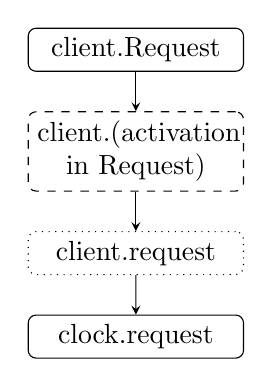
\begin{tikzpicture}[
    arrowstyle/.style={draw, -stealth},
    edge from parent/.style={draw, -stealth},
    reaction/.style={rectangle, draw, rounded corners=1mm, text width=2.5cm,
        text centered, anchor=north},
    activation/.style={rectangle, draw, rounded corners=1mm, dashed, text width=2.5cm,
        text centered, anchor=north},
    push/.style={rectangle, draw, rounded corners=1mm, dotted, text width=2.5cm,
        text centered, anchor=north},
    level 1/.style={sibling distance=7.0cm},
    level 2/.style={sibling distance=4.0cm},
    level 3/.style={sibling distance=3.0cm},
    level distance=0.5cm, growth parent anchor=south
]
\node (Action) [reaction] {client.Request}
  child {
    node (Activation01) [activation] {client.(activation in Request)}
    child {
      node (Push01) [push] {client.request}
      child {
        node (Reaction01) [reaction] {clock.request}
      }
    }
  }
;
\end{tikzpicture}
\endgroup
%%}%
\cprotect\caption{Transaction diagram for the \verb+client.Request+ action of the Clock System}
\label{request_transaction}
\end{figure}

\begin{figure}
\centering
%%\resizebox{\textwidth}{!}{%
\begingroup
\fontsize{10pt}{12pt}\selectfont
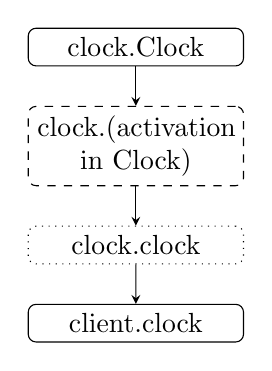
\begin{tikzpicture}[
    arrowstyle/.style={draw, -stealth},
    edge from parent/.style={draw, -stealth},
    reaction/.style={rectangle, draw, rounded corners=1mm, text width=2.5cm,
        text centered, anchor=north},
    activation/.style={rectangle, draw, rounded corners=1mm, dashed, text width=2.5cm,
        text centered, anchor=north},
    push/.style={rectangle, draw, rounded corners=1mm, dotted, text width=2.5cm,
        text centered, anchor=north},
    level 1/.style={sibling distance=7.0cm},
    level 2/.style={sibling distance=4.0cm},
    level 3/.style={sibling distance=3.0cm},
    level distance=0.5cm, growth parent anchor=south
]
\node (Action) [reaction] {clock.Clock}
  child {
    node (Activation01) [activation] {clock.(activation in Clock)}
    child {
      node (Push01) [push] {clock.clock}
      child {
        node (Reaction01) [reaction] {client.clock}
      }
    }
  }
;
\end{tikzpicture}
\endgroup
%%}%
\cprotect\caption{Transaction diagram for the \verb+clock.Clock+ action of the Clock System}
\label{clock_transaction}
\end{figure}

\section{Properties of Composition}
\label{propcomp}
In this section, we examine various features related to reactive components and composition.
Substitutional equivalence for reactive components is demonstrated by outlining a procedure for in-lining sub-components.
Hazards of composition, namely, non-deterministic state transitions resulting from conflicting and recursive composition, are identified and a means of detecting them is proposed.
The issue of decomposition is considered and \emph{pull ports} are introduced as a mechanism for decomposition.

\begin{figure}
\begin{verbatim}
component System {
  /* Substitution of clock component. */
  var int clock_counter (0)
  var bool clock_flag (false)
  push clock_clock(int t)

  reaction clock_request() clock_flag := true

  clock_Clock: clock_flag -> clock_flag := false activates clock_clock(clock_counter)

  clock_Tick: clock_counter := clock_counter + 1

  /* Substitution of client component. */
  var bool client_flag (false)
  push client_request()

  client_Request: !client_flag -> client_flag := true activates client_request()

  reaction client_clock(int t) client_flag := false || /* do something with t */

  bind {
    client_request -> clock_request
    clock_clock -> client_clock
  }
}
\end{verbatim}
\caption[Substitution of sub-components for the Clock System]{Substitution of state variables, ports, actions, and reactions for the sub-components of the System component of the Clock System}
\label{se1}
\end{figure}

\begin{figure}
\begin{verbatim}
component System {
  var int clock_counter (0)
  var bool clock_flag (false)
  var bool client_flag (false)
  push clock_clock(int t)
  push client_request()

  clock_Clock: clock_flag -> clock_flag, client_flag :=
    false, false activates clock_clock(clock_counter) ||
    /* do something with clock_counter */

  client_Request: !client_flag -> client_flag, clock_flag :=
    true, true activates client_request()

  clock_Tick: clock_counter := clock_counter + 1
}
\end{verbatim}
\caption[Simplification of expanded System component of the Clock System]{Simplifications of ports, bindings, and transitions in the expanded System component of the Clock System}
\label{se2}
\end{figure}

\subsection{Substitutional Equivalence}
\label{substitutional_equivalence}
For reactive components, substitutional equivalence means that a sub-component can be replaced with its definition and the result is a well-defined entity in the model.
To this end, a procedure for substituting the definition of a sub-component involves 1) renaming and adding all state variables, ports, actions, and reactions to the parent component and 2) simplifying bindings by substituting the transitions associated with a reaction into the action or reaction that activates the reaction in question.

To illustrate, Figure~\ref{se1} shows the result of substituting state variables, ports, actions, and reactions into the System component of Figure~\ref{system_component}.
Identifiers in the sub-components have been prefixed with the name of the sub-component instance to avoid name clashes.
For example, the \verb+request+ reaction in the \verb+clock+ sub-component has been renamed to \verb+clock_request+.
Figure~\ref{se2} shows the result of simplifying bindings and state transitions.
Note that the push ports have been retained for subsequent composition, i.e., the System component may be a component in a larger system.
The result is a reactive component whose ``size'' in terms of state variables, actions, and reactions is the sum of the sizes  of its constituent components.
Substituting the definition of the Clock component and Client components into the System component confirms the intuition that the flag variable in the client and flag variable in the clock are the same since 1) initially they have the same value and 2) they take on the same value in every state transition.

\subsection{Determinism and Composition}
\label{determinism}

\begin{figure}
\centering
%%\resizebox{\textwidth}{!}{%
\begingroup
\fontsize{10pt}{12pt}\selectfont
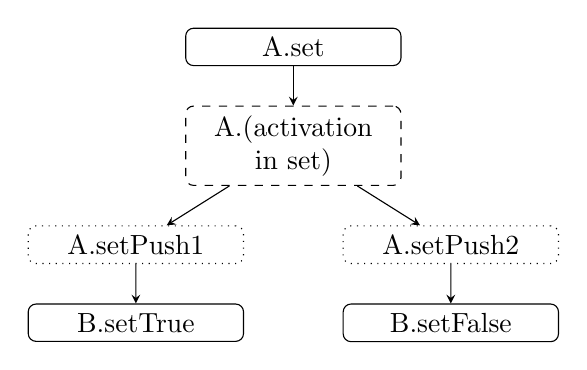
\begin{tikzpicture}[
    arrowstyle/.style={draw, -stealth},
    edge from parent/.style={draw, -stealth},
    reaction/.style={rectangle, draw, rounded corners=1mm, text width=2.5cm,
        text centered, anchor=north},
    activation/.style={rectangle, draw, rounded corners=1mm, dashed, text width=2.5cm,
        text centered, anchor=north},
    push/.style={rectangle, draw, rounded corners=1mm, dotted, text width=2.5cm,
        text centered, anchor=north},
    level 1/.style={sibling distance=7.0cm},
    level 2/.style={sibling distance=4.0cm},
    level 3/.style={sibling distance=3.0cm},
    level distance=0.5cm, growth parent anchor=south
]
\node (Action) [reaction] {A.set}
  child {
    node (Activation01) [activation] {A.(activation in set)}
    child {
      node (Push01) [push] {A.setPush1}
      child {
        node (Reaction01) [reaction] {B.setTrue}
      }
    }
    child {
      node (Push02) [push] {A.setPush2}
      child {
        node (Reaction02) [reaction] {B.setFalse}
      }
    }
  }
;
\end{tikzpicture}
\endgroup
%%}%
\caption{Transaction diagram for a non-deterministic transaction}
\label{ndt}
\end{figure}

The result of composing two well-defined reactive components may yield a system that is non-deterministic.
The two ``hazards'' that must be avoided are non-deterministic assignment to state variables and recursively activated reactions.
Non-deterministic assignment results when the next value for a state variable is not well defined due to the inclusion of two or more transitions in a transaction that operate on the state variable.
To illustrate, consider the transaction depicted in Figure~\ref{ndt}.
The set action of component A has a single activation that activates both the setPush1 and setPush2 push ports.
The setPush1 port is bound to the setTrue reaction of component B while the setPush2 port is bound to the setFalse reaction of the same component B.
Suppose that the setTrue reaction sets a flag to true while the setFalse reaction sets the same flag to false.
The transaction is non-deterministic because the value of the flag after the (A,set) transaction may either be true or false.
An offending pair of transitions may appear anywhere in a transaction graph given that arbitrary transaction graphs may be constructed through composition.
If the underlying language used to define transitions admits pointers, dynamic memory, if statements, and loops (i.e., is Turing-complete), then the problem of determining if two transitions operate on the same state variable is undecidable in general~\cite{Landi:1992:USA:161494.161501, Ramalingam:1994:UA:186025.186041}.
For a transaction graph $G$, instances $i_1$ and $i_2$, and actions/reactions $t_1$ and $t_2$, a necessary (but not sufficient) condition for non-deterministic assignment $\mathit{NDA}$ from composition is $\mathit{NDA}(G): \exists (i_1, t_1), (i_2, t_2) \in G.N, i_1 = i_2, t_1 \ne t_2$ which says that the transaction must contain two different transitions involving the same component instance.

A recursively activated transition occurs when the transaction graph has a cycle.
The execution of such a transaction may result in well-defined next values for all state variables assuming that 1)~the recursion is bounded and 2)~the parameters passed to every reaction result in identical computations.
A transaction may be analyzed like a traditional transformational program since it has finite input, a finite output, and should terminate.
The first problem, then, is a thinly disguised version of the halting problem since it asks if a computation (the transaction) expressed in a Turing-complete language terminates (has bounded recursion)~\cite{Turing01011937, davis1958computability}.
A bounded recursion means that the execution of the transaction will generate a bounded number of activations $A$.
For each activation $a \in A$, we must determine what state is updated by $a$.
If the language is Turing-complete, then this problem is undecidable in general~\cite{Landi:1992:USA:161494.161501, Ramalingam:1994:UA:186025.186041}.
For state variables that are updated by more than one activation, we must then show that each activation sets the state variable to the exact same next state.
If we treat each activation as a program, then we require a function that determines if two (arbitrary) programs compute the same function, which is again, undecidable in general~\cite{Rice:53}.

The difficulty of detecting composition that results in non-deterministic assignments suggests that these problems are best checked by a machine.
That is, an implementation of reactive components may prevent non-deterministic assignment by checking that $\mathit{NDA}(G)$ is false for all transaction graphs in the system.
Similarly, an implementation may check for recursive activation by checking for cycles in transaction graphs.
Both of these approaches are used by the implementation described in Section~\ref{sound_composition}.

\subsection{Decomposition, Getters, and Pull Ports}
\label{decomposition}
Substitutional equivalence implies that the process of substituting the definition of a sub-component into a parent component may be reversed and that sub-components may be ``factored out'' of an existing component, e.g., for reuse with other components.
%% One motivation for extracting sub-components is to support the software engineering practice of refactoring where common code is extracted so that it can be reused in various places.

Another motivation for decomposition is potentially increased performance through parallelism.
Recall that true concurrency in reactive components is modeled as the serial and non-deterministic execution of atomic actions.
Two transactions can be safely executed concurrently if it can be shown that the state variables involved in each transaction are disjoint.
As was previously mentioned, making this determination is undecidable for Turing-complete languages in the general case.
However, the problem becomes decidable if the component instance is used as a proxy for its constituent state variables.
Let $\mathit{rw}: t \to \{ \mathit{Read}, \mathit{Write} \}$ be a function that maps a transition to a value indicating that variables are read-only during the transition or written in some way.
Two instance/transition pairs are independent ($\mathit{indp}$) if either the instances are different or at most one of the transitions writes to the variables of the instance:
\begin{equation}
\mathit{indp}((i_1, t_1), (i_2, t_2)): i_1 \ne i_2 \lor \lnot (\mathit{rw}(t_1) = \mathit{Write} \land \mathit{rw}(t_2) = \mathit{Write})
\end{equation}
Two transaction graphs are independent if all of their nodes are independent $\mathit{indp}(G_1, G_2) = \forall (i_1, t_1) \in G_1.N, (i_2, t_2) \in G_2.N \; \mathit{indp}((i_1, t_1), (i_2, t_2))$.
The significance of the preceding analysis is that the determination about what actions can be executed concurrently becomes machine checkable due to the strong guarantee that state variables belonging to an instance can only be modified by the transitions of that instance.

To illustrate the mechanisms required for decomposition, we will factor out a Counter component from the Clock component of Figure~\ref{clock_component} and then rewrite the Clock component using the Counter component.
Upon inspection, the \verb+Tick+ action and \verb+request+ reaction can be executed concurrently since the state variables involved in each transition are disjoint.
Figure~\ref{counter_component} shows the Counter component which consists of a \verb+counter+ state variable.
The \verb+Tick+ action can be moved to the Counter component without complication.
The \verb+Clock+ action of the Clock component \emph{reads} the value of \verb+counter+ which suggests that a mechanism for accessing the state variables in a component is required.
Thus, we introduce the notion of a \emph{getter} method which can be called on a component to produce a value that may be derived from its state variables.
In the Counter component, the \verb+getCounter+ getter returns the current value of the counter.
A getter is not allowed to modify the state of a component and may only be invoked in the immutable phase.
These semantics preserve the strict separation of immutable phase and mutable phase.
When analyzing composition, a getter is treated like a transition that reads the state variable of the corresponding instance.
Figure~\ref{factored_clock_component} shows the Clock component rewritten to use a Counter sub-component and a getter.

\begin{figure}
\begin{verbatim}
component Counter {
  var int counter (0)

  Tick: counter := counter + 1

  getCounter() int {
    return counter
  }
}
\end{verbatim}
\caption{Definition of the Counter component of the Factored Clock System}
\label{counter_component}
\end{figure}

\begin{figure}
\begin{verbatim}
component Clock {
  var Counter c
  var bool flag (false)
  push clock(int t)

  reaction request() flag := true

  Clock: flag -> flag := false activates clock(c.getCounter())
}
\end{verbatim}
\caption{Definition of the Clock component of the Factored Clock System}
\label{factored_clock_component}
\end{figure}

The logic associated with the \verb+flag+ state variable represents a generic request-response protocol except for the call to \verb+c.getCounter()+.
To indirect the call to \verb+c.getCounter()+ we introduce the notion of a \emph{pull port}.
A pull port represents an external value dependency.
A component can demand a value from the pull port in the immutable phase.
Like push ports, pull ports have an active and passive side.
The active side represents the caller and the passive side represents the callee.
Getters are sufficient to realize the passive side of a pull port.
Every active pull port must be bound to exactly one passive pull port via composition.
Figure~\ref{request_response_component} shows a component that implements the request-response protocol using a pull port \verb+getValue+.
Figure~\ref{factored2_clock_component} shows the Clock component written in terms of the Counter and RequestResponse components.
An \verb+export+ directive allows reactions, getters, and ports in sub-components to be available in the interface of the encapsulating component.

\begin{figure}
\begin{verbatim}
component RequestResponse {
  var bool flag (false)
  pull getValue() int
  push response(int t)

  reaction request() flag := true

  Response: flag -> flag := false activates response(getValue())
}
\end{verbatim}
\caption{Definition of the RequestResponse component of the Factored Clock System}
\label{request_response_component}
\end{figure}

\begin{figure}
\begin{verbatim}
component Clock {
  var Counter c
  var RequestResponse rr
  push request()
  push clock(int t)

  bind {
    c.getCounter -> rr.getValue
  }

  export rr.request as request
  export rr.response as clock
}
\end{verbatim}
\caption{Definition of the Clock component of the Factored Clock System (fully-factored)}
\label{factored2_clock_component}
\end{figure}

Pull ports are subject to a hazard of composition similar to the recursive activation hazard of push ports.
A cycle in the graph of composed pull ports is equivalent to a recursively defined function.
The recursion may be bounded but this is undecidable in the general case.
Consequently, an implementation may reject recursively defined getters and pull ports.

\section{Summary}
In this chapter, we have presented the reactive component model for reactive programs.
A reactive component consists of a set of state variables and transitions that are private to the component.
The interface of a reactive component consists of push ports and reactions, which allow a component to trigger a transition in another component, and pull ports and getters, which allow a component to access the state of another component.
The external or visible behavior of a reactive component can be traced through its interface, specifically its push ports.
The internal details of a component can often be abstracted away to permit reasoning about the behavior of a composed system at various levels of detail.
Composition is achieved through recursive encapsulation (sub-components) and explicit port binding and satisfies the requirements for principled composition set forth in Section~\ref{challenges}.
As demonstrated in Section~\ref{substitutional_equivalence}, the definitions of sub-components can be substituted into the containing component resulting in an equivalent system (substitutional equivalence).
Similarly, sub-components may be ``factored out'' by using pull ports and getters to safely access the state of the sub-components.

The private nature of state variables and transitions causes properties established from the text of a component to be preserved through composition.
Composition links transitions to form an atomic transaction that allows the properties of one component to be related to another component.
When the sub-components of a component are protected from further composition, the properties derived from their interactions are preserved as the parent component is composed.
Property-preserving composition is essential for reasoning about systems in a hierarchical and/or modular fashion.

The result of composing reactive components is either well-defined due to the atomic nature of transactions or illegal due to the composition hazards of recursive transactions and non-deterministic state transitions.
Analysis of these hazards at the state variable level is impossible due to the undecidable nature of their sub-problems.
This suggests that implementations may restrict composition to prevent the conditions necessary for recursive transactions and non-deterministic state transitions.
The main concession is allowing a component instance to proxy for its state variables.
The problem of detecting recursive transactions, then, can be posed as the problem of detecting cycles in a directed graph.
Similarly, the problem of detecting potentially non-deterministic state transitions is reduced to a set membership problem.
Valid systems that fail the check for non-deterministic state transitions using component instance proxies can be refactored by decomposing  the offending components.

\chapter{Reactive Component Language\label{language}}

\begin{quote}
In theory, there is no difference between theory and practice. \linebreak
But, in practice, there is.  \emph{Anonymous}
\end{quote}

In this chapter, we present a programming language for reactive components.
We state the motivation for the language, our assumptions for tractability, and the features that guided our design.
We then show how reactive components are expressed in the language and we conclude with illustrative examples.

\section{Introduction}

An implementation of the reactive component model presented in chapter~\ref{model} is necessary for at least three reasons.
First and foremost, an implementation tests the practicality of the model.
The act of implementing the model can help to evaluate whether the assumptions upon which the model is founded can be realized using existing techniques.
Conversely, an implementation can suggest restrictions to the model that are necessary to produce an effective implementation.
An example of this was seen in section~\ref{propcomp} where the component instance was used as proxy for its state variables for the purpose of determining which variables were involved in a transaction.
Implementation forces one to supply and consider details that can either qualify or disqualify a model as a practical engineering tool.
This is consistent with the emerging attitude in systems research that all new ideas and techniques must be accompanied by relevant tools and evaluations to show their feasibility.

Second, language support for a model is beneficial because it closes the semantic gap between reasoning and implementation.
The importance of language support can be seen in techniques like structured programming~\cite{dahl1972structured} and object-oriented programming~\cite{booch1982object}.
While these techniques can be applied in virtually any setting, their lasting utility is derived from their implementation in a variety of programming languages.
Providing language support for a model raises the level of abstraction and allows reasoning about a system directly from its specification instead of reasoning in one set of semantics while implementing in another which can be tedious and error-prone.
Language support allows developers to rely on the consistent application of the semantics of the model through strict enforcement, e.g., checking by a compiler.

Third, an implementation is necessary to demonstrate that the model can be applied successfully to real-world design and implementation problems.
That is, given a platform for reactive components, we can design, construct, and evaluate systems based on the reactive component paradigm.
Furthermore, we can evaluate critically the design and implementation processes that the model and platform encourage.
By comparing implementations of similar systems in two different models, we can gain insight into the strengths and weaknesses of the model.
These ideas will be explored further in chapter~\ref{evaluation}.

\section{Technical Agenda}

Through the process of designing and implementing a language for reactive components, we seek to answer the following questions.

\paragraph{What techniques, assumptions, and approximations are necessary to organize and enforce the semantics of reactive components?}
An implementation of reactive components should provide three things.
First, an implementation should provide a mechanism for declaring and defining the various elements of the reactive component model.
One way of doing this is to define a language with syntax for actions, reactions, getters, activations, etc.
Another way is to programmatically assemble the reactive components using a library in another language.
As previously discussed, this approach forces one to reason about a system using one set of semantics while implementing it under a different set of semantics which can be tedious and error prone.

Second, an implementation should provide the checks necessary to enforce the semantics of reactive components.
The checks of interest are 1) the separation of the immutable and mutable phase, 2) the binding state of pull ports, 3) the binding state of reactions, and 4) the detection of non-deterministic state transitions arising from composition.
These checks may be carried out by a compiler/interpreter or developers or not performed at all.
Not performing the checks is unacceptable due to the subtlety associated with developing correct reactive programs.
In this scenario, the semantics of reactive components would be enforced through convention which is easily violated.
Similarly, placing the burden on developers is unacceptable due to the amount of detail that must be considered.
Thus, the implementation must enforce the semantics of reactive components through adequate checking.

To enforce the semantics of reactive components, the compiler or interpreter must have sufficient semantic knowledge to distinguish correct programs from potentially incorrect programs.
To illustrate, consider the problem of ensuring that the state of a component does not change during the immutable phase of a transition.
We observe that that an action/reaction is similar to a method.
Based on this observation, checking the immutability of a component in the immutable phase should be similar to checking for \verb+const+ correctness in C++.
In C++, the \verb+const+ correctness check is performed early in the compilation process when the program is represented as an abstract syntax tree (AST) with full semantic information, as opposed to late in the process where the program is represented by machine instructions with very limited semantic information.
From this, we observe that checking is made possible or easier by 1) adding features to the language which provide the necessary semantic information and 2) performing the checks early in the translation process.
An existing language or code might not provide enough detail to facilitate the necessary checks while a lack of detail may prevent efficient checking.
Along the same lines, an implementation may have to make conservative assumptions to enforce the semantics of reactive components.
As was seen in section~\ref{propcomp}, allowing a component instance to serve as a proxy for all of its state variables allows the check for non-deterministic state transitions to be implemented using known techniques.

The final basic feature that should be supplied is a scheduler that executes the system described by the user's program.
The scheduler will be discussed in chapter~\ref{implementation}.

\paragraph{What techniques, assumptions, and approximations are necessary to allow the use of reference semantics and linked data structures in the state and transitions of reactive components?}
Formal models for reactive systems typically use mathematically friendly data-types to make proofs easier.
However, reference semantics and the linked data structures they make possible are a critical part of modern software engineering.
As two of our objectives are practicality and utility, a language for reactive components must support reference semantics and linked data structures.
The potential hazard created by reference semantics is that the state of one component becomes accessible in another component.
This means that the state of a component may not be solely under the control of the transitions for that component.
Consequently, the properties associated with that component carry no weight as they could be violated by the other components manipulating that state.
Furthermore, an implementation that chooses to concurrently execute seemingly independent transactions may cause data corruption as two transactions may manipulate the same state in an uncoordinated fashion.
Thus, an implementation of reactive components must take special care to preserve the isolation of state among reactive components when supporting references and linked data structures.

\paragraph{What techniques, assumptions, and approximations are necessary to facilitate efficient communication between reactive components?}
Linked data structures create the opportunity for efficient communication between components.
There are three modes by which a component (sender) can share information with another component (receiver) as they interact through push ports and pull ports.
First, the sender may use \emph{value semantics} where it provides a complete copy of the value to be communicated.
This approach is reasonable for values like numbers and small records.
Second, a sender may use \emph{reference semantics} where it provides a pointer (reference) to the data to be communicated.
The approach is reasonable when the sender offers up a large data structure.
The receiver is responsible for copying any data that needs to be retained.
When using reference semantics, receivers may read the data structure represented by the pointer but may not alter or remember the original data structure in any way.
Third, a sender may use \emph{move semantics} where it provides a pointer to a data structure that the receiver may adopt as its own.
In this case, the sender promises to ``forget'' the data structure as the receiver is the new owner of the data structure.
Move semantics are appropriate when the size of the data to be communicated is large, there is a single receiver, and the sender does not need to retain the data.
These conditions arise is situations like network stacks and pipelines.
Without move semantics, the practicality of the reactive component model is greatly diminished.

%% \paragraph{Direct implementation and strict enforcement.}
%% The language should facilitate the construction of reactive systems through the direct definition and composition of reactive components.
%% The obvious alternative is to encode reactive components in another language or set of languages.
%% As previously mentioned, we feel that this alternative is unacceptable as it forces one to implement a system in one language and set of semantics while reasoning about the system in another set of semantics.
%% Defining a new language admits opportunities to introduce language features that allow the semantics of the model to be strictly enforced.
%% An existing language may lack these features which means that the model would be enforced through convention and programmer effort.
%% We view this alternative to be unacceptable given the subtlety associated with developing correct reactive programs.
%% As a matter of personal preference, we will attempt to check reactive component semantics at ``compile-time.''
%% So what?  What important question does this answer?

%% \section{Approach}
%% Our approach to implementing reactive components is to define a high-level programming language for reactive components and implement that language in an interpreter.
%% The two alternatives to a high-level programming language are a low-level byte-code and a coordination language.
%% The main purpose of byte-code is to describe a transformation computation for a real or virtual machine.
%% Many of the interesting elements of reactive components, like actions, reactions, getters, push ports, pull ports, activations, and bindings are more declarative in nature.
%% Thus, the initial effort should be to capture these elements using a high-level language.
%% The choice to implement an interpreter made the task more tractable as it avoids code generation, linking, and loading.
%% However, in moving from the interpreter to a compiler, the processes of code generation, linking, and loading must provide the same guarantees that are enforced by the high-level language.
%% We describe the challenges of moving from interpreter to compiler in chapter~\ref{future_work}.

%% We elected to not implement reactive components as a coordination language due to the interplay between reactive and transformational semantics.
%% The coordination language approach involves two completely separate languages.
%% The reactive language would encode systems using the elements of the reactive component model, e.g., components, actions, push ports, etc. while the transformation language would define all of the types and computation performed on those types.
%% For this approach to be viable, the transformational language must guarantee that no component changes state during the immutable phase of a transition and that the state of each component remain isolated.
%% An ordinary programmer with a sufficiently powerful transformational language, like C, C++, or Java, can easily violate these requirements.
%% Based on this observation, we elected to define a language for reactive components that includes a \emph{transformational basis} that has been modified to provide the guarantees necessary for reactive component semantics.

\section{Preliminaries}

\paragraph{Design sketch.}
We adopt the Go~\cite{go} programming language as the foundation for a programming language based on reactive components.
Actions, reactions, getters, initializers, and bindings are expressed using Go's syntax for methods.
Component types are constructed using the syntax of structs.
Push ports and pull ports are fields of a component.
To enforce the immutable phase and facilitate checks for reference semantics, we introduced syntax that prevents the abuse of pointers.
Activations in the model correspond to an activation statement that activates push ports and contains the mutable phase of a state transition.
Move semantics are realized through a new \emph{heap} type and associated operations.

Go is an imperative programming language with a straightforward type system and expressions and statements resembling C.
Go supports methods but places no emphasis on an inheritance hierarchy.
In the same vein, Go does not have constructors, destructors, function overloading, and operator overloading.
This combination, in our opinion, makes Go an attractive foundation for a language for reactive components since it is tractable in implementation and approachable by a general audience.
We defer to Go's syntax and semantics for types, declarations, statements, and expressions.
We will not discuss the syntax and semantics of Go except when they interact with the semantics of reactive components.
Our implementation of Go is intentionally incomplete as a full implementation is beyond the scope of this project.

\paragraph{Static system assumption.}
To make implementation more tractable, we will assume that the systems to be implemented have a static topology meaning that all reactive components are statically allocated.
Both finite state and infinite state (subject to system resource limits) reactive components are permitted, but both the number and configurations of reactive components in a system are fixed.
This is equivalent to systems that assume a fixed number of actors and is roughly equivalent to systems that assume a fixed number of threads.
These assumptions are common in embedded and real-time systems due to the combination of limited resources and a need for predictability.
We also believe these assumptions are common in less constrained environments as the number of threads is often fixed by the design, e.g., only a fixed number of concurrent activities is needed, or the number of threads is limited by the number of available physical cores.
Thus, even with the static system assumption, an implementation of the model is still applicable to many systems of interest.
We leave the implementation of extensions that facilitate the dynamic creation and binding of reactive components for future work.

\paragraph{Memory model.}
A memory address may refer to a location in the constant segment, a stack, the static component segment, or a heap.
The constant segment is used to store aggregate literals like string constants.
Function parameters and local variables are allocated on a call stack as they are in C or C++.
The static component segment contains statically allocated components.

Let $f(c)$ be a function that returns the set of addresses $[c,c+sizeof(T))$ if $c$ is a pointer and $\emptyset$ otherwise.
Let $c$ be a pointer to a component of type $T$.
Assuming statically allocated components, the set of addresses $S = f(c)$ refers to a block of addresses with the same size as $T$ in the static component segment.
That is $S$ contains the addresses for the \emph{statically} allocated state of the component indicated by $c$.
Let $F(A) = \cup_{a \in A} f(a)$.
Let $C$ be the transitive closure of $F$ applied to $S$.
$C$ contains the set of memory addresses that contain the state of component $c$.
The set $H = C \setminus S$ contains the \emph{dynamically} allocated state of the component indicated by $c$.
Dynamically allocated state is contained in a heap.
Let $c_x$ and $c_y$ be two different components and their corresponding state $C_x$ and $C_y$.
The semantics of reactive components require that the state of each component be disjoint or $C_x \cap C_y = \emptyset$.
The static component segment and the heaps contain all of the mutable state in the system.
Mutable state outside of a component, e.g., a global variable, is prohibited as it may introduce a data race.

Part of our approach to maintaining disjoint state is preventing the formation of arbitrary pointers that would allow one component to access the state of another component.
Consequently, pointer arithmetic and casts from numeric values are not allowed.
Manually deallocating memory may result in dangling pointers~\cite{dangle} that may point to state in another component.
Consequently, some form of automatic memory management is necessary with the two primary candidates being reference counting and garbage collection.
Our implementation uses garbage collection and is described in chapter~\ref{implementation}.
%% Logically, then, each component has its own heap from which it can allocate memory.

%% A feature in the language is loosely classified as either \emph{reactive}, \emph{transformational}, or \emph{provisional}.
%% The features of the reactive component model, e.g., actions, reactions, etc., have corresponding features in the language.
%% The features used for describing state and state transformations, e.g., types, expressions, statements, functions, methods, etc., are generally useful in transformational programs.
%% Provisional features are elements that are not in the reactive component model but are necessary to enforce the semantics of the model or a desired feature.
%% This chapter focuses on the syntax and semantics of a programming language based on reactive components while chapter~\ref{implementation} focuses on the techniques used to implement the features.

\section{Programming Language}

\paragraph{Components.}
A component resembles a \verb+struct+ in Go since it is a group of named state variables.
A component, then, is defined with the following syntax:
\begin{verbatim}
type identifier component { field list };
\end{verbatim}
For example,
\begin{verbatim}
type Clock component {
  flag bool;
  counter uint;
};
\end{verbatim}
introduces a type named \verb+Clock+ that is a reactive component with two fields (state variables).
The type of a field may be another component type to support recursive encapsulation.

\paragraph{Receivers.}
A method in Go has one of the following two forms:
\begin{verbatim}
func (identifier typeName) methodName signature body
func (identifier *typeName) methodName signature body
\end{verbatim}
The first form operates on a copy of a value of type \verb+typeName+.
The second form operates on a pointer to a value of type \verb+typeName+.
The parameter \verb+identifier+ performs the same function as the \verb+this+ keyword in C++ and Java.
The syntax \verb+(identifier typeName)+ is called a receiver and the syntax \verb+(identifier *typeName)+ is called a pointer receiver.
Many of the syntactic elements introduced for reactive components use a pointer receiver.

\paragraph{Intrinsic and dereference mutability.}
Variables and parameters may be declared with an \emph{intrinsic mutability} and a \emph{dereference mutability}.
Intrinsic mutability limits the operations that can be performed on an lvalue of the variable or parameter while dereference mutability limits the operations that can be performed on lvalues derived from the rvalue of the variable or parameter.
By default, variables and parameters have mutable intrinsic and dereference mutability.
The following code is legal and sets \verb+z+ to 6.
\begin{verbatim}
var x uint = 3;
var y *uint = &x;
var z = x + *y;
\end{verbatim}

Declaring a variable or parameter to have immutable intrinsic mutability (\verb+const+) prevents the variable or parameter from being changed after it is initialized.
The following code is illegal:
\begin{verbatim}
var x const uint = 3;
x = 4; // Illegal
\end{verbatim}
Immutable intrinsic mutability is enforced when taking the address of a variable or parameter:
\begin{verbatim}
var x const uint = 3;
var y *uint = &x;        // Illegal
var z $const *uint = &x; // Legal
var a uint = *z;         // Legal
*z = 5;                  // Illegal
\end{verbatim}
The second line is illegal because \verb+x+ could change through a statement like \verb+*y = 5;+.
The third line causes \verb+z+ to have immutable dereference mutability (\verb|$const|).
The expression \verb+*z+ can serve as an rvalue (line 4) but it cannot serve as an lvalue (line 5).

Dereference mutability is ``sticky.''
For example:
\begin{verbatim}
var x $const **uint = ...;
var y $const *uint = *x; // Legal
var z *uint = *x;        // Illegal
\end{verbatim}
The second line honors the guarantee that all of the memory accessible through \verb+x+ is immutable.
Dereference mutability is checked in assignment and calls.
Dereference mutability affects type from which lvalues can be derived, namely, pointers and slices (indexable pointers).
Immutable dereference mutability is one of the techniques that is used to enforce the immutable phase of state transitions.

The second kind of mutability is called \emph{foreign} mutability.
Foreign mutability is like immutable mutability with the added condition that an address with foreign mutability cannot be stored in a heap.
The primary application of foreign mutability is to support reference semantics for communication while enforcing the isolation of heaps.
\begin{verbatim}
var x $foreign *uint = ...;
var y **uint = new (*uint);
*x = 3;                            // Illegal
*y = x;                            // Illegal
var z $foreign *uint = x;          // Legal
\end{verbatim}
The third line is illegal because the lvalue given by \verb+*x+ is immutable.
The fourth line is illegal because it casts away the \verb|$foreign| of \verb+x+.
(Notice that declaring \verb+y+ with \verb|$foreign| would cause the lvalue to be immutable.)
The fifth line is legal because the lvalue is mutable and the \verb|$foreign| is preserved.
The consequence of these semantics is that variables that contain pointers that are declared \verb|$foreign| may only be stored on the stack.

%% Table~\ref{mutability} describes how the intrinsic and dereference mutability is computed for various expressions.
%% The operation of interest is the dereference operation which shows how dereference mutability is ``sticky'' and conservatively assumes that all pointers refer to an address on the heap.

The following checks are applied to assignment statements:
\begin{enumerate}
\item The lvalue and rvalue must be type compatible.
\item The lvalue must have mutable intrinsic mutability.
\item If the type involved contains a pointer or slice, check for compatible dereference mutability in table~\ref{assignmut}.
  Essentially, the dereference mutability of the lvalue must be at least as ``weak'' as the dereference mutability of the rvalue.
  This enforces the ``stickiness'' of dereference mutability.
\end{enumerate}

%% \begin{table}
%%   \centering
%%   \begin{tabular}{ccccp{1.75cm}cccc}
%%     Kind & Seg & Intrin & Deref & Op & Kind & Seg & Intrin & Deref \\
%%     \hline
%%     lvalue & S & A & B & load              & rvalue & S    & A & B \\
%%     rvalue & S & A & B & deref (\verb+*+)  & lvalue & heap & B & B \\
%%     lvalue & S & A & B & ref (\verb+&+)    & rvalue & S    & A & B \\
%%     lvalue & S & A & B & select (\verb+.+) & lvalue & S    & A & B \\
%%     lvalue & S & A & B & index (\verb+[]+) & lvalue & S    & A & B \\
%%   \end{tabular}
%%   \caption{Intrinsic and dereference mutability for various operations\label{mutability}.  The possible choices for segment are constant, stack or heap (includes the component segment).  The possible choices for the intrinsic and dereference mutability are mutable, immutable, and foreign.}
%% \end{table}

\begin{table}
  \centering
  \begin{tabular}{cccc}
              & Mutable & Immutable & Foreign \\
    Mutable   & Yes     & No        & No      \\
    Immutable & Yes     & Yes       & No      \\
    Foreign   & Yes     & Yes       & Yes     \\
    \end{tabular}
  \caption{Dereference mutability compatibility for assignment.\label{assignmut}.  The rows represent the dereference mutability of the lvalue and the columns represent the dereference mutability of the rvalue.}
\end{table}

A parameter is \emph{foreign safe} if (1) the type of the parameter does not contain pointers or slices or (2) the parameter is declared with foreign dereference immutability.
A parameter list is foreign safe if all parameters in the list are foreign safe.
A signature (a parameter list with a return parameter) is foreign safe if the parameter list and return parameter are both foreign safe.

\paragraph{Initializers.}
A initializer is used to initialize the fields of a reactive component.
This allows one to initialize components before the scheduler starts.
This is necessary for establishing invariants as is commonly done in formal models, e.g., the \verb+initially+ section of UNITY~\cite{chandy1989parallel}.
An initializer has the form:
\begin{verbatim}
init (id *typeName) initializerName signature body
\end{verbatim}
An initializer is similar to a method but has additional semantics:
\begin{itemize}
\item An initializer must have a pointer receiver to a component type.
\item The signature must be foreign safe.
\item An initializer may only be invoked by another initializer.
\item An initializer sets the heap on entry and resets the heap on exit so that all allocated memory is attributed to the receiver.
\end{itemize}

\paragraph{Instances.}
An instance is a top-level component.
An instance is declared with the following syntax:
\begin{verbatim}
instance identifier typeIdentifier initializerIdentifier (expressionList);
\end{verbatim}
For example, \verb+instance c Clock Init ();+ declares as instance named \verb+c+ of type \verb+Clock+ and will call the initializer \verb+Init+ with an empty list of arguments.
The instance identifier must be unique, the type identifier must refer to a component, and the initializer must be declared for the component type.

\paragraph{Actions.}
An action has the form:
\begin{verbatim}
action (id $const *typeName) identifier (booleanExpression) body
\end{verbatim}
The immutable dereference mutability of the receiver enforces the immutable phase of transactions.
Actions may only be defined for component types.
The Boolean expression is the precondition of the action.
The receiver variable is in scope for the evaluation of the precondition.
The body contains the state transitions associated with the action.

\paragraph{Reactions.}
A reaction has the form:
\begin{verbatim}
reaction (id $const *typeName) identifier (parameterList) body
\end{verbatim}
As with actions, the immutable dereference mutability of the receiver enforces the immutable phase of transactions.
Reaction may only be defined for component types.
The name of a reaction is used when binding.
The parameter list declares the parameters that are passed to the reaction.
The parameter list must be foreign safe.
This prevents the reaction from storing memory addresses from the component that activated the reaction.
The body contains the state transitions associated with the reaction.

\paragraph{Push ports.}
A push port is declared as a field of a component with push port type.
A push port type has the form:
\begin{verbatim}
push (parameterList)
\end{verbatim}
The parameter list declares the parameters that are passed to any bound reaction.
The parameter list must be foreign safe.
The following example declares a push port named \verb+response+ in the \verb+Clock+ component:
\begin{verbatim}
type Clock component {
  ...
  response push (t uint);
};
\end{verbatim}

\paragraph{Getters.}
A getter has the form:
\begin{verbatim}
getter (id $const *typeName) identifier signature body
\end{verbatim}
A getter is similar to a method but has additional semantics:
\begin{itemize}
\item A getter must have a pointer receiver to a component type declared with immutable dereference mutability.
\item The signature must be foreign safe.
\item A getter may only be invoked by another getter or an action or reaction in the immutable phase.
\item An getter sets the heap on entry and resets the heap on exit so that all allocated memory is attributed to the receiver.
\end{itemize}

\paragraph{Pull ports.}
A pull port is declared as a field of a component with pull port type.
A pull port type has the form:
\begin{verbatim}
pull (parameterList) returnParameter
\end{verbatim}
The parameter list declares the parameters that are passed to the bound getter.
The parameter list and return parameter must be foreign safe.
Pull ports are called like getters and place the same restriction on the caller, that is, a pull port may only be invoked by a getter or an action or reaction in the immutable phase.
The following example declares a pull port named \verb+isBufferFull+ in the \verb+Producer+ component:
\begin{verbatim}
type Producer component {
  ...
  isOutputBufferFull pull () bool;
};
\end{verbatim}
In this example, the intent of the pull port is to allow a \verb+Producer+ to interrogate the status of a down stream buffer to implement flow control.

\paragraph{Binders.}
Binders allow reactions to be associated with push ports and getters to be associated with pull ports.
Binding and recursive encapsulation are the two mechanisms for composing reactive components.
A binder has the form:
\begin{verbatim}
bind (id *typeName) identifier {
  bindStatement
  ...
}
\end{verbatim}
For example:
\begin{verbatim}
bind (this *System) TheBinder {
  this.producer.Out -> this.consumer.In;
  this.producer.isOutputBufferFull <- this.consumer.isInputBufferFull;
}
\end{verbatim}
The first statement of the example binds the \verb+Out+ push port of the \verb+System+'s \verb+producer+ to the \verb+In+ reaction of the \verb+System+'s \verb+consumer+\footnote{The select operator(\texttt{.}) automatically dereferences pointers.}.
The second statement of the example binds the \verb+isOutputBufferFull+ pull port of the \verb+System+'s \verb+producer+ to the \verb+isInputBufferFull+ getter of the \verb+System+'s \verb+consumer+.
The left side of a bind statement always refers to a port while the right side refers to a getter or action.
The direction of the arrow indicates the logical flow of information.
Thus, information flows from the push port to a reaction (\verb+->+) and information flows from the getter to a pull port (\verb+<-+).
A pull port must be bound to exactly one getter.
A reaction may be bound to at most one push port.
Binders are associated with a component type and evaluated for each instance of that component type.

\paragraph{Activations.}
Activations are the mechanism by which transactions extend to other components via push port/reaction bindings.
Activations also serve as the boundary between the immutable and mutable phases of a transaction.
An activation statement has the form:
\begin{verbatim}
activate portName (arguments) ... {
  statements
};
\end{verbatim}
Activation statements can only occur in the body of an action or a reaction.
Assume that the receiver of the action or reaction is named \verb+this+.
The expression \verb+this.portName+ must refer to a push port and the arguments passed to the push port must agree with its signature.
The list of push ports in an activate statement is optional.
When an activation statement is executed, the named push ports are activated meaning that the reactions bound to those push ports are activated with the given arguments.
This chaining of activations forms a transaction that resembles a tree where the root of the tree is a component/action pair, the other nodes are component/reaction pairs, and the links represent port activations.
Once all of the actions and reactions in the transaction have activated their last push port, they proceed to execute the body of the activate statements.
Recall that \verb+this+ has immutable dereference mutability.
Thus, all computation up to and including the last port activation constitutes the immutable phase of the transaction since the state of the components is not allowed to change.
Within the scope of the body, \verb+this+ changes to mutable dereference mutability which allows the state of a component to be changed.
Thus, the bodies of activation statements form the mutable phase of the transaction.
Actions and reactions return, i.e., the flow of control is halted, after the execution of the body of a activation statement.
Activate statements guarded by \verb+if+ statements facilitate \emph{conditional activation}.
An activate statement may not appear in another activate statement.

\paragraph{Arrays.}
A homogeneous group of sub-components may be declared using array syntax.
For example,
\begin{verbatim}
type System component {
  clock [5]Clock;
  ...
};
\end{verbatim}
declares 5 \verb+Clock+ sub-components.
To request the time from each \verb+Clock+, the \verb+System+ declares as array of 5 push ports and a \emph{dimensioned} action:
\begin{verbatim}
type System component {
  clock [5]Clock;
  push [5]request ();
  ...
};

[5] action (this $const *System) (...) {
  ...
  activate clock[IOTA] {
    ...
  };
}
\end{verbatim}
A dimensioned action is parameterized with an integral constant in the range $[0,dimension)$.
This constant is accessed through the \verb+IOTA+ symbol.
A push port in an array is activated by supplying an index.
The index expression must be constant to facilitate the check for sound composition.
Reactions may be dimensioned as well:
\begin{verbatim}
[5] reaction (this $const *System) clock (t int) { ... }
\end{verbatim}
A \verb+for+-loop over an integral range may be used to generate bindings without explicitly listing each binding.
For example:
\begin{verbatim}
bind (this *System) {
  for i ... 5 {
    this.request[i] -> this.clock[i].request;
  };
}
\end{verbatim}

\paragraph{Transferrable heaps.}
A key requirement for implementing reactive components is that the state of each component remain disjoint.
Foreign dereference mutability allows components to safely communicate with pointers because it ensures that those pointers are forgotten after the transaction.
For efficient communication, we also desire the ability to transfer a data structure (the heap) from one component (the sender) to another component (the receiver).
The sender offers the heap to its receivers and one of the receivers may claim the heap.
If the heap is accepted, the sender must forget all references to the heap.

A heap is a type so named because it resembles a heap used for dynamic memory allocation.
A heap has a distinguished root that contains the data structure that will be transferred.
A heap is entirely self-contained, that is, any pointer found in the heap may only point to an address in the heap.
This ensures that the receiver may not access state in the sender after a transfer.
Heaps may form hierarchies.

A heap is created with the \verb+new+ operator.
For example:
\begin{verbatim}
var x *heap int = new (heap int);
\end{verbatim}
creates new heap with an integer root.

A \verb+change+ statement allows one to access the root of the heap.
For example:
\begin{verbatim}
change (x, y) {
  *y = 3;
};
\end{verbatim}
In the example, \verb+x+ is a pointer to a heap and \verb+y+ is a variable that points to the root of the heap.
The root variable is valid for the scope introduced by the \verb+change+ statement.
The root variable will be set to \verb+nil+ if the heap is no longer valid.
Within the scope of the \verb+change+ statement, all other variables and parameters are re-entered with foreign dereference immutability.
This enforces the isolation of heaps by preventing the heap from storing a pointer that refers to a location in another heap.

Heaps are treated like a stack.
On entering an action or reaction, the stack of heaps contains a single heap:  the heap associated with the receiver component.
A \verb+change+ statement pushes a new heap on the stack.
All memory allocations are performed using the current heap.

A \verb+move+ expression allows a receiver to take ownership of a heap being offered by a sender.
For example:
\begin{verbatim}
var z *heap int = move (x);
\end{verbatim}
If \verb+x+ refers to a heap that has already been moved, i.e., claimed by this component or another component, then the result of the \verb+move+ is a \verb+nil+ pointer.
A \verb+change+ statement can be used to access the data in the heap after a successful \verb+move+.

A \verb+merge+ expression allows one to merge a heap into the current heap.
For example:
\begin{verbatim}
var x *uint = merge (z);
\end{verbatim}
A \verb+merge+ expression performs an implicit \verb+move+, that is, the heap given to \verb+merge+ need not be owned by the current component.
Similarly, a \verb+merge+ will return \verb+nil+ if the heap has already been claimed.

Operations on heaps, specifically, \verb+change+, \verb+move+, and \verb+merge+ are atomic within a transaction.
The reactive component model requires a clear distinction between the mutable phase and immutable phase and some causality in the immutable phase.
However, an implementation is free to execute immutable phases concurrently and/or mutable phases concurrently.
Consequently, different components may be performing heap operations on the same heap at the same time.
Thus, \verb+change+, \verb+move+, and \verb+merge+ are atomic with respect to each other.
These operations return \verb+nil+ indicating a failure.
For example, if two components attempt to \verb+move+ the same heap, one will succeed and the other will fail.

\section{TODO: Examples}

\section{TODO: Summary}

Revisit technical agenda and provide answers to the questions that were asked.

%% \section{BEGINNING OF UNADOPTED MATERIAL FROM PROPOSAL}

%% \paragraph{Compilation.}
%% To facilitate a design and development process based on composition and decomposition, we require a high-level language that resembles the model and examples presented in section~\ref{model}.
%% The goal of the compiler, then, is to translate the high-level language to the language of the $\alpha$-machine.
%% %% Complication typically consists of five phases corresponding to scanning, parsing, semantic analysis, optimization, and code generation.
%% In addition to conventional semantic analysis, e.g., type checking, the compiler will check that the reactive system is well-defined and provide a concurrency analysis to be used during scheduling.
%% %% Optimization is beyond the scope of this research.

%% Substitutional equivalence provides the logical foundation for testing well-definedness.
%% A system is represented as a top-level reactive component.
%% The input and output ports original to the top-level component can be converted to internal ports since the top-level component does not need an external interface.
%% Substitutional equivalence allows the declarations of member components to be replaced with their definitions according to the procedure outlined in section~\ref{model}.
%% This process can be repeated until all member components are ``inlined'' resulting in a top-level component that only contains state variables, internal ports, $\alpha$-statements, $\beta$-statements, and $\gamma$-statements.
%% At this point, all internal ports, $\gamma$-statements, and $\beta$-statements can be eliminated by substituting definitions.
%% The resulting top-level component only contains state variables and $\alpha$-statements.
%% To be a faithful implementation of the model, each $\alpha$-statement must be a deterministic state transformation.
%% The main challenge, then, lies in the co-design of a transformational language and checks for deterministic assignment.

%% At a high level, we desire to treat the transformation specified by an $\alpha$-statement as a function that maps a value representing the current state to a value representing the next state because it leads to a simple decidable check.
%% An $\alpha$-statement then consists of five parts:  a precondition list, a precondition function, an assignment list, an argument list, and an effect function.
%% The precondition list and argument list are lists of readable objects that form the arguments of the precondition function and effect function, respectively.
%% The assignment list is a list of writable objects that are assigned the values produced by the effect function (state variables that are not named in the assignment list retain their previous values and ports that are not named in the assignment list are undefined).
%% There is no notion of state or assignment inside the effect function, which thus resembles a pure functional or applicative program.
%% A conservative but decidable check, then, is to ensure that a writable object appears at most once in the assignment list.

%% %%Another concept implicit in the semantics of functional languages and their data structures is freedom from aliasing.
%% The approach outlined above hinges on the semantics of writable objects.
%% We define a writable object to be the name for an implied set of storage locations.
%% All elements in the set of storage locations for a scalar variable are updated in an assignment to the variable.
%% In contrast, only a subset of the set of storage locations for aggregate variables such as arrays and records may be updated in an assignment.
%% Variables can also name linked data structures where the set of locations is the transitive closure of a points-to analysis~\cite{hind2001pointer}.

%% For well-definedness, we require that the implied sets of storage locations for all writable objects be disjoint.
%% Thus, an assignment to two different variables in an $\alpha$-statement cannot update the same memory location.
%% The challenge then is to show that this condition holds initially and that it holds after the execution of each $\alpha$-statement.
%% This is the subject of pointer analysis~\cite{hind2001pointer} which is undecidable in general.
%% Components that communicate by passing data by reference as opposed to by value obviously violate this condition since multiple components may then reference the same memory locations.
%% Thus, data passed by reference through ports must have semantics that prevent concurrent updates, e.g., constant (read-only), copy-on-write, etc.
%% The goal then is to place appropriate restrictions on the language so as to make pointer analysis feasible and enable the safe sharing of data across ports.

%% To achieve the general approach outlined above, an approach to persistent data structures~\cite{driscoll1989making} and copy elimination~\cite{gopinath1989copy} is needed.
%% A persistent data structure is one in which updates and queries can be made to any version, e.g., lists in LISP, Scheme, Haskell, etc.
%% Persistent data structures match the semantics of existing functional programming languages since they allow variables to be treated as immutable values.
%% In contrast, an ephemeral data structure is one in which updates and queries can only be to the most recent version.
%% Ephemeral data structures are common in imperative languages and typically have simpler designs~\cite{okasaki1999purely}.
%% Copy elimination attempts to replace copying with in-place modification when it can be shown that the old value of a variable is no longer needed.
%% Copy elimination is often used for large aggregate data structures, e.g., arrays, that resist efficient persistent implementations.

%% An approach that to our knowledge has not been attempted is to restrict a functional language solely to ephemeral data structures.
%% We define an \emph{ephemeral function} to be a function with an implementation (i.e., \emph{schedule of operations}) that allows all data structures to be treated as ephemeral.
%% This approach has the potential to be more efficient since variables may be updated without copying.
%% Functions with no ephemeral schedule must explicitly introduce copying, which is beneficial since it makes the developer aware of such potentially costly operations.
%% Ephemeral functions may \emph{compose}, meaning that ephemerality may be established solely from the definition of a function and the signatures of any called functions.
%% The challenge then is to develop an analysis to determine if a function is ephemeral and design the language of $\alpha$-statement transformations based on this analysis.

%% The goal of concurrency analysis is to determine which $\alpha$-statements are independent and therefore can be executed concurrently.
%% Using the formulation above, we associate with each $\alpha$-statement a set of objects given by forming the union of the precondition list, assignment list, and argument list (called the $\alpha$-statement's \emph{implied objects}).
%% Two $\alpha$-statements are independent if their sets of implied objects are disjoint.

%% %% One idea is to treat $\alpha$-statements as ``pure'' data-flow programs which have properties that are conducive to analysis.
%% %% The structure present when compiling can also provide insights into the pointer analysis problem.
%% %% For example, one could envision a heap-per-component strategy where each heap is considered as an extra variable.
%% %% Passing a pointer through a port involves transferring the ownership of an object from one heap to another heap or set of heaps.
%% %% Thus, the language might include two pointer types corresponding to the pointers ability to be passed to another component.
%% %% This idea might be extended resulting in multiple heaps per component.

%% %% To be a faithful implementation of the model, each $\alpha$-statement must be a deterministic state transformation.
%% %% Thus, a compiler or verifier of $\alpha$-machine bytecode must be able to prove this property and the language of $\alpha$-statements must be designed around this constraint.
%% %% A conservative but straightforward approach to proving determinism for variables in static storage is to check that a state variable is written at most once in all possible executions of an $\alpha$-statement.
%% %% Existing techniques, e.g., control flow analysis, are adequate for this purpose.
%% %% Proving determinism for variables allocated on the heap requires pointer analysis, e.g., shape analysis~\cite{larus1988detecting}, an area of ongoing research.
%% %% Most likely, the language of $\alpha$-statements will need to be restricted to make pointer analysis feasible.

%% %% A compiler for this language takes as input reactive components constituting the system and uses the aforementioned techniques based on substitutional equivalence and simplification to produce an $\alpha$-machine program.
%% %% In addition to the aforementioned determinism check, the compiler should check for appropriate port usage, e.g., input ports are read while output ports are written, and port consistency (static versus dynamic).
%% %% The additional structure present when compiling from a high-level language will be useful when reporting errors related to non-deterministic assignment statements, perhaps by indicating the error using the same information presented in the block diagram of figure~\ref{clocksys_component_graphic} or the $\alpha$-forest diagram of \ref{clocksys_component_alpha}.
%% %% The compiler can also help in design as it can perform concurrency analysis which the developer might use to identify bottlenecks and reactive components or systems that are good candidates for redesign.


%% %% The $\alpha$-machine processes a low-level language similar to Java bytecode.
%% %% The reactive program given to an $\alpha$-machine lacks the structural elements, i.e., components, ports, $\beta$-statements, and $\gamma$-statements, needed to facilitate a design and development process based on composition and decomposition.

%% %% We believe that the gross structure for reactive components presented in the examples of section~\ref{model} is adequate for structuring systems.
%% %% The main challenge lies in the design of a transformational language that will facilitate the determinism checks.
%% %% One idea is to treat $\alpha$-statements as ``pure'' data-flow programs which have properties that are conducive to analysis.
%% %% The structure present when compiling can also provide insights into the pointer analysis problem.
%% %% For example, one could envision a heap-per-component strategy where each heap is considered as an extra variable.
%% %% Passing a pointer through a port involves transferring the ownership of an object from one heap to another heap or set of heaps.
%% %% Thus, the language might include two pointer types corresponding to the pointers ability to be passed to another component.
%% %% This idea might be extended resulting in multiple heaps per component.

%% %% A system is represented as a top-level reactive component.
%% %% Substitutional equivalence allows the declarations of member components to be replaced with their definitions according to the procedure outlined in section~\ref{formalization}.
%% %% This process can be repeated until all member components are ``inlined'' resulting in a top-level component that only contains state variables.
%% %% The input and output ports original to the top-level component can be converted to internal ports since the top-level component does not need an external interface.
%% %% At this point, all internal ports, $\gamma$-statements, and $\beta$-statements can be eliminated by substituting definitions.
%% %% The resulting top-level component only contains state variables and $\alpha$-statements.

%% %% \begin{figure}
%% %% {
%% %% \input workflow.tex
%% %% \centerline{\box\graph}
%% %% }
%% %% \caption{A compilation workflow for reactive components\label{workflow}}
%% %% \end{figure}

%% %% Figure~\ref{workflow} shows our proposed compilation workflow for reactive components.
%% %% The goal of the workflow is to transla

%% %% The workflow begins with the definition of the components and the designation (*) of one component as the top-level component that will represent the system.
%% %% Substitutional equivalence allows the declarations of member components to be replaced with their definitions according to the procedure outlined in section~\ref{formalization}.
%% %% This process can be repeated until all member components are ``inlined'' resulting in a top-level component that only contains state variables.
%% %% The input and output ports original to the top-level component can be converted to internal ports since the top-level component does not need an external interface.
%% %% At this point, all internal ports, $\gamma$-statements, and $\beta$-statements can be eliminated by substituting definitions.
%% %% The resulting top-level component only contains state variables and $\alpha$-statements.

%% %% The top-level component is then subjected to semantic analysis to determine if the system is well-defined.

%% %% The final step of compilation generates an $\alpha$-machine image which contains static allocated variables, executable code for realizing the $\alpha$-statements, and schedule analysis indicating which $\alpha$-statements can be executed concurrently.
%% %% The $\alpha$-machine image can then be instantiated to produce an executing instance of the reactive system.

%% \paragraph{$\alpha$-machine.}
%% We propose a virtual machine, called an $\alpha$-machine, capable of executing systems expressed as a single top-level component containing only state variables and $\alpha$-statements.
%% An $\alpha$-machine has five parts:
%% \begin{enumerate}
%% \item The \emph{data section} contains all of the statically allocated state variables.
%% \item The \emph{heap} contains dynamically allocated state variables.
%% \item The \emph{program} contains the code necessary to implement the $\alpha$-statements.
%% \item The \emph{stack} contains dynamic storage for function calls and expression evaluation.
%% \item The \emph{scheduler} selects and executes $\alpha$-statements.
%% \end{enumerate}
%% For simplicity, we will limit the design to a stack-based machine since code generation for stack-based machines is straightforward.
%% Our approach to dynamic allocation, garbage collection, etc. will be shaped by the transformational language used to encode $\alpha$-statements.


%% %% \paragraph{Program.}
%% %% To be a faithful implementation of the model, each $\alpha$-statement must be a deterministic state transformation.
%% %% Thus, a compiler or verifier of $\alpha$-machine bytecode must be able to prove this property and the language of $\alpha$-statements must be designed around this constraint.
%% %% A conservative but straightforward approach to proving determinism for variables in the data section is to check that a state variable is written at most once in all possible executions of an $\alpha$-statement.
%% %% Existing techniques, e.g., control flow analysis, are adequate for this purpose.
%% %% Proving determinism for variables allocated on the heap requires pointer analysis, e.g., shape analysis~\cite{larus1988detecting}, an area of ongoing research.
%% %% Most likely, the language of $\alpha$-statements will need to be restricted to make pointer analysis feasible.

%% %% \paragraph{Scheduler.}
%% Of primary interest to this research is the scheduler.
%% The scheduler selects $\alpha$-statements and executes them based on their preconditions.
%% Furthermore, the scheduler must be fair meaning that it cannot indefinitely postpone the selection of an $\alpha$-statement.
%% One way of measuring the efficiency of a scheduler is to compare the number of preconditions that evaluate to true to the total number of evaluated preconditions.
%% Similarly, one could measure the time spent evaluating and reevaluating preconditions to the time spent evaluating effects.
%% Schedulers can also be compared using other criteria such as responsiveness, fairness, cache-awareness, context-switches, etc.
%% %% Using the pointer analysis techniques outlined above, one can also analyze the relationships between $\alpha$-statements to determine which $\alpha$-statements are independent meaning that they operate on disjoint sets of state variables (read and write).
%% Independent $\alpha$-statements can be executed concurrently prompting the development of a concurrent $\alpha$-machine and concurrent schedulers.
%% A concurrent scheduler should take advantage of the static structure latent in reactive components and the dynamic behavior of the system being executed when making scheduling decisions.

%% %% \paragraph{Compilation.}
%% %% The $\alpha$-machine processes a low-level language similar to Java bytecode or assembly language.
%% %% The reactive program given to an $\alpha$-machine lacks the structural elements, i.e., components, ports, $\beta$-statements, and $\gamma$-statements, needed to facilitate a design and development process based on composition and decomposition.
%% %% Thus, to make developing reactive programs easier, we also require a high-level language that more closely resembles the model and examples presented in section~\ref{model}.
%% %% A compiler for this language takes as input reactive components constituting the system and uses the aforementioned techniques based on substitutional equivalence and simplification to produce an $\alpha$-machine program.
%% %% In addition to the aforementioned determinism check, the compiler should check for appropriate port usage, e.g., input ports are read while output ports are written, and port consistency (static versus dynamic).
%% %% The additional structure present when compiling from a high-level language will be useful when reporting errors related to non-deterministic assignment statements, perhaps by indicating the error using the same information presented in the block diagram of figure~\ref{clocksys_component_graphic} or the $\alpha$-forest diagram of \ref{clocksys_component_alpha}.
%% %% The compiler can also help in design as it can perform concurrency analysis which the developer might use to identify bottlenecks and reactive components or systems that are good candidates for redesign.

%% %% We believe that the gross structure for reactive components presented in the examples of section~\ref{model} is adequate for structuring systems.
%% %% The main challenge lies in the design of a transformational language that will facilitate the determinism checks.
%% %% One idea is to treat $\alpha$-statements as ``pure'' data-flow programs which have properties that are conducive to analysis.
%% %% The structure present when compiling can also provide insights into the pointer analysis problem.
%% %% For example, one could envision a heap-per-component strategy where each heap is considered as an extra variable.
%% %% Passing a pointer through a port involves transferring the ownership of an object from one heap to another heap or set of heaps.
%% %% Thus, the language might include two pointer types corresponding to the pointers ability to be passed to another component.
%% %% This idea might be extended resulting in multiple heaps per component.

%% \paragraph{Summary.}
%% In this section, we have proposed to implement the model described in section~\ref{model} for systems with static topologies.
%% We proposed to develop a virtual machine called an $\alpha$-machine that executes a reactive component consisting solely of state variables and $\alpha$-statements.
%% The $\alpha$-machine will be a concurrent $\alpha$-machine.
%% We also proposed to develop a high-level language for specifying reactive components and a compiler that translates the specifications into an $\alpha$-machine program.
%% The main challenge is the design of the high-level language, which must be subject to an analysis for deterministic assignment.

%% %% POSIX environment, possibly bare metal

\chapter{Implementation}
\label{implementation}

This chapter presents the algorithm for checking composition, the implementation of activations and heaps, and I/O facilities for an interpreter designed for the \rcgo programming language presented in Chapter~\ref{language}.

\section{Interpreter Organization and Implementation}
\label{interpreter}

The interpreter consists of a scanner, a parser, a sequence of semantic checks, a code generation phase, composition checks, and an execution phase.
The interpreter is implemented in C++.
Flex and Bison were used to implement the scanner and parser, respectively.
The semantic checks include type checking and enforcement of intrinsic and indirection mutability as set forth in Chapter~\ref{language}.
The code generation phase converts the AST into a tree of stack operations.
The composition check synthesizes transactions and checks them for soundness (Section~\ref{sound_composition}).
The execution phase begins by initializing component instances by calling the initializer associated with each instance.
The scheduler then proceeds by executing transactions according to the fairness criteria of Chapter~\ref{scheduler}.
The scheduler implementations use the POSIX threads (pthreads) library for concurrent execution and synchronization.
The code is available on GitHub\footnote{\href{https://github.com/jrw972/rcgo}{https://github.com/jrw972/rcgo}}.

\section{Enforcing Sound Composition}
\label{sound_composition}

This section outlines the algorithm for checking the composition semantics of reactive components.
As described in Chapter~\ref{model}, one of the goals for the reactive component model is to facilitate the construction of complex reactive systems through composition.
The composition semantics of reactive components overcome limitations of I/O Automata and UNITY but introduce concurrency hazards that could result in systems whose behavior is not well defined.
Two key hazards to be avoided are non-deterministic transactions arising from the same state being updated by multiple transitions within a transaction, and recursive transactions arising from cycles in composition.
The goal of the composition check is to determine whether a system is free of these hazards.

Checking for sound composition is a holistic problem.
Ports facilitate third-party composition by being opaque, meaning that the action or reaction activating a port cannot know about the state transitions executed as a result of activating the port.
The state involved in a transaction is not known until the components are instantiated and the ports bound.
Thus, checking for sound composition requires a reasonably complete understanding of the system.
To this end, the algorithm described in this section leverages the static system assumption\footnote{I.e., that all components are known \emph{a priori} and no components are added or removed from the system at runtime.}.
We leave relaxing the static system assumption, which will require extending the model and proposed checking algorithm, to future work.

The reactive component semantics introduced Chapter~\ref{model} entail a number of assumptions that allow composition checking to be formulated as a set of simple graph- and set-theoretic problems.
Activate statements are limited to the bodies of actions and reactions, and port calls are limited to activate statements.
Activate statements terminate the execution of an action or reaction, meaning at most one activate statement will be called per action or reaction body.
Thus, a transaction can be viewed as a directed graph where each node is an action or reaction and edges indicate that the source action or reaction activates the target reaction.
With this graph in place, the state involved in a transaction can be deduced by treating the component instances as proxies for their state variables by creating sets of instances and evaluating the sets for compatibility.

The checking algorithm consists of several distinct steps, each of which is described next in further detail.
These steps are performed in the order they are presented as later steps depend on earlier ones.

\paragraph{Enumerate instances and ports.}
The first step to checking composition is to enumerate the components in the system using the static system assumption.
The top-level components are given by the declared instances.
Sub-components are enumerated by recursively instantiating fields that are also components.
Let $I$ denote the set of component instances.
Fields that are ports are also enumerated.
Let $S$ denote the set of push ports and $L$ denote the set of pull ports.

\paragraph{Enumerate bindings.}
Let $i$ be a component instance of type $c$.
Associated with $c$ is a set of binders $B$.
Each binder $b \in B$ is evaluated for $i$ to create a set of bindings.
A binding either binds a push port to a reaction or a getter to a pull port.
Let $R$ denote the set of reactions and $G$ denote the set of getters.
The result of enumerating the bindings is two functions (look-up tables).
The function $\mathit{reactions}: S \to \{ R \}$ maps a push port to a set of reactions.
The function $\mathit{getters}: L \to \{ G \}$ maps a pull port to a set of getters.

\paragraph{Check bindings.}
Inverting $\mathit{reactions}$ yields a function that maps a reaction to a set of push ports, $\mathit{reactions}^{-1}: R \to \{ S \}$.
The $\mathit{reactions}^{-1}$ function is used to ensure that a reaction either is bound to one push port or is not bound:
\begin{equation}
\forall r \in R : |\mathit{reactions}^{-1} (r)| \leq 1
\end{equation}
The $\mathit{getters}$ function is used to ensure that a pull port is bound to exactly one getter:
\begin{equation}
\forall l \in L : |\mathit{getters} (l)| = 1
\end{equation}

\paragraph{Enumerate transactions.}
Let $i$ be a component instance of type $c$.
Associated with $c$ is a set of actions $A$.
Each action $a \in A$ is evaluated for $i$ to create a transaction.
A \emph{transaction} is a directed graph constructed as follows, as the example in Figure~\ref{transaction} illustrates:
\begin{enumerate}
\item The root is an action $a$.
\item The descendants of the root are the activations in $a$ and the pull ports and the getters used in the immutable phase.
\item The descendants of the pull ports are the getters bound to the pull ports given by $\mathit{getters}$.
\item The descendants of the activations are the push ports named in each activation.
\item The descendants of the push ports are the reactions bound to the push ports given by $\mathit{reactions}$.
\item This process is then repeated for each reaction and getter.
\end{enumerate}

\begin{figure}
\centering
%%\resizebox{\textwidth}{!}{%
\begingroup
\fontsize{10pt}{12pt}\selectfont
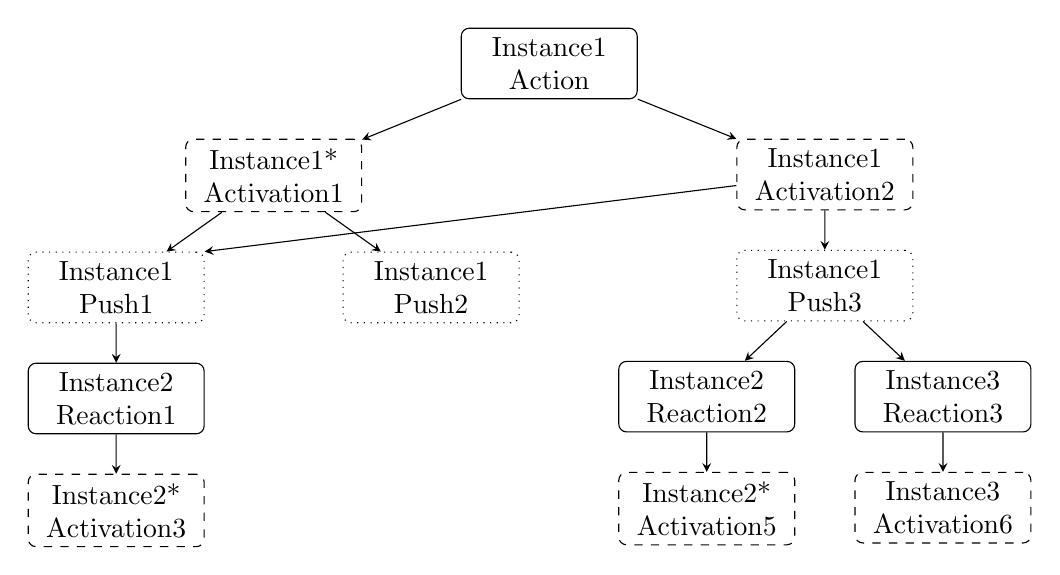
\begin{tikzpicture}[
    arrowstyle/.style={draw, -stealth},
    edge from parent/.style={draw, -stealth},
    reaction/.style={rectangle, draw, rounded corners=1mm, text width=2cm,
        text centered, anchor=north},
    activation/.style={rectangle, draw, rounded corners=1mm, dashed, text width=2cm,
        text centered, anchor=north},
    push/.style={rectangle, draw, rounded corners=1mm, dotted, text width=2cm,
        text centered, anchor=north},
    level 1/.style={sibling distance=7.0cm},
    level 2/.style={sibling distance=4.0cm},
    level 3/.style={sibling distance=3.0cm},
    level distance=0.5cm, growth parent anchor=south
]
\node (Action) [reaction] {Instance1 Action}
  child {
    node (Activation01) [activation] {Instance1* Activation1}
    child {
      node (Push01) [push] {Instance1 Push1}
      child {
        node (Reaction01) [reaction] {Instance2 Reaction1}
        child {
          node (Activation03) [activation] {Instance2* Activation3}
        }
      }
    }
    child {
      node (Push02) [push] {Instance1 Push2}
    }
  }
  child {
    node (Activation02) [activation] {Instance1 Activation2}
    child {
      node (Push03) [push] {Instance1 Push3}
      child {
        node (Reaction02) [reaction] {Instance2 Reaction2}
        child {
          node (Activation04) [activation] {Instance2* Activation5}
        }
      }
      child {
        node (Reaction03) [reaction] {Instance3 Reaction3}
        child {
          node (Activation05) [activation] {Instance3 Activation6}
        }
      }
    }
  }
;

\draw[arrowstyle] (Activation02) -- (Push01.north east);

\end{tikzpicture}
\endgroup
%%}%
\caption{Example transaction\label{transaction}}
\end{figure}

A recursive transaction is formed when a reaction activates itself through the set of bindings or a getter calls itself, which appears as a cycle in the transaction graph.
The \rcgo{} interpreter uses an implementation of Tarjan's algorithm~\cite{tarjan1976} to detect cycles.

A non-deterministic transaction occurs when the same state is manipulated by multiple transitions.
Thus, the interpreter must determine what state is manipulated in a transaction to determine if the constituent transitions are compatible.
The interpreter uses a component instance as a proxy for its state variables and determines how the state is accessed in each transition.
The possible access patterns include:
\begin{description}
  \item[Write] in which at least one state variable may be mutated (* in Figure~\ref{transaction});
  \item[Read] in which at least one state variable is accessed but no state variables are mutated; and
  \item[None] in which no state variables are accessed.
\end{description}
The current implementation uses a conservative static analysis of the body of an activate statement to determine if the activation mutates the state of the component.
For composition analysis, state variable access need only be determined for the mutable phase.
However, performing a similar analysis for the immutable phase and precondition provides a complete description of state access in a transaction, which is used by multi-threaded schedulers to determine which transactions can be executed in parallel.

The check for non-deterministic transactions continues by confirming that all possible executions of a transaction are deterministic in two steps.
First, two \emph{access sets} are computed for each node in the transaction.
The first access set describes what state is accessed in the immutable phase, while the second set describes what state is accessed in the mutable phase.
Let $W = \{ \mathit{Read}, \mathit{Write} \}$ be the set of relevant access patterns\footnote{The $\mathit{None}$ access pattern is intentionally ignored as an optimization.}.
Each element in an access set $h \in H$ is a pair $(i,w)$ where $i \in I$ and $w \in W$.
Let $\mathit{inst}: A \cup R \cup G \to I$ be a function that maps an action, reaction, or getter to the corresponding instance.
The immutable phase access sets are computed as follows:
\begin{itemize}
  \item For an action, reaction, or getter denoted as $x$ with instance $i = \mathit{inst}(x)$ that reads the state of $i$, the immutable phase access set is the union of the immutable phase access sets of its children and the set $\{ (i, \mathit{Read}) \}$.
  \item Otherwise, the immutable phase access set is just the union of the immutable phase access sets of its children.
\end{itemize}
The mutable phase access sets are computed as follows:
\begin{itemize}
  \item If the node is not an activation, or is an activation that does not access the state of the instance, then the mutable phase access set is the union of the mutable phase access sets of its children.
  \item Otherwise, the node is an activation belonging to instance $i \in I$ with access $w \in W$ and the mutable phase access set is the union of the mutable phase access sets of its children and $\{ (i, w) \}$.
\end{itemize}
The access sets for the root of a transaction describe how state may be accessed during each phase of the transaction.
An analysis similar to the immutable phase analysis may be applied to the precondition.
All access pairs in the precondition and immutable phase access sets have $\mathit{Read}$ access.
Access pairs in the mutable phase access sets may either have $\mathit{Read}$ or $\mathit{Write}$ access.
Activate statements that do nothing but log the state of a component are a common example of mutable phase access pairs with $\mathit{Read}$ access.

\begin{figure}
\centering
%%\resizebox{\textwidth}{!}{%
\begingroup
\fontsize{10pt}{12pt}\selectfont
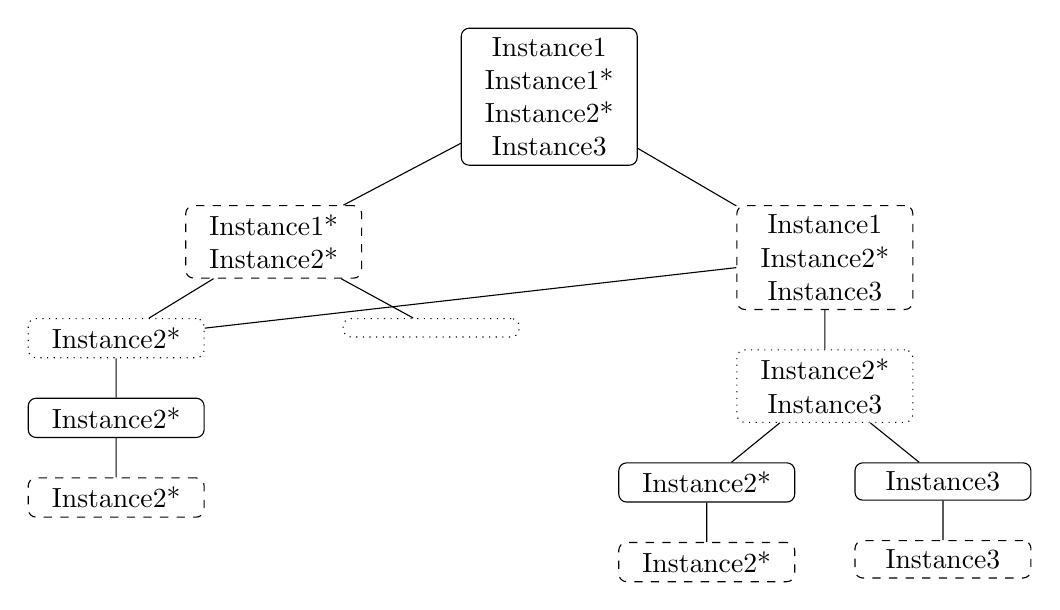
\begin{tikzpicture}[
    reaction/.style={rectangle, draw, rounded corners=1mm, text width=2cm,
        text centered, anchor=north},
    activation/.style={rectangle, draw, rounded corners=1mm, dashed, text width=2cm,
        text centered, anchor=north},
    push/.style={rectangle, draw, rounded corners=1mm, dotted, text width=2cm,
        text centered, anchor=north},
    level 1/.style={sibling distance=7.0cm},
    level 2/.style={sibling distance=4.0cm},
    level 3/.style={sibling distance=3.0cm},
    level distance=0.5cm, growth parent anchor=south
]
\node (Action) [reaction] {Instance1 Instance1* Instance2* Instance3}
  child {
    node (Activation01) [activation] {Instance1* Instance2*}
    child {
      node (Push01) [push] {Instance2*}
      child {
        node (Reaction01) [reaction] {Instance2*}
        child {
          node (Activation03) [activation] {Instance2*}
        }
      }
    }
    child {
      node (Push02) [push] {}
    }
  }
  child {
    node (Activation02) [activation] {Instance1 Instance2* Instance3}
    child {
      node (Push03) [push] {Instance2* Instance3}
      child {
        node (Reaction02) [reaction] {Instance2*}
        child {
          node (Activation04) [activation] {Instance2*}
        }
      }
      child {
        node (Reaction03) [reaction] {Instance3}
        child {
          node (Activation05) [activation] {Instance3}
        }
      }
    }
  }
;

\draw (Activation02) -- (Push01);

\end{tikzpicture}
\endgroup
%%}%
\caption{Example mutable phase access set calculation\label{access_sets}}
\end{figure}

Figure~\ref{access_sets} shows the mutable phase access set calculation for the transaction illustrated in Figure~\ref{transaction}.
The root shows that Instance1 does not change in at least one activation (Instance1) and may change in at least one activation (Instance1*), that Instance2 may change in every activation (Instance2*), and that Instance3 is read-only in this transaction (Instance3).
The empty node in Figure~\ref{access_sets} comes from an unbound push port.

The second step for detecting a non-deterministic transaction is to verify that a mutated instance appears in at most one child node access set for the activation and push port nodes.
Let $\mathit{race}: \{ H \} \times \{ H \} \to \mathcal{B}$ be a predicate that indicates a data race between two access sets.
This function is defined as follows:
\begin{multline}
  \mathit{race} (H_1, H_2) = \\
  (\exists i : (i, \mathit{Write}) \in H_1 \land (i, x) \in H_2) \lor
  (\exists j : (j, \mathit{Write}) \in H_2 \land (j, y) \in H_1)
\end{multline}
This is, a component that changes state in one access set may not appear in the other access set.
The $\mathit{race}$ predicate is computed for each pair of child mutable phase access sets in activation and push port nodes.
This check succeeds everywhere but Activation2 in Figures~\ref{transaction}~and~\ref{access_sets}, as Instance2* appears in both children.
The activation and push port nodes represent activities that will be performed together.
That is, once control passes to an activate statement, all push ports and their bound reactions are activated.
In contrast, activations (as children of action and reaction nodes) represent mutually exclusive alternatives:  at most one activate statement is executed per action/reaction body.
Thus, a mutated instance appearing in two or more children of an activation node or push port node indicates that the state of a component may be mutated in disparate ways leading to a non-deterministic transaction.

\paragraph{Complexity.}
Maintaining appropriate forward and reverse hash maps of the bindings allows the binding check to be performed in $O(N)$ time where $N$ is the number of ports in the system.
Similarly, the construction of a transaction graph can be performed in $O(|N| + |V|)$ time where $|N|$ is the number of nodes in the transaction and $|V|$ is the number of edges.
Proving that a transaction is acyclic can be performed in $O(|N| + |V|)$ time where $|N|$ is the number of nodes and $|V|$ is the number of edges.

A loose upper-bound on the complexity of the access set calculations for the non-determinism check is $O(k |N|^2 \log (|N|))$ where $|N|$ represents the number of nodes in a transaction and $k$ represents the maximum branching factor in the transaction.
The size of the access set for the root is $|N|$.
Assuming a naive set implementation, the complexity of computing the access set for the root is $O(|N| \log (|N|))$.
This must be repeated $k$ times for all nodes in the graph resulting in an overall complexity of $O(k |N|^2 \log (|N|))$.

A loose upper-bound on the complexity of the compatibility check is also $O(k |N|^2 \log (|N|))$.
Assume that the size of the access set at each node is $|N|$.
A tree-based set lookup can be performed in $O(\log(|N|))$ time.
The lookup must be performed $k |N|$ times by the parent.
The lookup must repeated for each of the $|N|$ nodes for a combined complexity of $O(k |N|^2 \log (|N|))$.

The complexity of these algorithms has not presented a problem in practice as most of the systems we have implemented have small numbers for $|N|$, $|V|$, and $k$.

\section{Activations}
\label{activations}

When executing a transaction, the \rcgo{} run-time system must execute the immutable phase of all implied state transitions before executing any of the mutable phases.
To accomplish this, the run-time system uses a novel calling convention to create a list of deferred contexts and statements that represent the mutable phase of each state transition.
The immutable phase constructs the list and the mutable phase processes the list.
To present the calling convention, we first present some details about the run-time system such as the ordinary calling convention and push ports.
We then describe the behavior of the calling convention and explain it using an illustrative example.

\paragraph{Ordinary calling convention.}
The ordinary call mechanism in the \rcgo{} run-time system is similar to the C-decl calling convention.
It assumes the existence of an \emph{instruction pointer}, which contains the address of the currently executing instruction, and a \emph{base pointer} that points to a location in the stack, which can be offset to access arguments and local variables.
An ordinary call in the language is accomplished through the following sequence:
\begin{enumerate}
\item (Caller) Create space for return values.
\item (Caller) Push arguments onto the stack, left to right.
\item (Caller) Push the instruction pointer onto the stack and transfer control to the body of the function, method, action, reaction, getter, or initializer.
\item (Callee) Push the base pointer onto the stack and set the base pointer to the top of the stack.
\item (Callee) Reserve space on the stack for local variables.
\item (Callee) Execute the body of the function, method, etc.
\item (Callee) Pop the stack, pop and restore the base pointer, pop and restore the instruction pointer.
\item (Caller) Pop the arguments.
\item (Caller) Pop the return values.
\end{enumerate}
The major difference between this calling convention and C-decl is that the arguments are pushed in the opposite order to match the semantics of Go.
The collection of arguments, previous instruction pointer, previous base pointer, and reserved space is called a \emph{stack frame} (or \emph{call frame}).
Figure~\ref{frame} shows the layout of a normal stack frame.
For this presentation, we assume that the stack grows down, i.e., the previous base pointer has a lower address in memory than the previous instruction pointer.

\begin{figure}
\centering
\resizebox{.5\textwidth}{!}{%
\begingroup
\fontsize{10pt}{12pt}\selectfont
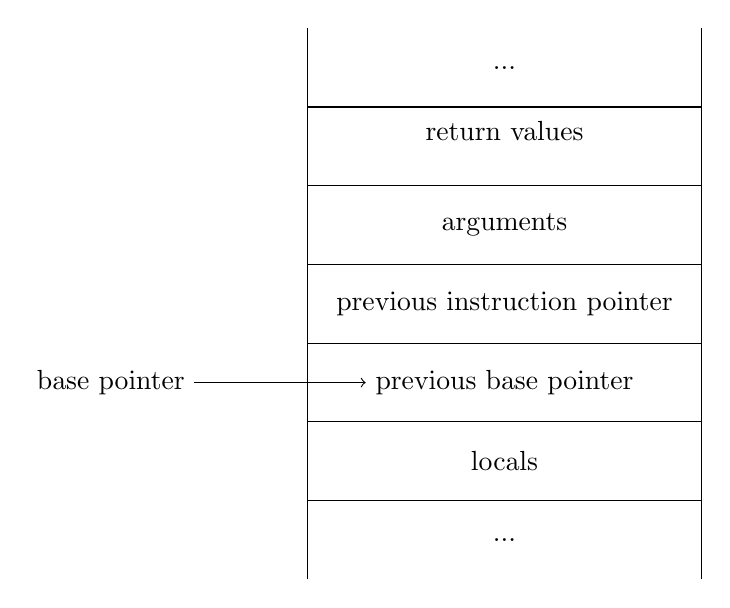
\begin{tikzpicture}
%% component boundary

\draw (0,1) -- (0,8);
\draw (5,1) -- (5,8);

\node at (2.5, 7.5) { ... };
\draw (0,7) -- (5, 7);
\node at (2.5, 6.7) { return values };
\draw (0,6) -- (5,6);
\node at (2.5, 5.5) { arguments };
\draw (0,5) -- (5,5);
\node at (2.5, 4.5) { previous instruction pointer };
\draw (0,4) -- (5,4);
\node (pbp) at (2.5, 3.5) { previous base pointer };
\draw (0,3) -- (5,3);
\node at (2.5, 2.5) { locals };
\draw (0,2) -- (5,2);
\node at (2.5, 1.5) { ... };

\node (bp) at (-2.5, 3.5) { base pointer };
\draw[->] (bp) -- (pbp);

\end{tikzpicture}
\endgroup
}%
\caption[Diagram of a stack frame]{Diagram of a stack frame.  The stack is depicted as growing down.}
\label{frame}
\end{figure}

\paragraph{Push ports.}
A push port is a field in a component, which is implemented as a pointer to a linked list that contains the component pointer/reaction pairs that are bound to the push port.
The \rcgo{} run-time system populates each push port before execution begins.

\paragraph{Synchronized two-phase calling convention.}
As was previously stated, the execution of an activate statement is split into an immutable phase and a mutable phase.
To prepare for the mutable phase, the immutable phase must preserve the stack frame (context) of the action or reaction that executes an activate statement and must record which activate statement was executed so that the same activation can be resumed in the mutable phase.
To accomplish this, we devised a \emph{synchronized two-phase calling convention}, which is used to execute activate statements during the immutable phase.

Recall that activate statements may only appear in actions and reactions.
After executing the immutable phase of an activate statement in a reaction, control must be returned to the calling activate statement so that it may activate other push ports.
After executing the immutable phase of an activate statement in an action, control must be returned to the \rcgo{} run-time system to begin the mutable phase.

In the ordinary calling convention, the stack frame for the reaction would be popped, control would be returned to the caller, and the arguments would be popped.
To preserve the stack frame for use during the mutable phase, however, the activate statement returns control to the caller without popping the frame and the caller does not pop the arguments.
Thus, the complete frame for the reaction is preserved on the stack.

Each such deferred stack frame is added to a list to make it available in the mutable phase.
Let $head$ be a variable containing a pointer, initially nil, which will serve as the head of a linked list.
Before the activate statement returns from the immutable phase, it sets the previous base pointer in the deferred stack frame to the value of $head$ and updates head to be the current base pointer which inserts the stack frame into the list.
The \rcgo{} run-time system can iterate over the elements of the list by following the previous base pointer to access all of the stack frames that are needed for the mutable phase.
If the list is empty ($head$ is nil), then no activate statement was executed and the mutable phase may be skipped.

The final piece of information that must be recorded is the body of the activate statement so that it is accessible in the mutable phase.
Before returning from the immutable phase, the activate statement records the body of the activate statement in the previous instruction pointer slot of the current stack frame.
It is safe to use the previous instruction pointer because it is not used beyond the immediate return.
Furthermore, it is at a fixed location, which allows it to be accessed in any deferred stack frame.

The synchronized two-phase calling convention is used when executing an activate statement and proceeds as follows:
\begin{enumerate}
\item Save the previous base pointer of the current stack frame in $bp$.
\item Set the previous base pointer of the current stack frame to the value of $head$.
\item Set $head$ to the value of the base pointer.
\item Save the previous instruction pointer of the current stack frame in $ip$.
\item Set the previous instruction pointer of the current stack frame to the body of the activate statement.
\item For each push port in the port call list:
  \begin{enumerate}
  \item Push the arguments to the push port onto the stack.\label{step1}
  \item For each component pointer/reaction pair in the push port:
    \begin{enumerate}
    \item Push the component pointer onto the stack.
    \item Copy the arguments prepared in~\ref{step1} onto the stack.
    \item Call the reaction.
    \end{enumerate}
  \end{enumerate}
\item Set the base pointer to the value of $bp$ and return control to the address in $ip$.
\end{enumerate}

The synchronized two-phase calling convention evaluates the arguments to a push port once and passes a copy to each bound reaction.
An alternative would be to evaluate the arguments for each bound reaction.
This means that the arguments may not be evaluated (i.e., the push port is not bound to any reactions) or may be evaluated multiple times.
If the arguments contain an expression with side-effects, then the behavior of the code becomes dependent on composition.
While this may be desirable in some cases, we opted for making a port call resemble an ordinary function call as much as possible.
This sentiment also influenced our decision to pass a copy of the arguments to each reaction as opposed to reusing the same set of prepared arguments.
Since each reaction starts with a copy of the arguments, it is free to manipulate them as allowed by the semantics of Go.
Furthermore, the arguments are available in the mutable phase which obviates the need to make local copies of arguments.
This approach assumes that copying arguments does not generate significant overhead.

%% After an activate statement calls the last push port, it makes temporary copies of the instruction pointer and base pointer of the caller.
%% It may then safely overwrite the base pointer to insert itself into the list of mutable phase stack frames and it may safely overwrite the instruction pointer with the body of the activate statement.

A major caveat when using the synchronized two-phase calling convention is that it must be assumed that the stack pointer changes when calling a push port.
To illustrate why this is an issue, consider the case when a caller wishes to preserve the contents of a register.
One strategy is to push the contents of the register onto the stack, perform the call, and then pop the value from the stack into the register.
After calling a push port, the caller may no longer assume that the previous value of the register is at the top of the stack.
An easy work-around is to allocate local variables, i.e., variables whose addresses are relative to the base pointer instead of the stack pointer, for saving temporary values that must persist across a push port call.
In the same way, the variables used to iterate over the list of component/reaction pairs in a push port should be allocated as local variables so that they may survive the calls to the reactions.

\paragraph{Mutable phase.}
The mutable phase consists of executing all of the deferred activate statements.
The algorithm for doing so is as follows:
\begin{enumerate}
\item If the value of $head$ is nil, stop.  Otherwise, set the base pointer to the value in $head$.
\item Transfer control to the instruction indicated by the previous instruction pointer\label{transfer}.  Execution continues until the body of the activate statement (implicitly or explicitly) returns.
\item If the previous base pointer is nil, stop.  Otherwise, set the base pointer to the previous base pointer and go to \ref{transfer}.
\end{enumerate}

The algorithm iterates over the list of deferred stack frames accessible through $head$.
The last element in the list is indicated by a previous base pointer that is nil.
Control is transferred to the previous instruction pointer which contains the body of the activate statement.

\begin{figure}
\centering
\resizebox{.75\textwidth}{!}{%
\begingroup
\fontsize{10pt}{12pt}\selectfont
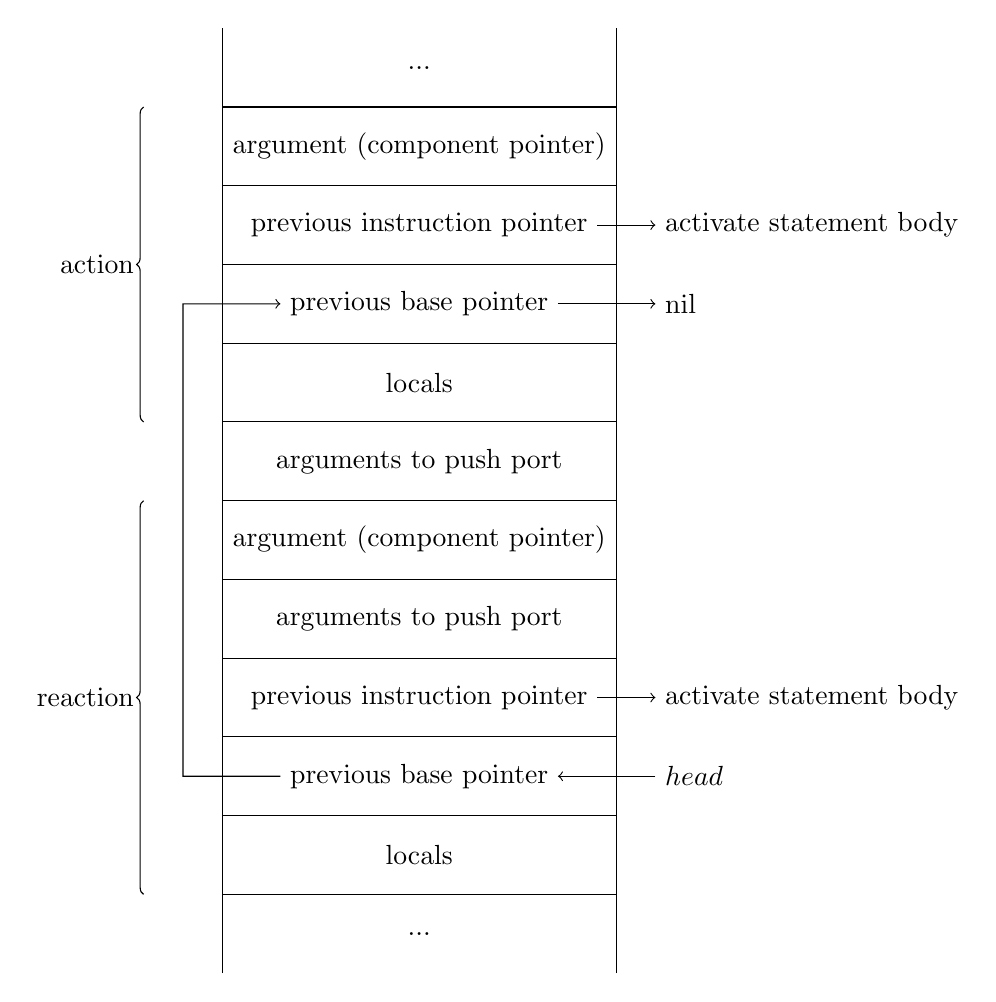
\begin{tikzpicture}
%% component boundary

\draw (0,-5) -- (0,7);
\draw (5,-5) -- (5,7);

\node at (2.5, 6.5) { ... };
\draw (0,6) -- (5,6);
\node at (2.5, 5.5) { argument (component pointer) };
\draw (0,5) -- (5,5);
\node (pip1) at (2.5, 4.5) { previous instruction pointer };
\draw (0,4) -- (5,4);
\node (pbp1) at (2.5, 3.5) { previous base pointer };
\draw (0,3) -- (5,3);
\node at (2.5, 2.5) { locals };
\draw (0,2) -- (5,2);
\node at (2.5, 1.5) { arguments to push port };
\draw (0,1) -- (5,1);
\node at (2.5, .5) { argument (component pointer) };
\draw (0,0) -- (5,0);
\node at (2.5, -.5) { arguments to push port };
\draw (0,-1) -- (5,-1);
\node (pip2) at (2.5, -1.5) { previous instruction pointer };
\draw (0,-2) -- (5,-2);
\node (pbp2) at (2.5, -2.5) { previous base pointer };
\draw (0,-3) -- (5,-3);
\node at (2.5, -3.5) { locals };
\draw (0,-4) -- (5,-4);
\node at (2.5, -4.5) { ... };

\node[anchor=west] (as1) at (5.5, 4.5) { activate statement body };
\draw[->] (pip1) -- (as1);
\node[anchor=west] (as2) at (5.5, -1.5) { activate statement body };
\draw[->] (pip2) -- (as2);

\draw[->] (pbp2) -- ++(-3,0) -- ++(0,6) -- (pbp1);

\node[anchor=west] (nil) at (5.5, 3.5) { nil };
\draw[->] (pbp1) -- (nil);

\node[anchor=west] (head) at (5.5, -2.5) { $head$ };
\draw[->] (head) -- (pbp2);

\draw[decorate,decoration={brace}] (-1,2) -- (-1,6) node[anchor=east,midway] { action };

\draw[decorate,decoration={brace}] (-1,-4) -- (-1,1) node[anchor=east,midway] { reaction };

\end{tikzpicture}
\endgroup
}%
\caption[Diagram of the stack after the immutable phase for single action-reaction]{Diagram of the stack after the immutable phase when an action activates a single reaction}
\label{activation_ex_1}
\end{figure}

\paragraph{Example:  one action, one reaction.}
Suppose an action activates a single push port that is bound to a single reaction and the reaction has a single activation that does not activate any push ports.
Figure~\ref{activation_ex_1} shows a diagram of the stack after the immutable phase for this scenario.
The stack contains two frames, one corresponding to the action and one corresponding to the reaction.
The $head$ variable points to the reaction frame which in turn points to the action frame using the previous base pointer slot.
The action frame points to nil indicating that it is the last frame in the list.
The previous instruction pointers point to the bodies of the activate statements.
Between the frames are the push port arguments which are duplicated for the call to the reaction.
If the push port had been bound to multiple reactions, then the reaction portion of the diagram would be replicated to match the number of bound reactions.
If multiple push ports were activated by the activate statement, then additional push port arguments and reactions would appear on the stack.

\paragraph{Calling convention efficiency.}
The synchronized two-phase calling convention has the potential to be as efficient as a function or method call.
The proposed calling convention can be implemented directly on modern hardware architectures like x86 and x86\_64, which contain all of the registers and instructions necessary to support the synchronized two-phase calling convention.
The synchronized two-phase calling convention relies solely on the stack which means that the underlying operating system must set up the stack, back it with memory pages, etc.
More importantly, it avoids the overhead of heap allocation.
Port calls resemble virtual method calls in that the reactions may need to be looked up before they can be executed.
However, this lookup could be avoided by inlining the body of each reaction using the substitutional equivalence property.
This could be performed prior to execution or during execution using just-in-time compilation techniques.
We leave the application of these techniques to future work.

\section{Heaps}
\label{heaps}

In this section, we describe the implementation of the heap data type introduced in Chapter~\ref{language} and our approach to garbage collection.
Our approach to implementing dynamic memory allocation and garbage collection was shaped by the independence of state required by the semantics of reactive components.
Thus, instead of relying on a single global heap, the implementation contains a heap for each component that can be garbage collected independently of the others.
This independence allows garbage collection to be performed concurrently with other activities using simple, single-threaded algorithms.

\paragraph{Slots and blocks.}
A \emph{slot} is the smallest unit of memory that can be dynamically allocated.
Typically, a slot is the size of two pointers.
A \emph{block} is an extent of memory and a set of bits indicating the allocation status of each slot in the extent.
The status bits indicate if a slot is allocated, if a slot is the beginning of an object, and if the slot has been marked by the mark-and-sweep algorithm.
Blocks also contain left and right pointers that allow them to be formed into a binary tree ordered by the address of the extent.

\paragraph{Mark-and-sweep garbage collection.}
We implemented a simple mark-and-sweep algorithm to collect garbage in a tree of blocks.
The core of the marking phase involves scanning extents for pointers to objects.
When the algorithm comes across a slot that is allocated, marked, and which contains a pointer-sized value that points to a location in the tree of blocks that is also allocated, it marks the object indicated by the pointer.
The algorithm is bootstrapped by marking all slots in a designated root object.
The algorithm repeatedly scans the extents in the tree of blocks until no new marks can be added.
At this point, the sweep phase resets the allocated bit for all slots that are allocated but not marked and resets the marked bit for the next run of the algorithm.
A block that is not marked, meaning that none of its slots were marked, is removed from the tree of blocks and deallocated.

\paragraph{Heaps.}
A \emph{heap} contains a root block, a list of unallocated chunks of memory (free list), and pointers to create a tree structure.
When allocating an object from a heap, the heap attempts to find an adequate chunk in the free list using a first-fit policy.
If this fails, the heap allocates a new block, inserts it into the tree and free list, and then allocates again using the newly inserted chunk.
The sweep phase of the mark-and-sweep algorithm reconstructs the free list.

As described in Chapter~\ref{language}, every component has an associated heap.
A heap of this kind is called an \emph{implicit heap}.
Heaps that are created via \verb+new+ and passed to \verb+move+, \verb+merge+, and \verb+change+ are called \emph{explicit heaps}.
All heaps have a distinguished root object.
The marking phase of the mark-and-sweep algorithm is seeded with this root object.
The root object of an implicit heap contains the statically allocated state of the component that owns the heap.
The root object of an explicit heap is an object that is allocated in the same heap.

The semantics of reactive components allow heaps to form strict hierarchies, i.e., a tree structure where the root of the tree is an implicit heap and the internal nodes and leaves of the tree are explicit heaps.
A strict hierarchy gives a graphical interpretation to merge and move operations.
A move operation moves a sub-tree from one location to another location.
 Merging a heap $h$ into another heap $p$ involves removing $h$ from the tree, inserting the blocks of $h$ into the tree of blocks of $p$, merging the free list of $h$ into the free list of $p$, and inserting the children of $h$ as children of $p$.

\paragraph{The active heap.}
Logically, the \rcgo{} run-time system maintains a stack of heaps where the top of the stack represents the \emph{active heap}.
The active heap is used to satisfy all dynamic memory requests, i.e., calls to \verb+new+.
The implicit heap that is associated with the receiving component is pushed/popped upon entering/leaving an action, reaction, getter, or initializer.
Specific \verb+change+ statements are used to push and pop explicit heaps.
Thus, the call stack (i.e., the \verb+change+ statements that are active on the call stack) implements the stack of heaps.
When a new heap is created, it is inserted as a child of the active heap.

\paragraph{Atomicity.}
Chapter~\ref{language} describes how the semantics of reactive components permit concurrent access to heaps.
The first scenario where this may occur is when a heap is passed to a push port that is bound to multiple reactions.
The semantics of reactive components allow the reactions to be executed concurrently.
Thus, two different threads may attempt to move/merge the same heap at the same time.
The second scenario occurs when a component is concurrently accessed in multiple transactions that don't mutate the state of the component.
The action, reaction, or getter is allowed to allocate memory, which means that heaps must correctly handle concurrent access.
Our implementation of heaps uses the Thread Safe Interface pattern~\cite{schmidt2000pattern} to synchronize access to heaps when allocating, moving, and merging.

\paragraph{Heap links.}
Heaps are exposed to users via pointers to heaps, e.g., \verb+*heap int+.
These pointers to heaps can be stored in objects allocated in another heap.
The semantics of \verb+change+, \verb+merge+, and \verb+move+ ensure that the parent-child relationships formed by pointers to heaps match exactly those known by the run-time system.
The two rules that enforce this behavior are that 1) \verb+merge+ and \verb+move+ fail for any heap that is already on the stack of active heaps and 2) all pointers in scope become foreign in the body of a change statement.
The second rule forces the user to \verb+move+ heaps if they desire to change the hierarchy, because pointers with foreign indirection mutability cannot be stored.
Recall that the stack of active heaps is set up by active \verb+change+ statements.
Using the inductive argument that the parent-child relationship was previously correct, then the ancestors of the active heap must all appear in the stack of active heaps.
Thus, failing to \verb+merge+ and \verb+move+ heaps on the active stack prevents the formation of cycles.

\begin{figure}
\centering
%%\resizebox{\textwidth}{!}{%
\begingroup
\fontsize{10pt}{12pt}\selectfont
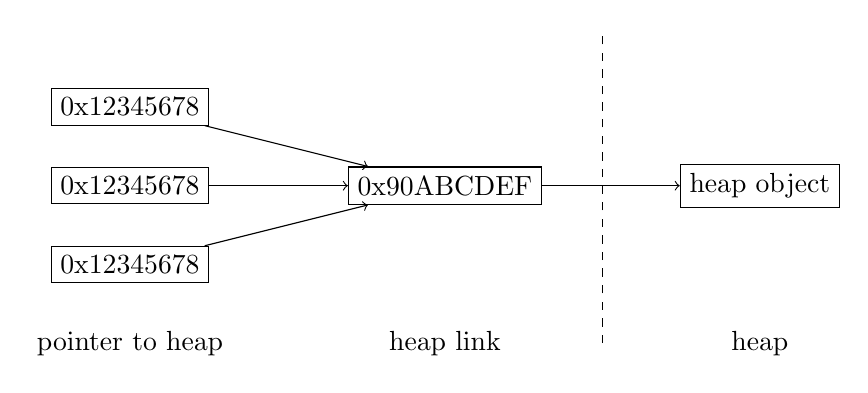
\begin{tikzpicture}
\node [rectangle, draw] (p1) at (0,1) {0x12345678};
\node [rectangle, draw] (p2) at (0,0) {0x12345678};
\node [rectangle, draw] (p3) at (0,-1) {0x12345678};
\node at (0,-2) {pointer to heap};
\node [rectangle, draw] (hl) at (4,0) {0x90ABCDEF};
\node at (4,-2) {heap link};
\node [rectangle, draw] (heap) at (8,0) {heap object};
\node at (8,-2) {heap};
\draw [->] (p1) -- (hl);
\draw [->] (p2) -- (hl);
\draw [->] (p3) -- (hl);
\draw [->] (hl) -- (heap);
\draw [dashed] (6, -2) -- (6, 2);
\end{tikzpicture}
\endgroup
%%}%
\cprotect\caption[Heap link example]{Example illustrating heap links.  The objects on the far left represent user-level pointers to heaps, e.g., \verb+* heap int+.  The middle object is a heap link, which contains the address of the child heap that appears on the far right.}
\label{heap_link}
\end{figure}

As illustrated in Figure~\ref{heap_link}, a user-level pointer to a heap points to an object called a heap link which in turn points to a heap.
The objects on the left side of the diagram are objects in the parent heap and the object on the right is the child heap.
The extra level of indirection introduced by the heap link concentrates all references to the child heap into one location.
Moving a heap involves reading the pointer out of the heap link and replacing it with \verb+nil+.
This makes the heap inaccessible to the previous owner (parent), which maintains the isolation of state between reactive components.
The marking phase of the mark-and-sweep algorithm is aware of heap links and marks heaps as being reachable from another heap.
Unreachable heaps are pruned from the hierarchy during garbage collection.

\paragraph{Concurrent garbage collection.}
Two features of reactive components permit concurrent garbage collection.
First, the state of each reactive component is isolated which allows garbage collection to be performed on different components at the same time without conflict.
Second, garbage collection can be framed as an action to be executed by the scheduler.
Thus, associated with each component is an action that invokes the garbage collector on the implicit and explicit heaps of the corresponding component.
Furthermore, the action is considered to modify the state of the component which prevents all transactions involving the component from executing concurrently with the garbage collection action.
We assume that the scheduler executes the garbage collection action often enough that no additional invocations of the garbage collector are necessary.
More plainly, we do not trigger the garbage collector in the allocation routine, which is the approach taken by many systems using garbage collection.
Most garbage collection algorithms include a scan of the call stack as objects reachable from the call stack must not be collected.
In our approach, such scanning is useless since the call stack is empty when executing the garbage collection action and the root object is embedded in the implicit heap that is being collected.

\section{I/O}

A possible bottom-up approach to support reactive components would be to write a kernel for reactive components, i.e., a scheduler and memory manager, and then write an operating system and application suites using reactive components.
This approach, however, is impractical and risky given the expense of developing software for an as yet unproven technology.
A top-down approach instead involves proving the utility of reactive components at the application layer and then proceeding to lower layers when appropriate.
This approach far less risky and is the one taken in this chapter.
To develop and evaluate real-world applications, the input/output facilities of the host operating system then must be exposed to reactive components so that they may communicate and interact with other processes and systems.
This section describes our approach to exposing the input/output (I/O) facilities of a Linux/GNU system to reactive components.

A Linux/GNU system offers a variety of I/O and communication mechanisms including pipes, sockets, shared memory, and message queues.
For our purposes, we focused on mechanisms that are available through a file descriptor interface.
Our approach consists of two steps.
The first step is to add file descriptors and operations for manipulating them, such as read and write, to the \rcgo{} language.
The second step was to wrap file descriptors in reactive components to make their functionality available via a conventional reactive component interface.

The main consideration when supporting file descriptors was to ensure that reads and writes were non-blocking, as a blocking read or write may violate fairness.
A transaction that blocks on a read or write would adversely affect the latency and throughput of the scheduler as the scheduler thread would be blocked and not able to service other transactions.
Furthermore, a blocking transaction holds the locks for all components involved in that transaction, and other enabled transactions that also involve those components would be denied service which also violates the fairness requirement of the scheduler.
To prevent these problems, all file descriptors when they are created are set to be non-blocking.
Thus, all subsequent reads and writes are also non-blocking.

Threaded programs using non-blocking I/O typically use some kind of synchronous I/O multiplexing which allows a thread to determine which file descriptors are ready for reading and/or writing.
The goal in doing so is to allow a thread to service multiple file descriptors and yield the processor if no file descriptors are ready.
To map this concept into reactive components, we introduced a \verb+readable+ function that tests if a file descriptor is ready for reading and a \verb+writable+ function that tests if a file descriptor is ready for writing.
These functions are intended to be used in preconditions so that an action becomes enabled when the corresponding file descriptor is ready.

The \verb+readable+ and \verb+writable+ functions are also used as part of the termination protocol of the Partitioned scheduler described in Section~\ref{scheduler_implementation}.
When the termination protocol enters the checking phase where it attempts to prove that every precondition is false, it records which file descriptors are being checking for readability and writability.
If the termination protocol proves that all preconditions are false but some preconditions depend on readability or writability, it enters a state where it waits for one of the file descriptors to become ready.
This allows a system of reactive components to sleep while it waits for external input like a message from a remote host or a timer.

Conceptually, a file descriptor contains component state and should be subject to all of the constraints of normal component state.
The two main constraints are 1) it cannot be shared by another component and 2) it cannot change in the immutable phase of a transaction.
To enforce the first constraint, file descriptors are implemented as dynamically allocated opaque data structures.
Forcing dynamic allocation makes file descriptors subject to the pointer sharing rules, i.e., they can only be shared via foreign indirection mutability in the immutable phase.
Making the data structure opaque prevents sharing through copying.
The normal immutable phase rules in concert with properly declared built-in functions prevent file descriptors from changing in the immutable phase.
That is, functions like \verb+read+ and \verb+write+ require a pointer to a file descriptor with mutable indirection mutability.

To test these ideas, we implemented a Simple Network Time Protocol (SNTP) client.
SNTP attempts to acquire the current time from a server while simultaneously measuring a round-trip latency to determine an accurate local time.
The client timestamps the request with the local time and sends it to the server.
The server timestamps the request when it arrives and again when it sends it back to the client.
Finally, the client timestamps the request when it receives it back from server.
The client uses the timestamps to determine the offset of the local clock from the clock on the server.
This procedure is repeated periodically to synchronize the local clock.
The messages are exchanged using the User Datagram Protocol (UDP).

\begin{figure}
\centering
\resizebox{\textwidth}{!}{%
\begingroup
\fontsize{10pt}{12pt}\selectfont
\begin{tikzpicture}
\draw (2,7.5) rectangle (4,9);
\node[below] at (3,9) {Timer};
\rapush[4,8,1.8,.5,alarma,ignore]{Alarm()};

\draw (1.5,6) rectangle (16.5,10);
\node[below] at (8.5,10) {Sntp};
\lppush[5,8,1.8,.5,alarmb,ignore]{Alarm()};
\rapush[11,8,3.5,.5,senda,ignore]{Send(UdpMessage)};
\rppush[11,7,4.1,.5,receivea,ignore]{Receive(UdpMessage)};

\draw (12,6.5) rectangle (16,9);
\node[below] at (14,9) {UdpParticipant};
\lppush[12,8,3.7,.5,sendb,ignore]{Send(UdpMessage)};
\lapush[12,7,3.8,.5,receiveb,ignore]{Receive(UdpMessage)};

\draw (alarma.center) -- (alarmb.center);
\draw (senda.center) -- (sendb.center);
\draw (receivea.center) -- (receiveb.center);

\end{tikzpicture}
\endgroup
}%
\caption{Diagram of a Simple Network Time Protocol (SNTP) client\label{sntp}}
\end{figure}

Figure~\ref{sntp} shows a diagram of the SNTP client application.
The top-level Sntp component contains two sub-components:  Timer and UdpParticipant.
The Timer component is a periodic timer implemented by wrapping a \verb+timerfd+ file descriptor.
The UdpParticipant component wraps a UDP socket file descriptor and is capable of sending and receiving UDP messages.
The Sntp component uses these components to implement an SNTP client.
Whenever the Timer fires the alarm, the UdpParticipant creates an SNTP request and sends it using the UdpParticipant.
This all happens as part of one atomic transaction.
Whenever the UdpParticipant receives a message, it passes it to the Sntp component which deserializes it, timestamps it, and interprets it to compute the local clock offset.

The Sntp component demonstrates how composition (with reactive components for I/O) can be used to construct systems.
The Timer and UdpParticipant components are generic since they do not contain any SNTP related logic.
Furthermore, they have well-defined concurrency semantics that will be enforced when they are composed in other systems.
Thus, it is possible to use the reactive component model to produce reusable \emph{reactive} software.

\section{Summary}

The goal of implementing reactive components was to test the practicality of the reactive component model.
Specifically, we desired to know how the various features of the model could be implemented, which features were troublesome, and how the implementation utilizes various assumptions.
Flexibility in the reactive component model necessitates a check for sound composition.
The sound composition algorithm described in Section~\ref{sound_composition} uses the static system assumption and the component proxy assumption to generate a graphical model of each transition and check it for determinism.
A cursory analysis yielded an upper bound of $O(k n^2 \log (n))$ where $n$ is the number of instances involved in the transaction.

To implement activate statements, we developed the synchronized two-phase calling convention which executes the immutable phase of a transaction first and preserves the context necessary for the second (mutable) phase.
The synchronized two-phase calling convention was implemented using standard function call and stack manipulation facilities.

The isolation of component state is enforced in two ways.
First, the type system prevents components from sharing pointers directly via \verb+$const+ and \verb+$foreign+ modifiers.
Second, the implementation uses garbage collection to prevent indirect sharing through dangling pointers.
In this chapter, we describe the implementation of heaps and how they are used for dynamic memory allocation.
Heaps are designed so that they can be merged and moved.
At the user level, all references to a heap are encapsulated by a ``link'' which is used to enforce atomic moves and merges.
The independence of state between components allows each component to have its own heap (or tree of heaps) that can be garbage collected independently of other components.
Garbage collection can be conducted in parallel by associating a garbage collection action with each component.

To enhance the practicality of the reactive component implementation, we introduced file descriptor I/O that allows reactive components to interact with a variety of operating system facilities.
All I/O is non-blocking to preserve the fairness of the scheduler.
Components may use the \verb+readable+ and \verb+writable+ functions to test file descriptors.
The scheduler uses these functions as part of the termination protocol to sleep while waiting for external inputs.
File descriptors are treated as component state and therefore cannot be shared between components or mutated during the immutable phase.
Using file descriptor I/O, we implemented an SNTP client, which demonstrates how systems can be built up from simple components.

\chapter{Transaction Scheduler}
\label{scheduler}

A scheduler is responsible for executing transactions according to the fairness criteria set forth in Chapter~\ref{model}.
Of particular interest is the design and implementation of general-purpose schedulers that are capable of executing transactions in parallel.
The main inputs to a scheduler are the transactions enumerated by the composition analysis.
The access sets calculated for each transaction are used by concurrent schedulers to avoid non-deterministic state transitions.
In this chapter, we introduce some of the issues involved in designing and implementing a scheduler for reactive components, through a series of increasingly complex scheduler designs.
The two concrete implementations described later will draw upon the designs of these schedulers.

\section{The Transaction Scheduling Problem}
\label{scheduling_problem}

A scheduler is responsible for mapping transactions to processor cores so that they can be executed according to the semantics of reactive components.
As described in Chapter~\ref{model}, concurrent execution is modeled by a scheduler that serially and repeatedly executes atomic transactions according to fairness, which means that all enabled transaction must eventually be executed.
A scheduler implementation supporting concurrent execution must take care to preserve the fairness and atomicity required by the model.
A scheduler is \emph{fair} if it executes each transaction an infinite number of times or terminates by reaching a fixed point.
A scheduler is \emph{safe} if it avoids conditions where one transaction is changing the state of a component while another transaction is reading or writing the same state.
The execution of a transaction in a safe scheduler is logically atomic.

A scheduler is \emph{responsible} if it only terminates when a fixed point has been reached.
Termination is not a requirement for a scheduler, but it is useful from the perspective of testing and evaluation.
We are interested in designing fair, safe, and responsible schedulers, as these schedulers enforce the semantics of reactive components.

We model a scheduler as a state transition system consisting of a set of possible states $S$, an initial state $s_0 \in S$, and a transition function $\sigma: S \to S$.
The function $\sigma$ is applied to the current scheduler state $s$ to generate the next scheduler state $s' = \sigma (s)$.
To refer to previous scheduler states, we assign a logical time $t \in \mathcal{N}$ to each scheduler state so that $s(t + 1) = \sigma (s(t))$.
Using this notation, the initial state of the scheduler is $s(0) = s_0$.
The definitions of $S$, $s_0$, and $\sigma$ will be unique to each scheduling algorithm.
We are interested in the properties of $\sigma$ as they relate to enforcing the scheduling semantics of reactive components and how these properties help or hinder a scheduler implementation.

The generic state of a scheduler is modeled as a vector where each element of the vector contains the scheduling state associated with a particular transaction.
Let $s \in S$ be a generic scheduler state and let $T$ be the set of transactions.
The value $s_u(t)$ represents the scheduler state for transaction $u \in T$ at time $t$.
Each value $s_u(t)$ is a pair $(p, q)$.
The value $p \in \{\bot, 0, 1\}$ represents the precondition of the transaction known by the scheduler as either unknown ($\bot$), false (0), or true (1).
The value $q \in Q = \{\mathit{Idle}, \mathit{Eval}, \mathit{Exec}\}$ represents the state of the transaction as either being idle, evaluating the precondition, or executing the immutable and then mutable phases.
Initially, all transactions start with an unknown precondition in the idle state:
\begin{equation}
  \forall u \in T : s_u(0) = (\bot, \mathit{Idle})
\end{equation}

In the model, the precondition of each transaction is always defined and known since the state against which the preconditions are evaluated is always defined and known due to atomicity.
In a real scheduler, the execution of a transaction takes time and the state of all involved components is not defined for this duration.
Consequently, the values of preconditions derived from this state are also not defined during the same duration.
After a transaction, all preconditions based on any mutated state are undefined and must be re-evaluated to determine if they are true or false.

\begin{figure}
\centering
%\resizebox{\textwidth}{!}{%
\begingroup
\fontsize{10pt}{12pt}\selectfont
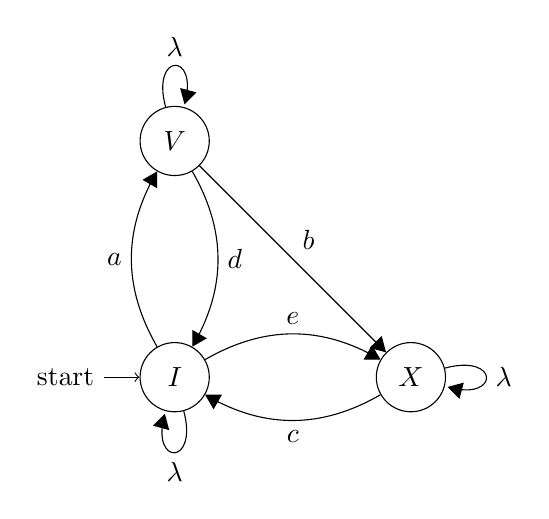
\begin{tikzpicture}
  [->,-triangle 60, node distance=3cm, auto, every loop/.append style={-triangle 60}]

  \node[initial,state] (I)              {$I$};
  \node[state]         (V) [above of=I] {$V$};
  \node[state]         (X) [right of=I] {$X$};

  \path (I) edge [bend left] node {$a$} (V)
            edge [bend left] node {$e$} (X)
        (V) edge [bend left] node {$d$} (I)
            edge             node {$b$} (X)
        (X) edge [bend left] node {$c$} (I);

  \path (I) edge [loop below] node {$\lambda$} ();
  \path (V) edge [loop above] node {$\lambda$} ();
  \path (X) edge [loop right] node {$\lambda$} ();

\end{tikzpicture}
\endgroup
%}%
\caption{State transition diagram for the state component of the dynamic transaction state.
  $I$ represents $\mathit{Idle}$, $V$ represents $\mathit{Eval}$, and $X$ represents $\mathit{Exec}$.
  \label{dt_state}}
\end{figure}

The dynamic transaction state $s_u(t)$ is itself a state transition system and much of the challenge in designing a scheduler revolves around the details of enforcing this transition system for concurrently executing transactions.
Figure~\ref{dt_state} shows the state transition diagram for the state component of the dynamic transaction state ($q$ of $s_u(t)$).
Each state has a self loop that allows a transaction to stay in the same state while another transaction changes state (indicated by $\lambda$).
There are two main paths through the transition system.
The path $abc$ corresponds to evaluating the precondition and immediately executing the immutable and mutable phases.
The path $adec$, for example, corresponds to evaluating the precondition and later executing the immutable and mutable phases.
Let $\Gamma$ be the set of transitions indicated in Figure~\ref{dt_state}.
Each element $\gamma \in \Gamma$ is a pair in $Q \times Q$.
The following condition states that every transition in a scheduler must obey the transition system described in Figure~\ref{dt_state}:
\begin{equation}
  \forall t, u : (s_u(t).q, s_u(t+1).q) \in \Gamma
\end{equation}
The precondition of a transaction is established as true or false as a result of leaving the $\mathit{Eval}$ state (transitions $b$ and $d$ in figure~\ref{dt_state}):
\begin{equation}
  \label{pre_establish}
  \forall t, u, s_u(t).q = \mathit{Eval} \land s_u(t+1).q \neq \mathit{Eval} : s_u(t+1).p \in \{0,1\}
\end{equation}
The precondition of a transaction must be true while executing the immutable and mutable phases:
\begin{equation}
  \label{pre_true}
  \forall t, u : s_u(t).q = \mathit{Exec} \implies s_u(t).p = 1
\end{equation}

A transaction that mutates the state of one or more components invalidates the precondition of all transactions whose preconditions are derived from the same state.
Let $\mathit{pre}: T \to H$ be a function that maps a transaction to the set of access pairs corresponding to the precondition of a transaction.
Let $\mathit{imm}(u)$ and $\mathit{mut}(u)$ be similarly defined functions that return the immutable phase access set and mutable phase access set for transaction $u \in T$.
All of these functions may be computed as part of composition analysis.
The set of transactions that are potentially affected by a given transaction $u \in T$ is given by the following function:
\begin{equation}
  \label{affected}
  \mathit{affected}(u) = { v \in T : \mathit{race}(\mathit{mut}(u), \mathit{pre}(v)) }
\end{equation}
The result of a transaction being executed has the effect of invalidating the precondition for all affected transactions:
\begin{multline}
  \forall t, u : s_u(t).q = \mathit{Exec} \land s_u(t+1).q \neq \mathit{Exec} \implies \\ \forall v \in \mathit{affected}(u) : s_v(t+1).p = \bot
\end{multline}
The previous requirement represents a worst case scenario where the transaction mutates all components in the mutable access set.
An obvious optimization is to only invalidate preconditions derived from the subset of instances that actually changed state.

A scheduler is safe if it avoids data races among the set of active transactions.
We define the dynamic access set of a transaction as follows:
\begin{equation}
  \label{access}
  \mathit{access}(s_u) = \begin{cases}
    \emptyset & \text{if $s_u.q = \mathit{Idle}$} \\
    \mathit{pre}(u) & \text{if $s_u.q = \mathit{Eval}$} \\
    \mathit{imm}(u) \cup \mathit{mut}(u) & \text{if $s_u.q = \mathit{Exec}$}
    \end{cases}
\end{equation}
A scheduler state is safe if there are no data races:
\begin{equation}
  \mathit{safe}(s) = \forall u, v \in T, u \neq v : \lnot \mathit{race} (\mathit{access}(s_u), \mathit{access}(s_v))
\end{equation}
A scheduler is safe if it only enters safe states:
\begin{equation}
  \label{race}
  \forall t : \mathit{safe}(s(t))
\end{equation}

%% The safety requirement expressed in Equation~\ref{race} influences every voluntary scheduling decision.
%% Consider the set of possible next states for a scheduler.
%% The transitions in figure~\ref{dt_state} can be classified into two groups.
%% Transitions $a$, $b$, and $e$ are voluntary and result in non-empty access sets while $d$ and $c$ are involuntary and result in empty access sets (Equation~\ref{access}).
%% Thus, we limit the discussion to scheduling steps where the scheduler is making a voluntary transition.
%% Let $\mathit{vol}(t) \subseteq T$ represent the subset of transactions that are candidates for a voluntary transition at time $t$ and let $\mathit{next}(u)$ represent the next transition state according to the system of figure~\ref{dt_state}.
%% Also, let $s(t) \downarrow u$ represent the result of substituting transaction state $u$ into $s(t)$.
%% A set of possible next states is given by:
%% \begin{equation}
%%   \mathit{candidates}(t) = \bigcup_{u \in \mathit{vol}(t)} s(t) \downarrow \mathit{next}(u)
%% \end{equation}
%% However, not every state in $\mathit{next}(t)$ is a valid state due to Equation~\ref{race}.
%% A refined set of next states is then:
%% \begin{equation}
%%   \mathit{next}(t) = \{ s \in candidates(t) : safe(s) \}
%% \end{equation}

In a fair scheduler, an enabled transaction cannot be postponed indefinitely.
Argument by contradiction is one approach to demonstrating that a scheduling algorithm is fair.
If one assumes that a scheduler is not fair, then there must be some scheduler state $s(t_c)$ that contains a transaction $u$ that is enabled in every subsequent state but never executed.
The ``enabledness'' described in the previous sentence is not the value $p$ in the definition of $s_u(t)$ which is the value known by the scheduler.
Rather, it refers to the actual value of the precondition based on the state contained in the component instance.
The argument is completed by demonstrating that the scheduler does in fact execute $u$.
For example, a scheduler that processes transactions in first-in first-out (FIFO) order eventually executes every transaction in the queue.

A scheduler design must reconcile the forces arising from the basic execution model, fairness, safety, and efficiency.
The basic execution model forces the scheduler to establish preconditions (Equation~\ref{pre_establish}) before executing the immutable and mutable phases (Equation~\ref{pre_true}).
Fairness compels the scheduler to execute certain transactions while safety compels the scheduler to avoid executing certain transactions (Equation~\ref{race}).
With respect to efficiency, a scheduler design may attempt to exploit the concurrency available in the set of transactions through parallel execution.

To illustrate the interplay among these forces, consider a concurrent and work-conserving scheduler.
Let the system consist of the set of transactions $S \cup \{ \tau \}$ where $S$ is a set of transactions that are safe with respect to each other and $\tau$ is a transaction that is not safe with respect to all transactions in $S$.
Thus, at any given time, the scheduler can be executing transactions in $S$ or $\tau$.
Suppose the scheduler is concurrently executing two transactions from $S$.
When one of the transactions terminates, the scheduler must immediately execute another transaction since it is work conserving.
For safety, the scheduler will execute another transaction from $S$ as it is unsafe to execute $\tau$.
This pattern of behavior induced by the work conserving nature of the scheduler may perpetually deny service to $\tau$.
For fairness, the scheduler must refrain from executing another transaction so that the $\tau$ transaction can be serviced.
Thus, with respect to parallel and concurrent execution, a scheduler design must balance gains in performance from exploiting parallelism with the requirement of fairness.

The scheduling problem for reactive components, then, is:  given a set of active transactions, select the next transaction for evaluation (precondition) or execution (immutable and mutable phase) subject to fairness and safety.

\section{Scheduler Classes}

Different factors may influence the design of transaction schedulers, which we distinguish according to four dimensions.
A given scheduler may be:  \emph{lazy} or \emph{eager}, \emph{oblivious} or \emph{knowledgeable}, \emph{cautious} or \emph{speculative}, and \emph{non-preemptive} or \emph{preemptive}.

\paragraph{Lazy and eager schedulers.}
A scheduler may be \emph{lazy} or \emph{eager} with respect to evaluating preconditions.
A lazy scheduler defers evaluating the precondition until the transaction is selected for execution (path $abc$ in Figure~\ref{dt_state}).
An eager scheduler evaluates preconditions after the state upon which they are based changes (path $ad$ in Figure~\ref{dt_state}).
The perceived benefit of a lazy scheduler is that it may reduce overhead by not evaluating preconditions while the perceived benefit of an eager scheduler is that it may only select actions which are enabled, which may result in more efficient use of acquired resources.

\paragraph{Oblivious and knowledgeable schedulers.}
We have considered two kinds of schedulers with respect to safety.
The first is an \emph{oblivious} scheduler that doesn't have direct access to the (global) scheduler state and therefore can't know the set of next states.
An oblivious scheduler selects a transaction and then determines if the transaction is safe to execute.
This typically involves a locking mechanism to ensure that all of the instances in the requisite access sets are available.
The second kind of scheduler is a \emph{knowledgeable} scheduler that does know the global scheduler state.
A knowledgeable scheduler can be proactive and maintain a set of transactions that are safe with respect to the set of active transactions.
This would allow a knowledgeable scheduler to efficiently select a safe action.
The open question is whether or not the efficiency of selection overcomes the overhead of maintaining the set of safe transactions.

\paragraph{Cautious and speculative schedulers.}
A \emph{cautious} scheduler avoids all race conditions and always satisfies the safety requirement of Equation~\ref{race}.
A \emph{speculative} scheduler optimistically evaluates preconditions and executes transactions but aborts them if a conflict is discovered.
Transactional memory is one technology that could be used to build a speculative scheduler.
For this work, we will assume that preconditions, immutable phases, and mutable phases are not aborted and leave the application of transactional memory to reactive components as future work.

\paragraph{Non-preemptive and preemptive schedulers.}
An \emph{active} transaction is one whose precondition is being evaluated or whose immutable or mutable phase is being executed.
An active transaction need not physically occupy a processor core.
This condition occurs in \emph{preemptive} schedulers that can interrupt a precondition, immutable phase, or mutable phase to do other work.
In contrast, a \emph{non-preemptive} scheduler does not interrupt the execution of a transaction, i.e., transactions are physically atomic.
Preemption may be useful to reduce the latency of transactions, support real-time priorities, etc.
We leave the application of preemption to reactive component schedulers as future work.

\section{Scheduler Design}

The previous sub-section illustrated a number of design dimensions for reactive component schedulers:  lazy vs. eager, oblivious vs. knowledgeable, cautious vs. speculative, and non-preemptive vs. preemptive.
For tractability, we will focus on the design and implementation of particular schedulers that are lazy, oblivious, cautious, and non-preemptive, and leave a more complete exploration of the design space for future work.
The goal of the following discussion is to introduce some of the issues when designing and implementing a scheduler, through a series of increasingly complex scheduler designs.
We will describe the concurrent schedulers in terms of \emph{threads}, which may be dedicated to physical processor cores or scheduled on one or more cores by an operating system.

%% \paragraph{Scheduler criteria.}
%% A scheduler is \emph{fair} if it meets the fairness criteria set forth in Chapter~\ref{model}.
%% A scheduler is \emph{safe} if it avoids conditions where one transaction is changing the state of the component while another transaction is reading or writing the same state.
%% A scheduler is \emph{responsible} if it only terminates when the precondition for every action is false.
%% Obviously, we are interested in fair, safe, and responsible schedulers as these schedulers enforce the semantics of reactive components.
%% The final criteria for a scheduler is efficiency which typically refers to either the computational complexity or storage complexity associated with its operation.
%% % Of primary interest is the \emph{selection efficiency} or the amount of computation required for the scheduler to determine the next action to execute.

\paragraph{Serial round-robin scheduler.}
Perhaps the simplest scheduler that can be implemented is a serial round-robin scheduler.
This design may be appropriate in the context of uniprocessor embedded systems with tight resource constraints.
The scheduler repeatedly cycles through the list of transactions, evaluating the precondition of each transaction and executing the immutable and mutable phases if the precondition was true.
If no transaction is executed in a cycle, then the scheduler terminates.
This scheduling algorithm is fair by virtue of the strict round-robin policy, safe from the fact that it is serial and non-preemptive, and responsible by definition.
The \emph{selection efficiency} of a scheduler is the number of transactions that must be selected before executing an enabled transaction or terminating.
The selection efficiency of this algorithm is $O(|T|)$ as illustrated by a system where one transaction that is perpetually enabled while all of the other transactions are perpetually disabled.

\paragraph{Serial scheduler with a transaction work queue.}
The perceived weakness of the serial round-robin scheduler is the overhead of evaluating preconditions that evaluate to false.
So, instead of cycling through the list of transactions, this scheduler maintains a work queue of transactions whose preconditions are true.
At initialization time, the scheduler populates the queue by evaluating the precondition of each transaction in the system.
The scheduler then repeatedly takes a transaction from the queue, executes it, and then inserts any newly enabled transactions, making this scheduler an eager scheduler.
To find newly enabled transactions, the scheduler uses the access set generated during composition analysis.
That is, after executing a transaction, the scheduler tests all of the transactions for the components in the access set and adds them to the queue if necessary.
Alternatively, the scheduler may assume that the precondition is true and insert the transaction, knowing that the precondition will be re-evaluated when the transaction is selected.
The scheduler terminates when the work queue is empty.
This scheduling algorithm is fair if the work queue is processed in first-in first-out (FIFO) order, safe because the algorithm is serial and non-preemptive, and responsible since an empty work queue implies no transaction is enabled.

The pathological scenario for the serial round-robin scheduler applies to this scheduler as well, so the worst-case selection efficiency of the algorithm is $O(|T|)$.
Assume that the most complex transaction in the system involves $c$ components and some component has a system-wide maximum transaction count of $a$.
In the worst case, the scheduler must evaluate $c \times a$ preconditions for every transaction that it executes.
Thus, the overhead associated with this scheduler is related to the compositional structure of the system that it is executing.
This overhead may be acceptable for systems where $c$ and $a$ are small or for systems whose average work queue size is small compared to the total number of transactions in the system.
This suggests that the average number of enabled transactions compared to the total number of transactions may be a useful way to analyze reactive component systems and schedulers.
For example, the serial round-robin scheduler would be appropriate for a \emph{heavily enabled} system while the serial scheduler with a transaction work queue would be appropriate for a \emph{lightly enabled} system.

\paragraph{Serial scheduler with an instance work queue.}
This scheduling algorithm attempts to squeeze a little more performance from the single-threaded scheduler with a transaction work queue.
The significant difference is that after the scheduler executes a transaction, it places the component instances that might have changed state into the work queue.
The work queue is initialized with all of the components in the system.
When processing a component on the work queue, the scheduler cycles through all of the transactions for that particular component.
The potential increase in performance comes from deferring the evaluations of the preconditions until absolutely necessary, i.e., lazy scheduling.
The scenario on which this scheduler attempts to capitalize is when some components are rarely involved in transactions.
An instance is enabled if at least one of its transactions is enabled.
Thus, this scheduler is appropriate for systems that are lightly enabled from the instance perspective.

\paragraph{Concurrent global round-robin scheduler.}
This scheduler runs $P > 1$ copies of a round-robin scheduler in parallel.
To be safe, we must devise a protocol that allows the threads to avoid concurrently executing transactions that may mutate the same state.
Using the assumption that a component instance is a proxy for its state variables, the scheduler locks all instances in the access set before evaluating the precondition and executing the transaction.
Recall that composition analysis determines the set of components that are involved in a transaction and how they are accessed ($\mathit{Read}$ or $\mathit{Write}$).
The acquired lock corresponds to the access type, which allows multiple threads to be reading a component but only one thread to be writing.
The locks are acquired in a determined order to avoid deadlock (Havender's Principle).
The concurrent global round-robin scheduler is fair so long as the underlying locking mechanism is fair, i.e., there is no reader or writer starvation.
The algorithm is also responsible, as each thread proves to itself that there are no enabled transactions left in the system.

An important concern with this algorithm is the locking required to coordinate access to component instances.
One negative characteristic caused by the locking is that a thread may become idle while waiting for a lock.
Thus, we might look for alternatives that allow a thread to do other useful work while waiting for a lock.
Another goal might be to look for ways to coordinate access to component instances without using locks at all.
Some of these ideas are explored later in this chapter.

\paragraph{Concurrent partitioned round-robin scheduler.}
Rather than have each thread cycle through the entire list of transactions, the concurrent partitioned round-robin scheduler divides the list of transactions among the available threads.
Like the global version, this algorithm is fair if the underlying locking mechanism is fair.
Similarly, this algorithm is safe as locks are used to coordinate access to component state.
However, for this algorithm to be responsible, we must add a protocol that allows the threads to detect that the system has reached the termination condition.

The termination protocol consists of a barrier synchronization and then a check to establish the termination condition.
The termination protocol begins when a scheduler thread sends a termination request to the \emph{manager thread}.
To process a termination request, the manager thread stops each scheduler thread and then checks that all transactions are disabled.
If all of the transactions are disabled, the system terminates.
Otherwise, the manager thread restarts the scheduler threads.
A scheduler thread may choose to request termination at any time and different heuristics may be used to determine when a scheduler thread makes the termination request.
Deferring the request has the advantage of avoiding the termination protocol overhead.
For example, a scheduler thread might wait until it makes a complete pass through its list of transactions without executing one before making the request.

Such a centralized termination protocol is rather disruptive as it must stop the system to check for termination.
Thus, one goal may be to let a thread idle itself and be woken up by active neighbors.
Similarly, the scheduler threads can check for the termination condition in parallel and wake up all of their neighbors if a transaction is enabled.
Finally, the manager thread may be done away with entirely and the protocol rewritten as a distributed protocol, as we discuss below.

\section{Scheduler Implementations}

We now describe two specific scheduler designs that we chose for implementation and evaluation.
Each scheduler takes a different approach to the design dimensions described previously, resulting in distinct consequences for systems that use it.

\paragraph{Concurrent scheduler with a global instance work queue.}
The first scheduler that we implemented was a concurrent scheduler with a global instance work queue.
The work queue is initialized to contain all of the instances in the system.
The scheduler threads take an instance from the work queue, select and execute all transactions in the instance, and insert any instances that might have changed state back into the work queue.
Fairness is achieved by processing the queue in FIFO order and safety is achieved through the aforementioned locking scheme.
The termination protocol for this scheduler involves counting the number of instances that are currently in the queue and the number of instances currently being processed by the scheduler threads.
When this count drops to zero, there are no enabled instances in the system and the system may terminate responsibly.

One potential weakness of this scheduler is the synchronization required to coordinate access to the work queue, which adds a communication overhead and may create contention if the scheduler threads are lightly loaded, i.e., they frequently return to the queue looking for work.
Thus, the scalability of this scheduler is a concern.

\paragraph{Concurrent partitioned round-robin scheduler with asynchronous locking and distributed termination.}
One of the goals when designing this scheduler was to avoid the blocking behavior and overhead of locking observed during out evaluations of the concurrent scheduler with a global instance work queue.
The pthreads reader/writer locks used to protect each component instance were replaced by asynchronous reader/writer locks implemented in user-space.
The asynchronous locks consist of a spin lock, variables indicating the status of the lock, and a queue of requests.
To acquire a lock for a component, a scheduler thread first acquires the spin lock and then checks if the lock can be acquired immediately, which it can if either the lock has no owner or the thread is a reader (i.e., it is requesting a read lock); the lock has already been locked by another reader; and there are no writers in the queue.
Otherwise, the request is placed on the queue.
A scheduler thread failing to acquire the lock can either idle or attempt to execute a different transaction.
When a lock is unlocked, the thread at the front of the queue is notified so it may resume processing the transaction that it was attempting to execute.
The protocol avoids reader and writer starvation and ensures fairness since the queue is processed in FIFO order.
This scheduler is \emph{work conserving} since a scheduler thread continues to execute transactions instead of blocking.
However, scheduler threads do not steal work from other threads.

The aforementioned centralized termination protocol has the potential to be disruptive.
Thus, the motivation for a distributed termination protocol is to keep the scheduler threads as busy as possible meaning that the termination protocol is started infrequently and the termination protocol itself aborts as early as possible if the termination condition has not been reached.
For this scheduler, the threads are arranged in a ring and communicate using asynchronous message queues.
Messages are stamped with the id of the originating thread.
The protocol forwards messages around the ring so a thread receiving a message from itself knows that all of the threads have processed that message.

Like the centralized version, the ring-based distributed termination protocol consists of a synchronization phase and checking phase.
Scheduler threads begin in the RUN state where they are actively cycling through their lists of transactions.
When a scheduler thread determines that termination may be possible, it sends a message to its neighbor indicating that it is entering the SYNC state.
If the neighbor thread is in the RUN state, it resolves to send a reset message the next time it executes a transaction which means that the termination condition has not been established.
Otherwise, the neighbor thread itself is already in the SYNC state and forwards the message.
Reset messages are unconditionally forwarded around the ring and cause all threads to enter the RUN state.
Synchronization messages are only forwarded if the thread receiving the message is in the SYNC state.
Thus, if a thread receives its own synchronization message, all other threads in the scheduler are in the SYNC state.
Multiple threads may receive their own synchronization message at the same time.

The goal of the synchronization phase is to establish a common point of reference for determining if any transaction is enabled.
When a thread receives its own synchronization message, it sends a message to its neighbor that it is entering the CHECK state.
This message is forwarded around the ring causing all of the threads to enter the CHECK state.
The CHECK state is like the modified RUN state in that any executed transaction causes a reset message to circulate around the ring.
A thread that cycles through its list of transactions and finds no enabled transactions sends a wait message to its neighbor and enters the WAIT state.
If the neighbor is in the WAIT state, it forwards the message.
If a thread receives its own wait message, then all of the threads are in the WAIT state and the termination condition has been established.
Upon receiving its own wait message, a thread sends a termination message causing all threads to terminate.

\section{Scheduler Evaluation}

The utility of the reactive component model rests on the ability to execute reactive programs effectively.
The challenge, then, is to design and implement effective schedulers subject to the constraints and limitations imposed by the model.
The exercise of developing and evaluating schedulers may suggest possible improvements to the model or provide evidence that core features of the model resist efficient implementation.
The definition of an effective scheduler will vary by platform and problem domain.
For example, embedded systems may prefer a single-threaded scheduler with minimal memory requirements and power-awareness.
Our focus in this work is to make progress on general-purpose concurrent schedulers.
We propose the following metrics for the evaluation of a general-purpose scheduler:
\begin{description}
\item[Throughput:] the number of transactions executed per second.
Given the same system, a scheduler with higher throughput is preferable to a system with lower throughput as it is accomplishing more work per unit of time.
Throughput can also be defined for specific problems by defining a unit of work and measuring the number of work units processed per unit of time.
\item[Latency:] the amount of time between an transaction becoming enabled and being executed.
The goal in measuring the latency between a transaction becoming enabled and its execution is to quantify the responsiveness of the scheduler.
An interactive application may prefer a scheduler that executes enabled transactions promptly to aid in providing a good user experience or other benefit.
Like throughput, latency may also be defined for units of work.
\item[Utilization:] the fraction of the CPUs used.
Utilization is a measure of how efficiently the scheduler is using the CPUs and can be used to quantify an improvement in throughput or latency.
For example, a 10\% increase in throughput accompanied by a 10\% increase in utilization may be acceptable while a 10\% increase in throughput with a 100\% increase in utilization may not be acceptable.
\end{description}
Both throughput and latency may be considered for individual transactions, or may be aggregated over all transactions in the system.

\paragraph{Evaluation approach.}
We used two variants of the clock system from Chapter~\ref{model} to evaluate the two scheduler implementations.
The first variant is the fully-factored clock system augmented with counters that cause termination\footnote{https://github.com/jrw972/rc/blob/master/samples/clock3.rc}.
In this system, there are three components of interest:  the Client, the Server, and the Counter.
This system has three transactions:
\begin{itemize}
  \item Request - The client requests the time from the server.  This involves the Client and the Server.
  \item Response - The server responds with the time.  This involves the Client, the Server, and the Counter.
  \item Tick - The counter increments the current time.  This involves the Counter.
\end{itemize}
This system will be denoted as the \emph{AsyncClock} system.

\begin{figure}
\centering
\resizebox{.5\textwidth}{!}{%
\begingroup
\fontsize{10pt}{12pt}\selectfont
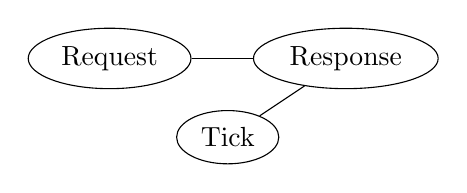
\begin{tikzpicture}

\node[draw, ellipse] (Request) at (0,0) {Request};
\node[draw, ellipse] (Response) at (3,0) {Response};
\node[draw, ellipse] (Tick) at (1.5,-1) {Tick};

\draw (Request) -- (Response);
\draw (Tick) -- (Response);

\end{tikzpicture}
\endgroup
}%
\caption{Race graph for the AsyncClock system.  Each node is a transaction.  Nodes sharing an edge cannot be executed concurrently due to potentially mutated shared state. \label{clock_system_mutex}}
\end{figure}

Figure~\ref{clock_system_mutex} shows a \emph{race graph} for the AsyncClock system.
Each node in the graph is a transaction $u \in T$.
Let $\mathit{acc}(u) = \mathit{pre}(u) \cup \mathit{imm}(u) \cup \mathit{mut}(u)$.
An edges exists between two nodes $u,v \in T$ if $\mathit{race}(\mathit{acc}(u), \mathit{acc}(v))$.
Nodes sharing an edge cannot be executed concurrently due to potentially mutated shared state.
Conversely, nodes that are not linked by an edge can be executed concurrently.
For the purpose of evaluating schedulers, the clock system has the important characteristic that Request and Tick can be executed concurrently while Response must be executed independently.
Another useful feature of this system is that each component has exactly one transaction, and thus, a  work queue of instances may also be viewed as a work queue of transactions.

The second variant is a simplified version of the clock system consisting of a Tick transaction that increments the counter and a Request transaction that uses a getter to sample the counter\footnote{https://github.com/jrw972/rc/blob/master/samples/clock4.rc}.
The counter creates a race between the two transactions so that they cannot be executed concurrently.
This system will be denoted as the \emph{SyncClock} system.

For comparison, we implemented threaded versions of the AsyncClock and SyncClock systems using the POSIX threads library (pthreads).
The AsyncClock implementation attempts to preserve the spirit of the AsyncClock system by being as asynchronous as possible.
This implementation uses three threads corresponding to the Request, Response, and Tick transactions.
The Request and Response threads share a flag variable that is protected by a mutex and condition variable, to implement the asynchronous request/response protocol.
The Response and Tick threads share a counter variable that is protected by a mutex.
The SyncClock implementation attempts to preserve the spirit of the SyncClock system.
In this design, there is one thread sampling the counter while another thread is incrementing the counter.
The two threads synchronize access to the counter through a single mutex.
For convenience, experiments involving a pthreads implementation will be labeled \emph{Thread}, experiments involving the concurrent scheduler with a global instance work queue will be labeled \emph{Instance}, and experiments involving the concurrent partitioned  round-robin scheduler with asynchronous locking and distributed termination will be labeled \emph{Partitioned}.

The AsyncClock and SyncClock systems were executed 1,000 times to profile the performance of each scheduler.
The programs are instrumented with profiling code that records the total execution time and timestamps for each transaction.
The timestamps are stored in memory and written after the scheduler terminates to avoid disruptions in timing due to output.
The Request and Tick transactions were limited to 10,000 executions.
Thus, each SyncClock run generates 20,000 data points.
In the AsyncClock system, the relationship between Request and Response causes Response to be executed 10,000 times as well.
Thus, each AsyncClock run generates 30,000 data points.
The throughput for a single run is determined by dividing the total number of transactions (20,000 or 30,000) by the total time used for execution.
The utilization was determined using the \verb+time+ utility and the number of context switches was determined using the \verb+getrusage+ system call before and after the execution of the system.
The latency for each transaction is determined by computing the difference between the transaction start time and the end time of the enabling transaction.
For the SyncClock system, this is $Request_{t+1} - Request_{t}$ and $Tick_{t+1} - Tick_{t}$.
For the AsyncClock system, this is $Request_{t+1} - Response_{t}$, $Response_{t+1} - Request_{t}$, and $Tick_{t+1} - Tick_{t}$.
For the SyncClock system, $1,000 \times 20,000 = 20,000,000$ latency points were collected.
For the AsyncClock system, $1,000 \times 30,000 = 30,000,000$ latency points were collected.

Placing all transactions in a run on a timeline according to their start times, we define the \emph{entanglement} of a run to be the number of adjacent transactions on the timeline that were executed in different threads.
The entanglement is used to measure the granularity of the concurrency between the scheduler threads.
Given that each run executes the same number of transactions, a high entanglement indicates ``fine'' concurrency, i.e., threads are executing transactions in parallel or execution is rapidly alternating between the threads, while a low entanglement indicates ``coarse'' concurrency.
Entanglement may be forced by the scheduler, or may occur opportunistically, or not at all.
The start time for threads influences entanglement as an operating system may execute a thread to completion before starting another thread.
The garbage collection actions are not included in the entanglement calculation to facilitate comparison with the pthread implementations.

\begin{table}
\center
\begin{tabular}{rl}
Machine Model:    & Lenovo G570 Laptop \\
Operating System: & Ubuntu 14.04 \\
Processor:        & Intel Pentium B960 2.20GHz \\
Architecture:     & 64-bit \\
Cores:            & 2 \\
Memory:           & 4GB \\
Kernel:           & 3.13.0-77-generic \#121-Ubuntu SMP \\
Compiler:         & g++ 4.8.4 \\
C library:        & glibc 2.19 \\
POSIX threads:    & glibc 2.19 \\
C++ library:      & glibc++ 3.4.19 \\
\end{tabular}
\caption{Experimental environment used for scheduler testing.\label{environment}}
\end{table}

Table~\ref{environment} describes the environment used to perform the scheduler experiments\footnote{The version of the code used for this evaluation bears the tag ``clock\_experiment2'' and can be found at https://github.com/jrw972/rc/releases/tag/clock\_experiment2.}.
The timestamp resolution reported by the operating system was 1 ns.
The Instance and Partitioned schedulers were configured to use two threads.
The Thread applications for the AsyncClock and SyncClock systems were designed to use three and two threads, respectively.
The raw data for the experiments can be obtained by emailing the author\footnote{jrw972@gmail.com}.

\begin{figure}[H]
\center
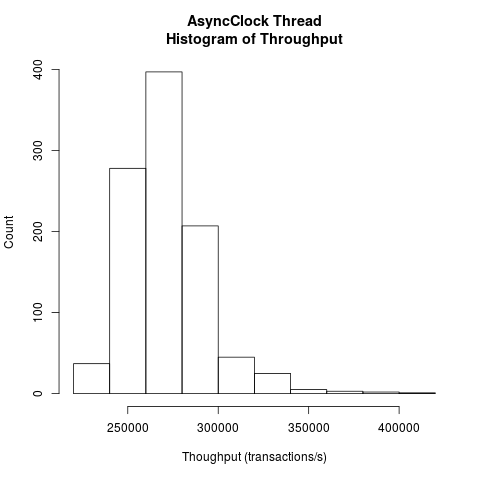
\includegraphics[height=.4\textheight]{async_thread_throughput_hist.png}
\caption{AsyncClock Thread Histogram of Throughput}
\label{async_thread_throughput}
\end{figure}

\begin{figure}[H]
\center
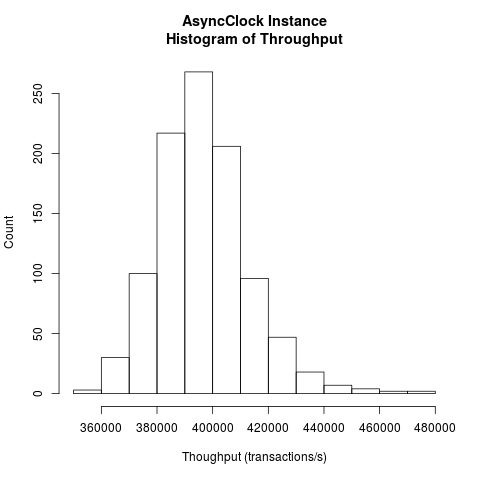
\includegraphics[height=.4\textheight]{async_instance_throughput_hist.png}
\caption{AsyncClock Instance Histogram of Throughput}
\label{async_instance_throughput}
\end{figure}

\begin{figure}[H]
\center
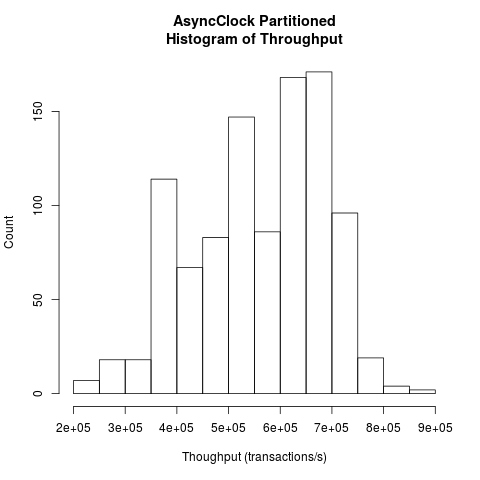
\includegraphics[height=.4\textheight]{async_partitioned_throughput_hist.png}
\caption{AsyncClock Partitioned Histogram of Throughput\label{async_partitioned_throughput}}
\end{figure}

\paragraph{AsyncClock results.}
Figures~\ref{async_thread_throughput}, \ref{async_instance_throughput}, and \ref{async_partitioned_throughput} show histograms of the throughput for the Thread, Instance, and Partitioned experiments, respectively.
The throughput for the Thread and Instance experiments appear to have ``regular'' distributions while the throughput for Partitioned is ``irregular.''
Transactions are randomly and statically allocated to execution threads in the Partitioned scheduler.
In the AsyncClock system, there are seven transactions where three correspond to Request, Response, and Tick, and the other four correspond to garbage collection actions for Client, Server, Counter, and System components.
Thus, there are $2^7 = 128$ mappings of transactions to execution threads.
Given the symmetry of threads, this results in 64 possible arrangements which are shown in Appendix~\ref{partition_tables} in Table~\ref{async_partitions}.
Some of these arrangements will place all transactions in one thread, leading to improved or degraded performance, e.g., `A'.
Some arrangements will place Request and Tick in different threads, allowing the potential concurrency among these actions to be exploited, e.g., `B'.
Some arrangements will place the Tick transaction and garbage collection action for Counter on different threads, creating lock contention, e.g., `C'.
Thus, the throughput for the Partitioned scheduler is a mixture of distributions corresponding to the different partitioning schemes.

\begin{figure}[H]
\center
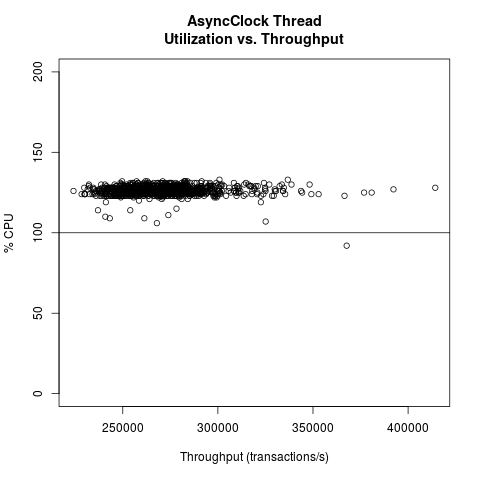
\includegraphics[height=.4\textheight]{async_thread_throughput_utilization.png}
\caption{AsyncClock Thread Utilization vs. Throughput}
\label{async_thread_throughput_utilization}
\end{figure}

\begin{figure}[H]
\center
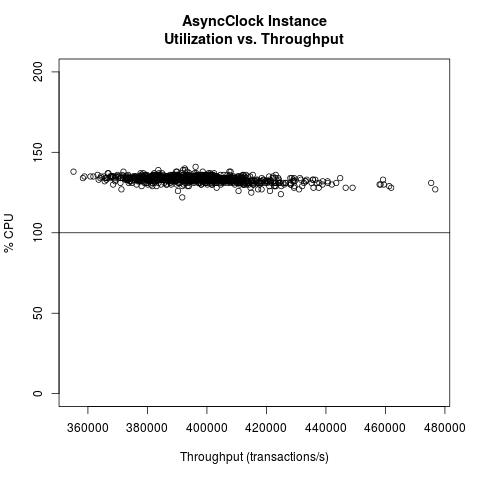
\includegraphics[height=.4\textheight]{async_instance_throughput_utilization.png}
\caption{AsyncClock Instance Utilization vs. Throughput}
\label{async_instance_throughput_utilization}
\end{figure}

\begin{figure}[H]
\center
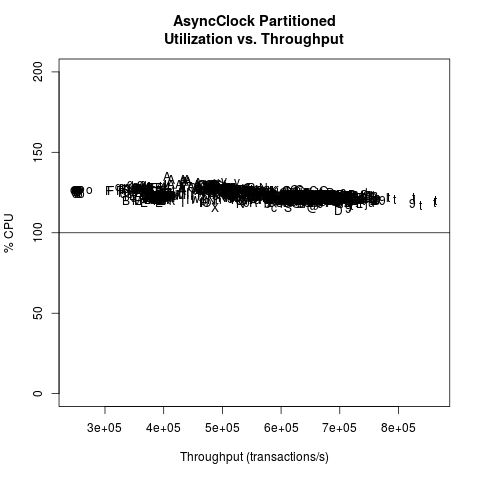
\includegraphics[height=.4\textheight]{async_partitioned_throughput_utilization.png}
\caption{AsyncClock Partitioned Utilization vs. Throughput}
\label{async_partitioned_throughput_utilization}
\end{figure}

Figures~\ref{async_thread_throughput_utilization}, \ref{async_instance_throughput_utilization}, and \ref{async_partitioned_throughput_utilization} show plots of utilization versus throughput for the Thread, Instance, and Partitioned experiments, respectively.
Most of the runs achieve a utilization greater than 100\%.
For the Instance and Partitioned schedulers, there appears to be slight trend where utilization decreases with increased throughput.
This is most likely the result of locking behavior where runs that (randomly) experience better locking behavior simultaneously achieve higher throughput and lower utilization due to less locking overhead.

\begin{figure}[H]
\center
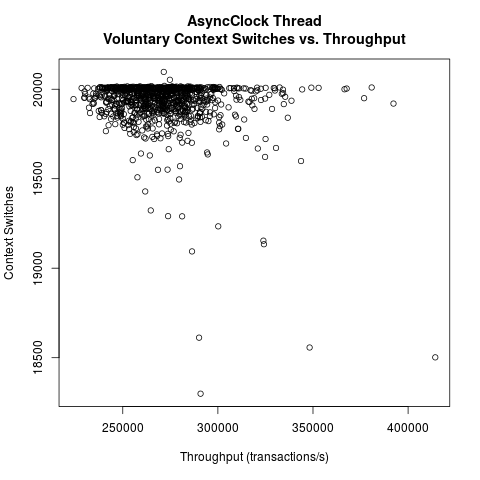
\includegraphics[height=.4\textheight]{async_thread_throughput_context.png}
\caption{AsyncClock Thread Voluntary Context Switches vs. Throughput}
\label{async_thread_throughput_context}
\end{figure}

\begin{figure}[H]
\center
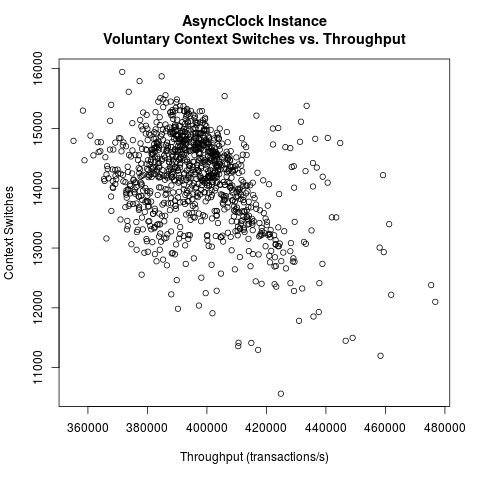
\includegraphics[height=.4\textheight]{async_instance_throughput_context.png}
\caption{AsyncClock Instance Voluntary Context Switches vs. Throughput}
\label{async_instance_throughput_context}
\end{figure}

\begin{figure}[H]
\center
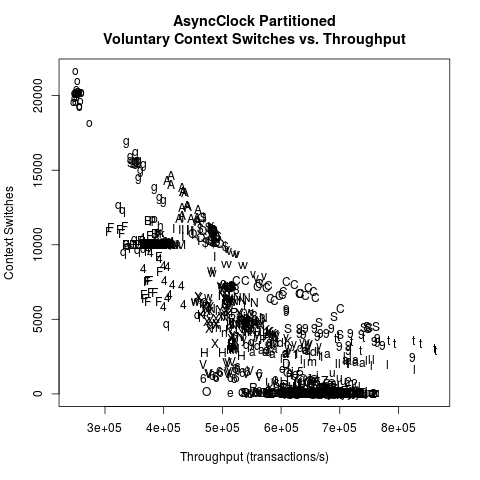
\includegraphics[height=.4\textheight]{async_partitioned_throughput_context.png}
\caption{AsyncClock Partitioned Voluntary Context Switches vs. Throughput}
\label{async_partitioned_throughput_context}
\end{figure}

Figures~\ref{async_thread_throughput_context}, \ref{async_instance_throughput_context}, and \ref{async_partitioned_throughput_context} show plots of voluntary context switches versus throughput for the Thread, Instance, and Partitioned experiments, respectively.
Voluntary context switches include the situation where a thread blocks while waiting for a lock and is swapped out.
The Thread scheduler appears to have a consistently high number of context switches.
This is expected since there are three threads competing for two processors.
The Instance scheduler has fewer context switches and perhaps shows a slight trend where throughput increases with fewer context switches.
As previously stated, this is most likely the result of locking behavior.
The Partitioned scheduler shows a strong trend of throughput increasing with fewer context switches.
Furthermore, the partitions appear to cluster together.
For example, all of the runs for partition `o' of Table~\ref{async_partitions} appear in the upper left of Figure~\ref{async_partitioned_throughput_context}, while the runs for partition `t' appear in the lower right.
In partition `o', thread 0 contains System, Counter, Tick, Request, and Response while thread 1 contains Server and Client.
This mapping serializes the execution (Request, Response, and Tick are on one thread) and is subject to contention arising from the Server and Client garbage collection actions competing with Request and Response.
In partition `t', thread 0 contains System, Counter and Tick while thread 1 contains Server, Client, Response, and Request.
The only contention in this mapping is between Response in thread 1 and Counter and Tick in thread 0.

\begin{figure}[H]
\center
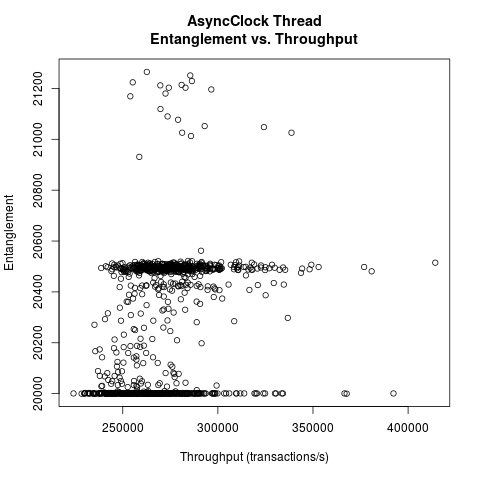
\includegraphics[height=.4\textheight]{async_thread_throughput_entanglement.png}
\caption{AsyncClock Thread Entanglement vs. Throughput}
\label{async_thread_throughput_entanglement}
\end{figure}

Figure~\ref{async_thread_throughput_entanglement} shows a plot of entanglement versus throughput for the Thread experiment.
The Thread scheduler has a minimum entanglement of 20,000, which is caused by the forced interleaving of the Request and Response threads, and a maximum entanglement of 30,000.
Thus, the lowest band in Figure ~\ref{async_thread_throughput_entanglement} corresponds to no entanglement with the Tick thread.
In these cases, the Linux thread scheduler executes the Request/Response threads first and the Tick thread second (or vice versa).
The generally low entanglement shows that the Linux scheduler prefers to serialize the execution.
This is reasonable given that the Thread scheduler is subject to a performance hit caused by context switches as previously described.
The upper band suggests a bound on the allowed entanglement.
One explanation for this behavior is that the Linux scheduler may limit context switches, which has the effect of limiting the entanglement in the Thread scheduler.
Another explanation is that the entanglement may be limited based on the threads starting at different times.

\begin{figure}[H]
\center
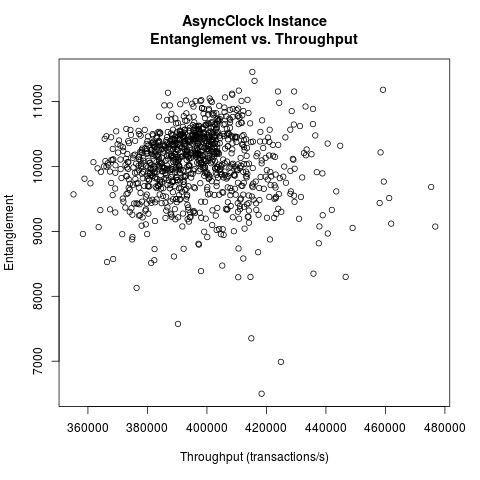
\includegraphics[height=.4\textheight]{async_instance_throughput_entanglement.png}
\caption{AsyncClock Instance Entanglement vs. Throughput}
\label{async_instance_throughput_entanglement}
\end{figure}

Figure~\ref{async_instance_throughput_entanglement} shows a plot of entanglement versus throughput for the Instance experiment.
The minimum entanglement is 0 and the maximum entanglement is 30,000\footnote{Let Transaction(Thread) indicate that the transaction was executed by the corresponding thread.  The following pattern when repeated 5,000 times generates an entanglement of 30,000:  Request(0) Tick(1) Response(0) Request(1) Tick (0) Response (1).}.
This plot does not appear to show a strong relationship between throughput and entanglement.

\begin{figure}[H]
\center
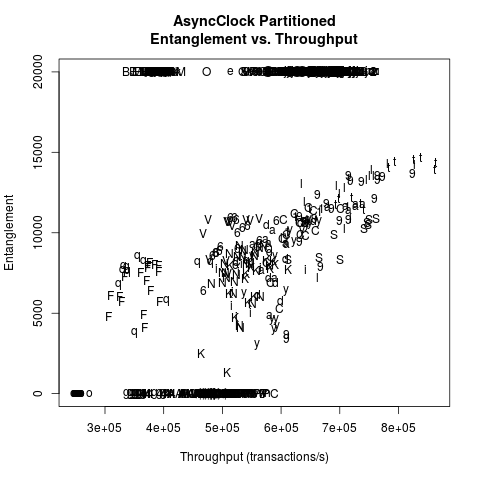
\includegraphics[height=.4\textheight]{async_partitioned_throughput_entanglement.png}
\caption{AsyncClock Partitioned Entanglement vs. Throughput}
\label{async_partitioned_throughput_entanglement}
\end{figure}

Figure~\ref{async_partitioned_throughput_entanglement} shows a plot of entanglement versus throughput for the Partitioned experiment.
This plot has a band at 20,000 that contains roughly half of the samples (513/1000).
These correspond to arrangements where Request and Response are mapped to different execution threads which forces an entanglement of 20,000.
Half of the remaining samples have no entanglement (246/1000).
These correspond to arrangements where the Request, Response, and Tick transactions are mapped to the same execution thread where no entanglement is possible.
The remaining quarter of the samples (241/1000) correspond to arrangements where Request and Response are in one execution thread while Tick is in the other.
These show varying degrees of entanglement with perhaps a slight trend toward increasing throughput with greater entanglement.
This is expected because the concurrency between Request and Tick can be exploited in these arrangements.

\begin{figure}[H]
\center
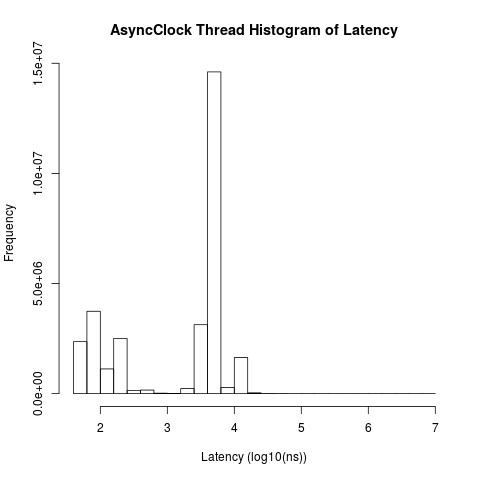
\includegraphics[height=.4\textheight]{async_thread_latency_hist.png}
\caption{AsyncClock Thread Histogram of Latency}
\label{async_thread_latency}
\end{figure}

\begin{figure}[H]
\center
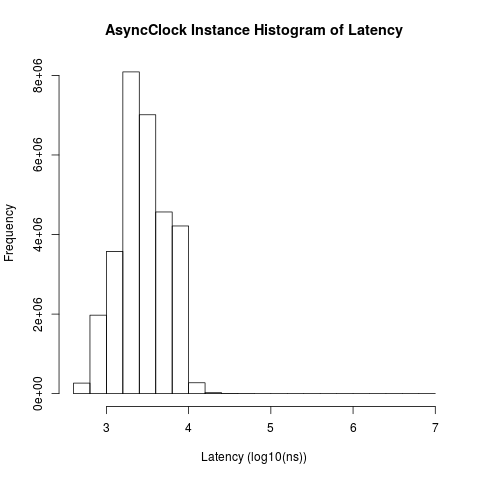
\includegraphics[height=.4\textheight]{async_instance_latency_hist.png}
\caption{AsyncClock Instance Histogram of Latency}
\label{async_instance_latency}
\end{figure}

\begin{figure}[H]
\center
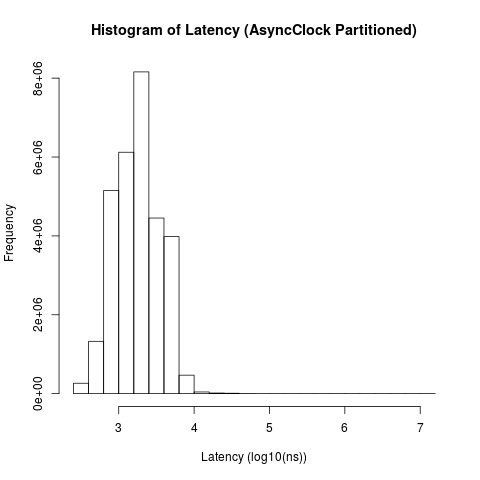
\includegraphics[height=.4\textheight]{async_partitioned_latency_hist.png}
\caption{AsyncClock Partitioned Histogram of Latency}
\label{async_partitioned_latency}
\end{figure}

Figures~\ref{async_thread_latency}, \ref{async_instance_latency}, and \ref{async_partitioned_latency} show histograms of the latency for the Thread, Instance, and Partitioned experiments, respectively.
All plots of latency use a logarithmic x-axis, as the latency distributions have very long tails.
For Thread, the mean latency of the transactions are as follows:
\begin{center}
\begin{tabular}{cr}
Tick     & 0.11769us \\
Request  & 5.30299us \\
Response & 5.63980us \\
\end{tabular}
\end{center}
Thus, the distribution on the left in Figure~\ref{async_thread_latency} corresponds to the latency of the Tick transaction while the distribution on the right corresponds to the latency of Request and Response.
In the Thread scheduler, Tick transactions can be executed in quick succession as they are in a tight loop.
For the Instance scheduler, the mean latency of the transactions are as follows:
\begin{center}
\begin{tabular}{cr}
Tick     & 5.22393us \\
Request  & 2.83083us \\
Response & 2.58799us \\
\end{tabular}
\end{center}
The Instance scheduler tends to serialize the execution of transactions for AsyncClock to avoid race conditions.
Thus, Tick has roughly twice the latency of Request and Response since Tick is always enabled while Request and Response are enabled by each other.
For Partitioned, the mean latency of the transactions are as follows:
\begin{center}
\begin{tabular}{cr}
Tick     & 2.49278us \\
Request  & 2.31450us \\
Response & 2.06478us \\
\end{tabular}
\end{center}
The work-conserving nature of the Partitioned scheduler allows it to achieve a lower average latency for all transactions when compared to the Instance scheduler.

\begin{figure}[H]
\center
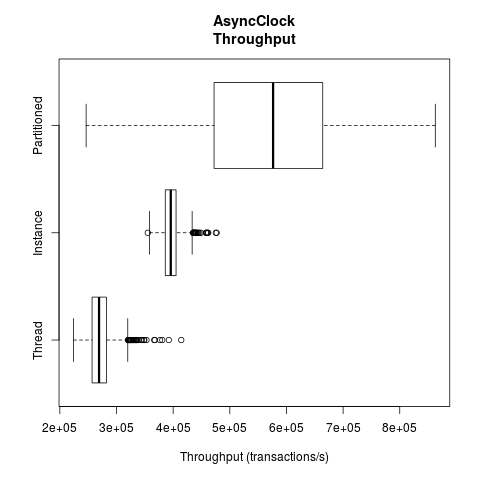
\includegraphics[height=.4\textheight]{async_throughput_box.png}
\caption{AsyncClock Throughput}
\label{async_throughput_box}
\end{figure}

Figure~\ref{async_throughput_box} shows a box plot of the throughput for the Thread, Instance, and Partitioned experiments.
The quantiles of the throughput in transactions/s for each scheduler are as follows:
\begin{center}
\begin{tabular}{crrrrr}
Scheduler   &       0\%   &    25\%     &    50\%     &    75\%     &   100\% \\
\hline
Partitioned &   246,370.0 &   472,679.2 &   576,411.0 &   664,042.5 &    862,717.0 \\
Instance    &   355,158.0 &   386,067.8 &   395,796.0 &   405,083.8 &    476,759.0 \\
Thread      &   224,107.0 &   256,876.0 &   269,193.5 &   282,329.0 &    414,293.0 \\
\end{tabular}
\end{center}
The work-conserving nature of the Partitioned scheduler allows it to achieve a higher throughput than the Instance scheduler, and its ability to avoid context switches allows it to achieve a higher throughput than the Thread scheduler.
However, the results also demonstrate the variability in the throughput due to the many modes of partitioning.
Thus, the Partitioned scheduler could be improved by using the race graph to avoid ``bad'' partitions.

\begin{figure}[H]
\center
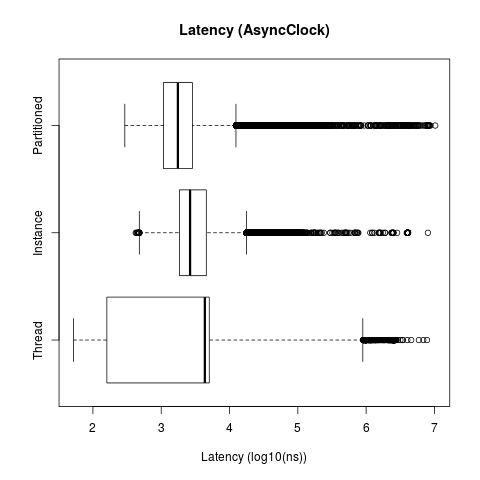
\includegraphics[height=.4\textheight]{async_latency_box.png}
\caption{AsyncClock Latency}
\label{async_latency_box}
\end{figure}

Figure~\ref{async_latency_box} shows a box plot of the latency for the Thread, Instance, and Partitioned experiments.
The quantiles of the latency (in ns) for each scheduler are as follows:
\begin{center}
\begin{tabular}{crrrrr}
Scheduler &       0\%  &    25\%  &    50\%  &    75\%  &   100\% \\
\hline
Partitioned & 293 & 1,075 & 1,754 & 2,861 & 10,296,400 \\
Instance    & 423 & 1,851 & 2,645 & 4,569 &  8,028,100 \\
Thread      &  52 &   160 & 4,352 & 5,051 &  7,791,400 \\
\end{tabular}
\end{center}
The Thread scheduler achieves the lowest latency via the Tick transaction due to its work-conserving nature and optimized locking scheme.

Both the Instance and Partitioned schedulers contain transactions for performing garbage collection.
These transactions do not actually perform any work since none of the transactions in the AsyncClock system allocate memory.
The Instance scheduler executed an average of 33,053 garbage collection actions per run while the Partitioned scheduler executed an average of 97,078 garbage collection actions per run.
The excessive number of collections performed by the Partitioned scheduler shows a potential problem between the garbage-collection-as-an-action idea and work conserving schedulers, as a work conserving scheduler can always find more work to do in garbage collection attempts.
Ideally, a scheduler would be designed to not even select a garbage collection action until it has a high probability of actually collecting garbage.

\clearpage

\begin{figure}[H]
\center
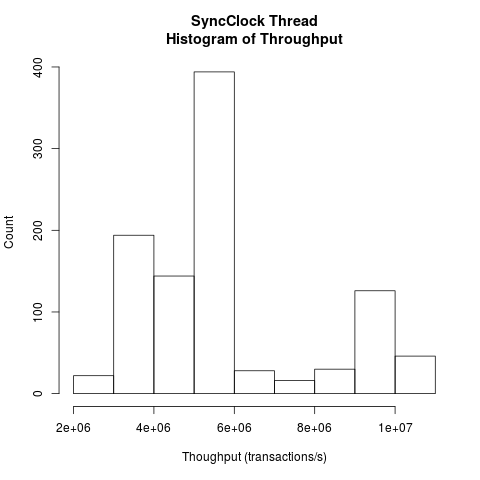
\includegraphics[height=.4\textheight]{sync_thread_throughput_hist.png}
\caption{SyncClock Thread Histogram of Throughput}
\label{sync_thread_throughput}
\end{figure}

\begin{figure}[H]
\center
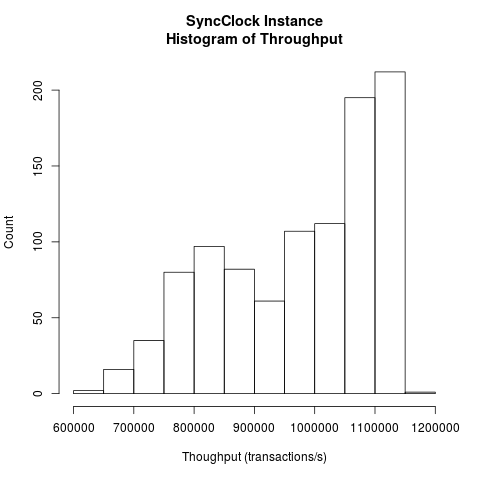
\includegraphics[height=.4\textheight]{sync_instance_throughput_hist.png}
\caption{SyncClock Instance Histogram of Throughput}
\label{sync_instance_throughput}
\end{figure}

\begin{figure}[H]
\center
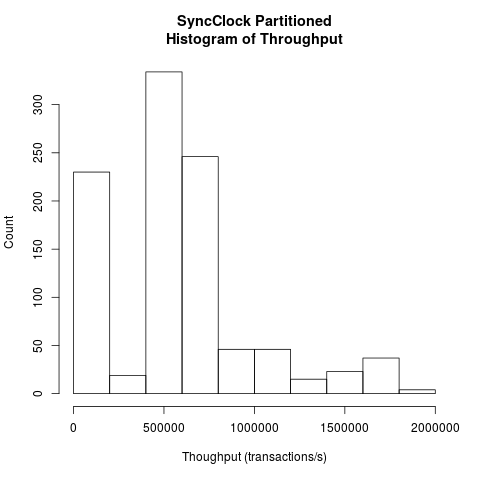
\includegraphics[height=.4\textheight]{sync_partitioned_throughput_hist.png}
\caption{SyncClock Partitioned Histogram of Throughput}
\label{sync_partitioned_throughput}
\end{figure}

\paragraph{SyncClock results.}
Figures~\ref{sync_thread_throughput}, \ref{sync_instance_throughput}, and \ref{sync_partitioned_throughput} show histograms of the throughput for Thread, Instance, and Partitioned experiments, respectively.
The throughput curves of the Thread and Instance experiments appear to be combinations of two or three distributions.
As in the AsyncClock experiments, the throughput for the Partitioned scheduler is a mixture of distributions arising from different partitioning schemes.
In the SyncClock system, there are two components and two transactions resulting in 8 possible partitions.
The list of partitions is given in Appendix~\ref{partition_tables} in Table~\ref{sync_partitions}.

\begin{figure}[H]
\center
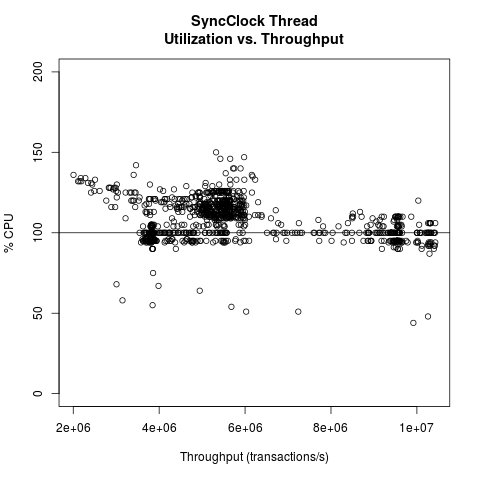
\includegraphics[height=.4\textheight]{sync_thread_throughput_utilization.png}
\caption{SyncClock Thread Utilization vs. Throughput}
\label{sync_thread_throughput_utilization}
\end{figure}

\begin{figure}[H]
\center
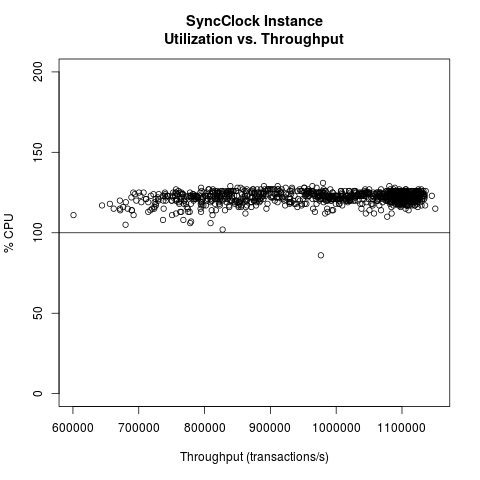
\includegraphics[height=.4\textheight]{sync_instance_throughput_utilization.png}
\caption{SyncClock Instance Utilization vs. Throughput}
\label{sync_instance_throughput_utilization}
\end{figure}

\begin{figure}[H]
\center
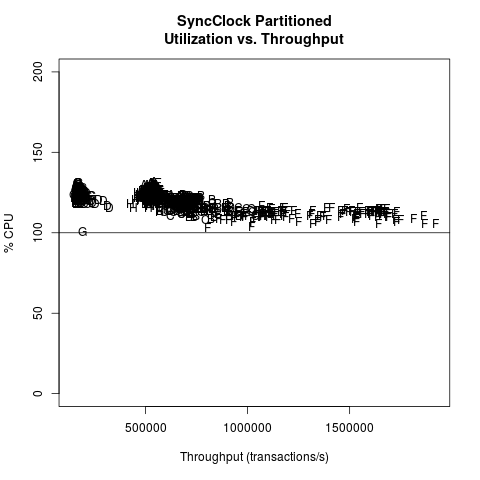
\includegraphics[height=.4\textheight]{sync_partitioned_throughput_utilization.png}
\caption{SyncClock Partitioned Utilization vs. Throughput}
\label{sync_partitioned_throughput_utilization}
\end{figure}

Figures~\ref{sync_thread_throughput_utilization}, \ref{sync_instance_throughput_utilization}, and \ref{sync_partitioned_throughput_utilization} show plots of utilization versus throughput for the Thread, Instance, and Partitioned experiments, respectively.
The utilization for the Thread scheduler decreases with increasing throughput.
This suggests that the Linux scheduler is serializing the execution of the threads which decreases utilization while avoiding lock contention which results in increased throughput.
Most of the runs for the Instance scheduler and Partitioned scheduler achieve a utilization greater than 100\% while a number of runs for the Thread scheduler do not.
The Instance scheduler shows a weak trend of increased utilization with throughput while the Partitioned scheduler shows a trend of decreased utilization with throughput.

\begin{figure}[H]
\center
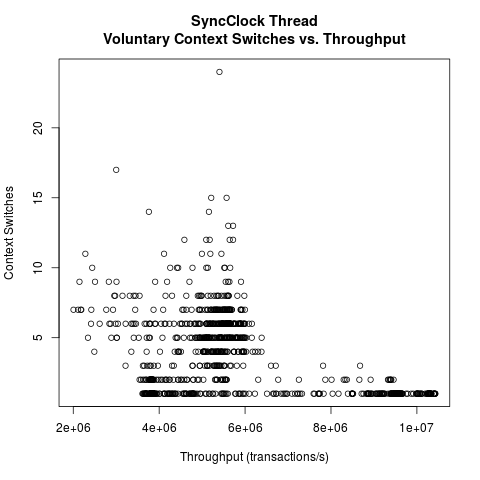
\includegraphics[height=.4\textheight]{sync_thread_throughput_context.png}
\caption{SyncClock Thread Voluntary Context Switches vs. Throughput}
\label{sync_thread_throughput_context}
\end{figure}

\begin{figure}[H]
\center
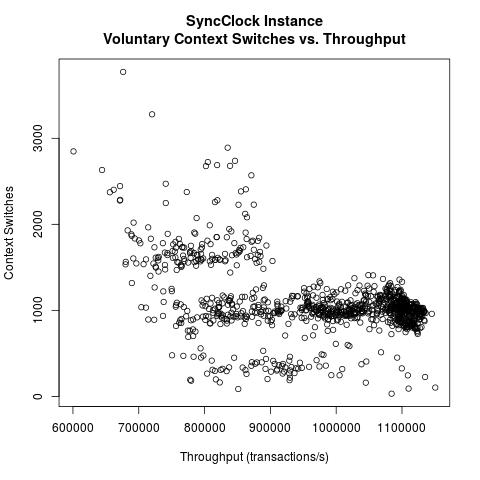
\includegraphics[height=.4\textheight]{sync_instance_throughput_context.png}
\caption{SyncClock Instance Voluntary Context Switches vs. Throughput}
\label{sync_instance_throughput_context}
\end{figure}

\begin{figure}[H]
\center
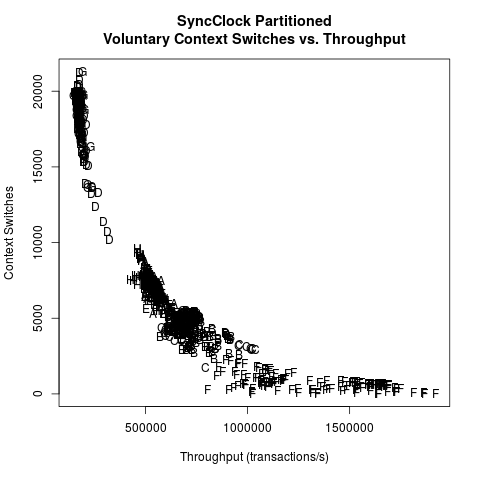
\includegraphics[height=.4\textheight]{sync_partitioned_throughput_context.png}
\caption{SyncClock Partitioned Voluntary Context Switches vs. Throughput}
\label{sync_partitioned_throughput_context}
\end{figure}

Figures~\ref{sync_thread_throughput_context}, \ref{sync_instance_throughput_context}, and \ref{sync_partitioned_throughput_context} show plots of voluntary context switches versus throughput for the Thread, Instance, and Partitioned experiments, respectively.
All show a trend where throughput increases with decreasing context switches.
Both the Thread and Instance experiments have a threshold where high throughput appears to require minimizing the number of context switches.
The plot for the Partitioned scheduler clearly shows an inverse relationship between throughput and context switches.

\begin{figure}[H]
\center
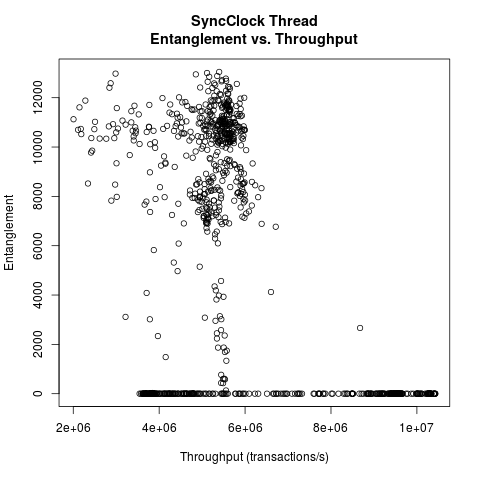
\includegraphics[height=.4\textheight]{sync_thread_throughput_entanglement.png}
\caption{SyncClock Thread Entanglement vs. Throughput}
\label{sync_thread_throughput_entanglement}
\end{figure}

\begin{figure}[H]
\center
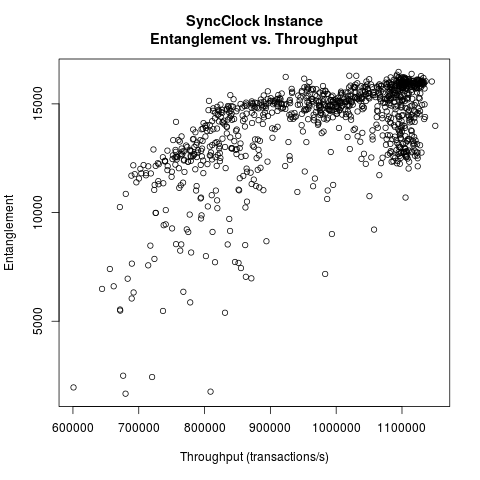
\includegraphics[height=.4\textheight]{sync_instance_throughput_entanglement.png}
\caption{SyncClock Instance Entanglement vs. Throughput}
\label{sync_instance_throughput_entanglement}
\end{figure}

\begin{figure}[H]
\center
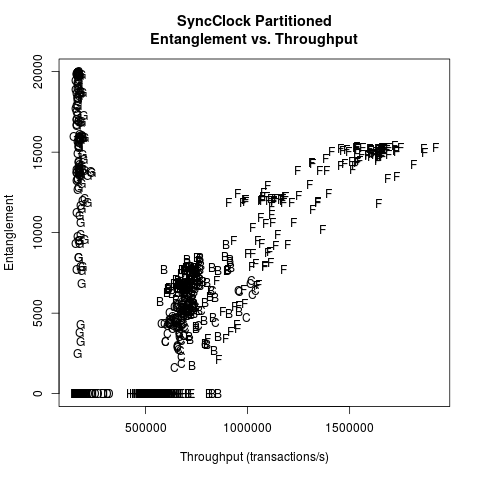
\includegraphics[height=.4\textheight]{sync_partitioned_throughput_entanglement.png}
\caption{SyncClock Partitioned Entanglement vs. Throughput}
\label{sync_partitioned_throughput_entanglement}
\end{figure}

Figures~\ref{sync_thread_throughput_entanglement}, \ref{sync_instance_throughput_entanglement}, and \ref{sync_partitioned_throughput_entanglement} show plots of entanglement versus throughput for the Thread, Instance, and Partitioned experiments, respectively.
The maximum entanglement for SyncClock is 20,000.
The plot of entanglement for the Thread scheduler resembles the plots of utilization and context switches.
The samples appear to be divided between concurrent (high entanglement, high context switch) and serial executions (low entanglement, low context switch).
For this system, it seems that it is more efficient to serialize the execution of the threads than to execute the threads concurrently and suffer context switches.

The plot of entanglement for the Instance scheduler shows a different trend where throughput increases with entanglement.
Thus, the Instance scheduler achieves high throughput when execution alternates between the threads.
The entanglement for the Partitioned scheduler appears to be a combination of three distributions.
The vertical line on the left consists of samples from the `G' partition which has maximal inter-thread conflicts and minimal opportunities for concurrent execution.
The horizontal line on the bottom (no entanglement) consists of samples from the `A', `D', `E', and `H' partitions which map Tick and Request to the same thread.
The execution is serialized with varying degrees of interference from the garbage collection actions.
The other samples contain the `B', `C', and `F' partitions which appear to show increasing throughput with entanglement.
The `F' partition has minimal inter-thread conflicts with maximal opportunities for concurrent execution.

\begin{figure}[H]
\center
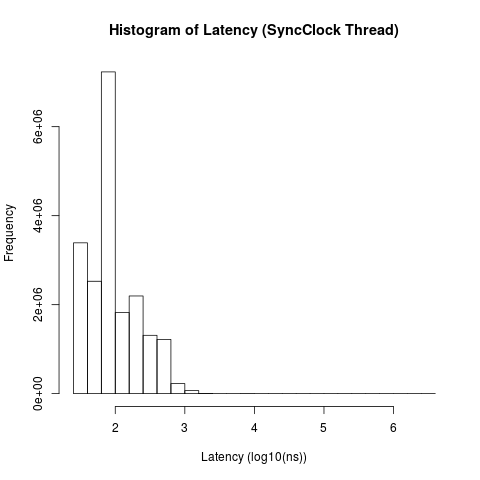
\includegraphics[height=.4\textheight]{sync_thread_latency_hist.png}
\caption{SyncClock Thread Histogram of Latency}
\label{sync_thread_latency}
\end{figure}

\begin{figure}[H]
\center
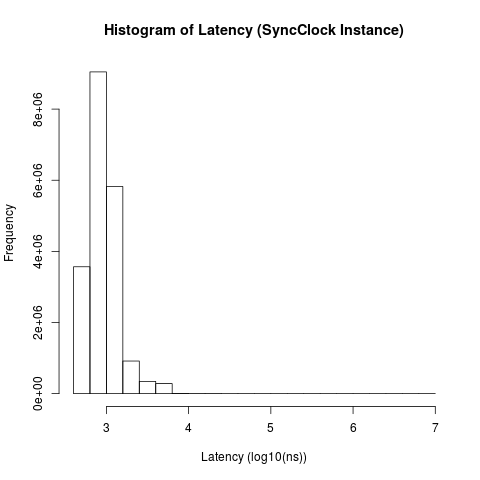
\includegraphics[height=.4\textheight]{sync_instance_latency_hist.png}
\caption{SyncClock Instance Histogram of Latency}
\label{sync_instance_latency}
\end{figure}

\begin{figure}[H]
\center
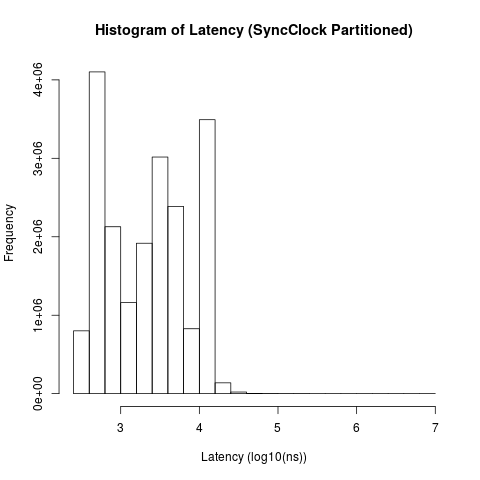
\includegraphics[height=.4\textheight]{sync_partitioned_latency_hist.png}
\caption{SyncClock Partitioned Histogram of Latency}
\label{sync_partitioned_latency}
\end{figure}

Figures~\ref{sync_thread_latency}, \ref{sync_instance_latency}, and \ref{sync_partitioned_latency} show histograms of the latency for the Thread, Instance, and Partitioned experiments, respectively.
All plots of latency use a logarithmic x-axis, as the latency distributions have very long tails.
For the Thread scheduler, the mean latency of the transactions are as follows:
\begin{center}
\begin{tabular}{cr}
Request &  72.952ns \\
Tick    & 207.145ns \\
\end{tabular}
\end{center}
The Request action does nothing more than acquire and release a lock which may explain its reduced latency.
For the Instance scheduler, the mean latency of the transactions are as follows:
\begin{center}
\begin{tabular}{cr}
Request & 1,085.32ns \\
Tick    & 1,070.57ns \\
\end{tabular}
\end{center}
For the Partitioned scheduler, the mean latency of the transactions are as follows:
\begin{center}
\begin{tabular}{cr}
Request & 4,117.71ns \\
Tick    & 4,069.06ns \\
\end{tabular}
\end{center}

\begin{figure}[H]
\center
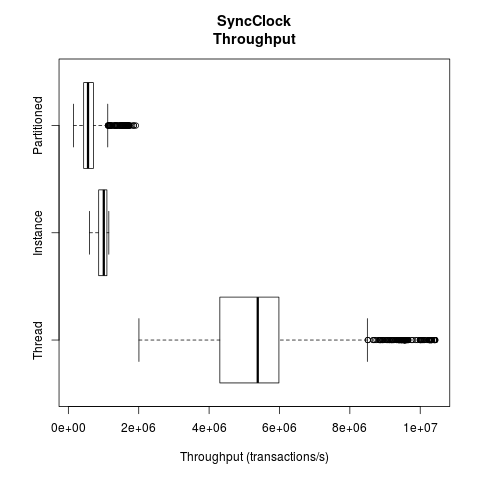
\includegraphics[height=.4\textheight]{sync_throughput_box.png}
\caption{SyncClock Throughput}
\label{sync_throughput_box}
\end{figure}

Figure~\ref{sync_throughput_box} shows a box plot of the throughput for the Thread, Instance, and Partitioned experiments.
The quantiles of the throughput in transactions/s for each scheduler are as follows:
\begin{center}
\begin{tabular}{crrrrr}
Scheduler   &       0\%   &    25\%     &    50\%     &    75\%     &   100\% \\
\hline
Partitioned &   146,788.0 &   439,051.0 &   558,954.5 &   711,073.8 &  1,919,680.0 \\
Instance    &   600,871.0 &   862,315.8 & 1,007,265.0 & 1,095,980.0 &  1,150,600.0 \\
Thread      & 2,005,940.0 & 4,308,048.0 & 5,382,440.0 & 5,983,532.0 & 10,428,200.0 \\
\end{tabular}
\end{center}
The Thread scheduler is clearly the best in terms of throughput.
The better performing partitions of the Partitioned scheduler are able to achieve the low end performance of the Thread scheduler.
In aggregate, however, the Instance scheduler appears to be better than the Partitioned scheduler.

\begin{figure}[H]
\center
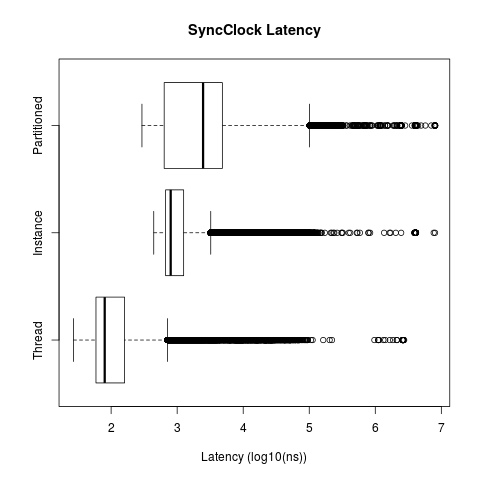
\includegraphics[height=.4\textheight]{sync_latency_box.png}
\caption{SyncClock Latency}
\label{sync_latency_box}
\end{figure}

Figure~\ref{sync_latency_box} shows a box plot of the latency for the Thread, Instance, and Partitioned experiments.
The quantiles of the latency (in ns) for each scheduler are as follows:
\begin{center}
\begin{tabular}{crrrrr}
Scheduler &       0\%  &    25\%  &    50\%  &    75\%  &   100\% \\
\hline
Partitioned & 293 &   636 & 2,469 & 4,835 &  8,100,990 \\
Instance    & 442 &   668 &   798 & 1,254 &  8,029,550 \\
Thread      &  27 &    59 &    80 &   160 &  2,736,960 \\
\end{tabular}
\end{center}
The Thread scheduler has the best latency by an order of magnitude.
This is unsurprising given the efficiency of the Thread implementation.

\section{Summary}

Perhaps the most interesting part of the implementation of the \rcgo{} run-time system is the scheduler.
Fairness, safety, and responsibility are identified as the three essential requirements for any scheduler and we illustrate how these may be accomplished in a variety of designs.
Two multi-threaded schedulers were implemented.
The Instance scheduler is based on a shared work queue of instances while the Partitioned scheduler is based on partitioning transactions among different scheduler threads.
We used throughput, latency, and utilization as metrics for evaluating schedulers for reactive components and collected data for the Instance and Partitioned schedulers by executing the AsyncClock and SyncClock systems.
The reactive component schedulers were then compared to custom implementations of the same systems using the pthreads library.
%% The results show that the reactive component schedulers are viable as event schedulers but will require improvement to become competitive with threads.
%% Moving from interpretation to compilation, reducing locking overhead, and reducing the overhead of precondition evaluation seem to be promising areas for improvement.

The AsyncClock and SyncClock experiments demonstrate both the viability of reactive components as an event system and that more work is necessary to improve the design and implementation of the run-time system.
The motivation for events was to facilitate (logical) concurrency while avoiding the overhead of context switching associated with assigning each task to a thread.
The performance of the Partitioned scheduler over the Thread implementation of AsyncClock demonstrates this idea.
As was previously mentioned, events can be combined with multi-threading but care must be taken to ensure proper synchronization.
In the reactive component model, the burden of correct synchronization is placed on the scheduler instead of the developer.

The AsyncClock system is illustrative in that it shows the advantage of events over threads but is nevertheless unrealistic as it intentionally overloads the system.
The SyncClock system represents a scenario in which there are adequate resources for each thread.
In this situation, the Instance and Partitioned schedulers perform an order of magnitude worse than the Thread implementation.
This prompts the question:  can reactive components be as efficient as threads?
While we cannot answer this question definitively, the act of converting a reactive component program to a threaded program does provide evidence that it may be possible to make reactive components as efficient as threads.
The procedure for converting a reactive component program to a threaded program involves 1) creating a reader/writer lock for each component instance, 2) creating a thread for each transaction, 3) creating a condition variable and mutex for each precondition, 4) creating a critical section for each transaction, and 5) signaling affected transactions after the critical section.
It seems feasible that this procedure can be automated.
Thus, a system of reactive components can be converted to threads or scheduled as events depending on the resources available and nature of the transactions in the system, but doing so is left for future work.

%% \section{Scheduler}

%% \paragraph{Fairness.}
%% The only requirement for a scheduler for reactive components is fairness.
%% Fairness, as applied to reactive components, means that every action receives an infinite number of opportunities to execute.

%% \paragraph{Single-threaded and multi-threaded designs.}
%% A fair single-threaded scheduler is straight-forward to implement by cycling through all the actions in a round-robin fashion.
%% Minimizing scheduling overhead by not giving opportunities to disable actions is the main optimization.
%% The same principles apply to multi-threaded schedulers with added challenge of avoiding data races.
%% That is, a multi-threaded scheduler cannot simultaneous execute two actions that may mutate the same state.
%% A multi-threaded scheduler must either prevent the various threads from selecting conflicting actions or implement a protocol that allows the threads to negotiate the conflict.
%% A scheduler might prevent conflicts by computing a schedule for each thread with explicit synchronization points.
%% The advantage of this approach is that fairness is easily enforced.
%% The drawbacks of this approach is that it is very rigid and may lead to excessive overhead and idle time waiting for synchronization.
%% Conflict can be negotiated by either selecting a different action (deferral) or blocking until there is no longer a conflict.
%% To enforce fairness, an action cannot be deferred indefinitely.
%% The remainder of the discussion focuses on the design and implementation of a multi-threaded scheduler.

%% \paragraph{Steady-state assumption.}
%% To make the design of the system tractable, we assume that the system achieves a steady-state for all executions.
%% For infinite executions, this typically involves the use of flow control/feedback to prevent producers of work from overrunning consumers of work.
%% For finite executions, the system must always achieve a \emph{fixed-point} which is a state where every action is disabled.
%% Suppose a producer task P executes on one thread and produces one work item for a consumer task C executing on another thread.
%% Furthermore, suppose that P is always enabled and is executed proportionally faster than C.
%% An infinite execution is fair, i.e., it will have and infinite number of P's and C's, however, C will never ``catch up'' to P.
%% If memory is allocated for every item produced by P, then the system will require an unbounded amount of memory.
%% In general, if a producer task that generates $n$ work items for a consumer task, then the consumer task must be executed $n$ times faster to ``keep up.''
%% The steady-state assumption means that the relative frequency of action executions is irrelevant for correctness.
%% We believe the assumption of a steady-state is not overly restrictive as all real-world systems have this property.

%% \paragraph{Motivation for a partitioned scheduler.}
%% A straightforward approach to constructing a multi-threaded scheduler is to place all actions on a global list and have each thread execute the next action on the list.
%% This organization has three potential problems.
%% First, the global list is a shared resource.
%% As the number of processors increases, so will contention on the list.
%% Second, locking is mandatory to avoid data races.
%% To execute an action, a thread must acquire a lock for all instances involved in the action.
%% Third, this approach requires extra logic for good cache behavior.
%% A thread may not want the next action on the list if the action has no affinity for the thread.

%% In a partitioned scheduler, the actions are partitioned among the available threads.
%% This organization eliminates contention over a shared global list and has the potential for good cache behavior.
%% Data races can be avoided through partitioning and locking.

\chapter{Conclusions and Future Work}
\label{conclusion}

A reactive system is characterized by ``ongoing interactions with its environment''~\cite{manna1992temporal}.
Asynchronous concurrency is a feature of reactive systems that makes them inherently difficult to develop.
Reactive systems are already used in various forms of critical infrastructure and the number, diversity, and scale of reactive systems is expected to increase given the continuing proliferation of embedded, networked, and interactive systems.
Decomposition and composition are two complementary techniques that are helpful when designing and implementing reactive systems, especially given such increases in complexity.
We argue that the dominant techniques based on multiple sequential threads/processes thwart decomposition and composition and thus contribute to the accidental complexity associated with reactive system development.

Specifically, we believe that a model for reactive systems should facilitate \emph{principled} composition and decomposition.
Beyond defining units of composition and a means of composition, a model for reactive systems should facilitate practical techniques like recursive encapsulation and behavior abstraction through interfaces.
Composition should be compositional meaning that the properties of a unit of composition can be stated in terms of the properties of its constituent units of composition.
Finally, units of composition should be subject to substitutional equivalence meaning that the definition of a unit of composition can be substituted for its use and vice versa.
Substitutional equivalence allows a complex system to be reduced to a single unit and a complex unit to be decomposed into a system of simpler units.

In Chapter~\ref{model}, we presented the \emph{reactive component} model for reactive systems.
The reactive component model is based on models like UNITY and I/O Automata in that computation is carried out via a sequence of atomic state transitions selected non-deterministically.
To these models, reactive components adds facilities for recursive encapsulation and interfaces that facilitate third-party composition via explicit binding.
A reactive component is a set of state variables, atomic state transitions, and ports.
The state variables of a reactive component may only be updated by the transitions associated with that component to ensure compositionality.
Ports have passive and active sides.
Push ports allow a transition in a component to synchronously induce a transition in another component while pull ports allow components to export and access values and state.
An action is a transition with a precondition that can be executed by the scheduler.
A reaction is a passive push port and transition that can be linked to an active push port to form an atomic transition that spans multiple components.
A getter is a passive pull port and an expression that allows the state of a component to be accessed in a safe way.
A transition is divided into two phases called the immutable phase and the mutable phase.
Components may not change state in the immutable phase, which allows their state to be shared via temporary values.
State is updated from the temporary values in the mutable phase of a transition.
This division facilitates the composition of transitions in a principled way as it provides a clear interpretation of the state of a component before and after a transition.
This, in turn, allows the properties derived from the state variables and transitions in one component to be linked to the properties of other components to facilitate compositional reasoning.

The interface-based composition semantics of reactive components introduces the possibility of non-deterministic transitions.
A non-deterministic state transition occurs when a state variable is updated in disparate ways in different sub-transitions.
The detection of non-deterministic state transitions arising from composition is generally undecidable.
However, allowing a reactive component instance to serve as a proxy for its state variables reduces the problem of detecting non-deterministic transitions to simple graph and set theoretic problems.

Practicality was one of our goals when designing the reactive component model.
That is, we intended it to be implemented and used to design and build real-world systems in an effort to reduce the accidental complexity associated with reasoning about a system using one set of semantics and implementing it using another.
Thus, we presented the \rcgo{} programming language for reactive components in Chapter~\ref{language}.
We adopted the Go programming language as the basis for \rcgo{} and added syntax and semantics to support the elements of the reactive component model.
The major challenge when designing the language was supporting reference and move semantics while preserving the isolation of state between reactive components.
Reference semantics are important as they allow the construction of arbitrary linked data structures and move semantics are important for efficient communication between reactive components.
Supporting these features required techniques from race-free programming languages.
Thus, we added intrinsic and indirection mutability attributes to pointer types.
Immutable indirection mutability is used to enforce the immutable phase of state transitions while foreign indirection mutability prevents pointers referring to a component's state from being saved by another component.
To facilitate move semantics, we introduced a transferrable heap type which facilitates the construction and transfer of self-contained linked data structures.

Chapter~\ref{implementation} described the implementation of key features for the \rcgo{} run-time system.
The two major assumptions leveraged throughout the design of the run-time system are 1) components instances serve as a proxy for their state variables and 2)~the reactive systems being implemented are static meaning that the number and configuration of the reactive components in the system are fixed.
With these two assumptions we present an algorithm that checks for sound composition.
The algorithm treats each transaction, i.e., a composed transition, as a graph with nodes corresponding to actions, reactions, activate statements, and push ports.
This algorithm checks for non-deterministic transactions by ensuring that the graph contains no cycles and that a component instance participates in at most one non-empty activate statement.

The execution of a transaction requires two passes over a transaction graph corresponding to the immutable phase and mutable phase.
The main challenge when computing the immutable phase is recording the context of each action/reaction that executes an activate statement so that its continuation may be executed in the mutable phase.
To accomplish this, we created the novel \emph{synchronized two-phase calling convention} which captures the context of an activate statement using an ordinary call stack.
The significance of this approach is that transactions can be executed efficiently without allocating a stack frame on the heap.

The interpreter for \rcgo{} uses garbage collection to reclaim memory.
Garbage collection avoids dangling pointers which could threaten the isolation of state among component instances.
All component state in \rcgo{} may be attributed to exactly one reactive component instance.
This admits an embarrassingly parallel garbage collection algorithm, as garbage collection can be performed on each component in parallel.

The schedulers described in Chapter~\ref{scheduler} are the most significant parts of the \rcgo{} implementation.
A scheduler has the responsibility of executing transactions with fairness.
The challenge when designing and implementing a scheduler is to convert the logically serial execution of the reactive component model to physically concurrent execution.
To do this, the scheduler utilizes the composition analysis to determine which transactions may be executed in parallel.
We present two scheduler implementations:  one is based on a globally shared work queue while the other is based on a static partitioning of the transactions.
To evaluate the scheduler, we simulate a number of rounds in a simple request-response protocol.
In the first design, the \rcgo{} schedulers outperform a custom multi-threaded implementation due to excessive context switching in the multi-threaded program.
This suggests that reactive components are viable as a concurrent event-based approach to reactive systems.
The request-response protocol was then rewritten to be more conducive to the test hardware.
The results of this experiment show that additional work is required to raise the performance of the \rcgo{} interpreter to be on par with optimized libraries for multi-threading.

\section{Conclusions}

The reactive component model is viable for designing and implementing reactive systems.
The main goal of this work is to reduce the accidental complexity associated with the design and implementation of reactive systems.
We believe the source of this accidental complexity is the mismatch between the semantics of reactive systems and the sequential multi-threaded techniques used to implement them.
Furthermore, we observe that sequential multi-threaded techniques fail to adequately manage complexity in the face of composition and decomposition.
There are three main ideas in the reactive component model that make it a viable solution to these problems.
First, the reactive component model addresses the semantics of reactive systems by interpreting computation in reactive systems as a non-deterministic sequence of atomic events which have the added benefit of composing well.
Second, the reactive component model uses encapsulation to guarantee compositionality.
The state of each reactive component instance may only be manipulated by the transitions of that component and therefore properties established from the transitions may never be violated through subsequent composition.
This principle extends to constellations of interacting (composed) components that are themselves encapsulated.
Third, compound state transitions spanning multiple components are formed using parallel composition instead of sequential composition.
Parallel composition as expressed through the immutable phase and mutable phase concepts in the reactive component model provides a clear interpretation of compound atomic transactions.

The semantics of reactive components can be checked efficiently.
The three main checks are 1)~the enforcement of immutability during the immutable phase, 2) prevention of shared state, and 3) the detection of non-deterministic transitions.
The first two properties are enforced through the type system and type checking algorithm.
The detection of non-deterministic state transitions can only be performed once the set of concrete instances is known.
The current algorithm leverages the static system assumption to create concrete transactions from compound transitions.
These transactions can be checked in polynomial time.
The key point is that the reactive component model does not rest on assumptions that cannot be realized in practice, as all of these algorithms have been implemented.

There is evidence that a run-time system for reactive components could be made efficient enough to compete with optimized multi-threaded approaches.
A common approach to implementing high-performance reactive systems is to use a number of concurrent event loops which maximizes the use of available cores while minimizing context switches.
The scheduler implementations in Chapter~\ref{scheduler} are examples of this kind of design.
The efficacy of this approach is seen in the first experiment where the reactive component schedulers outperform a multi-threaded implementation due to context switching.
The second experiment demonstrates that additional work is necessary to improve the performance of the reactive component schedulers to make them comparable to custom multi-threaded implementations.

\section{Future Work}

This dissertation has presented the reactive component model as an alternative to sequential threads for designing and implementing reactive systems.
As a model, sequential thread-based computation is firmly entrenched in many areas including hardware (synchronous sequential processors), operating systems (process and thread abstractions), and programming languages.
Thus, we may consider possibilities such as hardware architectures specifically designed for reactive components and operating systems where the main abstraction is the reactive component or transaction instead of the thread.
These topics are quite ambitious and additional work is required before these topics may be adequately addressed.
First, we must generalize the reactive component model for dynamic systems (Section~\ref{dynamic_systems}).
This is necessary as an operating system must be able to load and configure reactive components and many reactive applications are naturally formulated using dynamic configurations.
Second, we must consider the problem of scheduling transactions, as the scheduler will have a significant impact on the performance of reactive component applications (Section~\ref{future_scheduler}).

\subsection{Dynamic Systems}
\label{dynamic_systems}
Two assumptions were necessary to make the analysis of systems of reactive components tractable.
First, we assume that a reactive component instance is a proxy for its state variables.
Pull ports and getters reduce the impact of this assumption as a designer can decompose at will which yields more component instances for fine-grained analysis.
Second, we assume that a reactive system has a fixed number of component instances in a fixed configuration.
While we argue that many systems of interest have this property, removing or weakening this assumption would make the reactive component more general and more applicable to areas like enterprise level distributed systems and cloud computing.

The first level of support with regards to dynamic systems is adding support for dynamic sets of components and bindings.
To illustrate, consider how the implementation of a TCP or UDP stack could use a dynamic array or set of components.
The various ports in TCP/UDP represent independent data flows that may be processed in parallel.
To exploit this parallelism in the reactive component model, each port should be processed by a unique reactive component instance.
It is theoretically possible to declare a component instance for the 65,536 ports defined in the protocol.
However, doing so in practice would be wasteful as only a subset of ports are active at any given time.
Thus, we require the ability to dynamically allocate and bind component instances.

Models like UNITY and I/O Automata use parameterized models to reason about systems consisting of an arbitrary number of program instances.
For the TCP/UDP port example, these models would assume that all 65,536 ports exist and are sent activate and deactivate messages as necessary.
From an implementation perspective, it may be possible to use this idea and automatically allocate and deallocate resources for component instances when they receive activate and deactivate messages.

Providing support for dynamic sets of components and bindings requires further extensions to the model, language, and implementation.
The major extensions to the model would include adding support for dynamic arrays or sets of components and parameterized bindings that allow a component to interact with a dynamically allocated component.
The next step then would be mapping the extended semantics into the \rcgo{} programming language.
Supporting dynamically allocated components and bindings in the implementation also would require extending the check for sound composition and providing run-time support for the features in the language.
Checking for sound composition in a system with dynamic sets of components would require the run-time system to perform an inductive proof over all sets of dynamic components in the system.
That is, the run-time system must prove that all transactions remain deterministic when any set of components increases in size.

The dynamic sets of components and bindings described so far are subject to static analysis as the dimensions of variability are expressed in the code.
The next level of support would involved unplanned variability where new component types and instances are loaded and bound.
Supporting this level of dynamism requires support for programmatic loading and binding including a service discovery mechanism that allows components to publish their existence and other components to find them.
In terms of enforcing the reactive component model, the check for sound composition must be performed at runtime and constitutes a form of admission control.
Thus, additional work is needed to determine if the sound composition check can be modified for use in an on-line setting or if additional restrictions must be placed on the model to ensure an efficient on-line check.

\subsection{Scheduling}
\label{future_scheduler}

There are three main areas that may be addressed to improve the performance of the Instance and Partitioned schedulers.
First, we may attempt to improve the efficiency of the schedulers through better design and implementation.
The evaluation in Chapter~\ref{scheduler} can serve as a basis for future improvements.
Second, we may attempt to reduce the overhead of the Linux scheduler.
In Linux, the threads made available via the pthreads library are scheduled by the Linux kernel.
The Instance and Partitioned schedulers, then, are themselves scheduled by the Linux kernel.
Thus, it may be necessary to implement a scheduler for reactive components at the kernel level to restrict this source of overhead.
Third, we may move from interpretation to compilation.
To test this idea, we timed a loop to sum the numbers in the range [0, 1,000,000) and averaged it over 1,000 runs for a C++ implementation and a reactive component implementation.
The average time for the reactive component implementation was 0.1304896 seconds and the average time for the C++ implementation was 0.0009984909 seconds; a speed-up factor of 131.
This is very much a ``back of the envelope'' calculation; the actual improvement in moving from interpretation to compilation may be less than this.

We selected the AsyncClock and SyncClock systems to evaluate the schedulers because they are small enough to understand but complex enough to show interesting behavior.
The actual computation performed by these systems is minimal, i.e., setting Boolean flags and incrementing counters.
Most likely, these operations can be performed in a single clock cycle (for compiled programs).
One obvious direction for future work, then, is to experiment with complex transactions and varied workloads.
However, it is important to consider the possibility that real workloads will contain computationally simple transactions such as those found in the clock systems.
Furthermore, one of the motivations for decomposing systems is to break up complex systems into smaller, reusable, and easier to understand systems.
The results in Chapter~\ref{scheduler} demonstrate the diminishing return where the transactions become so simple that execution is dominated by overhead, i.e., it is more efficient to serialize execution than execute actions in parallel.
Simple transactions are a foreseeable consequence of decomposition and designers should not be penalized for decomposing complex systems.
Thus, one of the goals of scheduler design is to push the horizon of the diminishing return as far as possible.
When coupled with responsiveness, the desired property in a scheduler is one whose throughput does not diminish with entanglement.

One goal for a reactive component scheduler may be to optimize the evaluation of preconditions.
Two possible goals are to reduce the number of times a precondition is evaluated (lazy vs. eager) or to reduce the overhead of evaluating a single precondition.
The reactive component model allows arbitrary Boolean expressions to be used as preconditions.
One idea may be to eliminate preconditions and replace them with explicit scheduling instructions, but this may become tedious and error prone.
A compromise solution may involve restricting the complexity of preconditions to simple Boolean expressions, i.e., with no function calls.
With this restriction, it may become possible to determine which activate statements enable/disable a transaction.

To be safe, all concurrent schedulers require synchronization to protect the mutable state in a transaction.
The approach taken by the oblivious Instance and Partitioned schedulers is to acquire locks protecting the state of each involved component before executing a transaction.
The Partitioned scheduler demonstrates how asynchronous locking can be used to create a work-conserving scheduler.
As indicated by the results in Chapter~\ref{scheduler}, a major challenge is to make synchronization as efficient as possible.

Another direction for future work is to explore options that accomplish synchronization without locking or with minimal locking.
Partitioning combined with non-preemption may create opportunities to synchronize without locking.
Let $u$ be a transaction assigned to a specific scheduler thread and let $I$ be the set of instances involved in $u$.
Furthermore, let all transactions involving any component in $I$ be mapped to the same scheduler thread (the single-threaded schedulers described in Chapter~\ref{scheduler} do this by virtue of their design).
In this scenario, no locks are needed for a safe execution of $u$ because all other transactions that could change the relevant component state are excluded from executing due to the non-preemptive nature of the scheduler.
This phenomenon is illustrated graphically by coloring the nodes in a race graph according to the thread to which they have been assigned.
A transaction whose immediate neighbors all share the same color as the transaction itself can execute without acquiring locks.
This suggests that algorithms that detect clusters of transactions in the race graph may be used to optimize the assignment of transactions to scheduler threads.

Locking also may be optimized by performing operations on the race graph.
For example, adjacent transactions in the race graph can be merged and executed under the same set of locks.
This procedure can be used to create complex transactions that amortize the locking overhead.
Most likely, the merging algorithm would make use of some heuristic that measures the perceived benefit of merging the transactions.
For example, the edges in the race graph could be weighted with the Jacquard Index of the instance sets, i.e., the edges are weighted with a score indicating that the set of locks are similar.
The merging algorithm must balance the goal of simplifying the locking with the goal of exploiting concurrency.
For example, merging the Request and Response transactions eliminates the potential concurrency between the Request and Tick transactions in the \emph{AsyncClock} system.

Similarity between instance sets suggests that locks may be eliminated by combining them.
To illustrate, the \emph{AsyncClock} system contains three locks corresponding to the three components.
Suppose that the same lock is used to protect both the Client and the Server.
This reduces the number of locks needed to execute the Request transaction from two to one and the number of locks needed to execute the Response transaction from three to two.

The challenges associated with locking invite us to step back and consider the fundamental aspects of the problem that necessitate a locking protocol.
The scheduler designs put forth so far are distributed in the sense that each scheduler thread is making an independent decision about the next transaction to execute.
Locking is the means by which the scheduler thread discovers the decisions made by the other scheduler threads to determine if the transaction under consideration is compatible with the transactions already chosen by the other threads.
The locking protocol becomes unnecessary if the decisions made by the other threads are already available, i.e., a knowledgeable scheduler.
This suggests that orchestration may be used to ensure safety in a multi-threaded scheduler without locking.
In this model, a manager thread assigns transactions to scheduler threads who execute the transactions without acquiring locks.
The primary job of the manager thread is to enforce safety by only allowing the concurrent execution of disconnected transactions in the race graph.
This approach may make use of a dedicated manager thread (Producer-Consumer) or use the Leader-Follower pattern~\cite{schmidt2000pattern}.
An efficient implementation of the scheduler state, especially if it is shared through the Leader-Follower pattern, is a concern for this kind of scheduler.
For systems with a fixed set of transactions, a compiler may be able to generate a scheduling automaton by enumerating the scheduler states $S$, pruning unsafe states and transitions according the rules outlined in Section~\ref{scheduling_problem}, pruning transitions to ensure fairness, etc.
This formulation also may have the advantage of yielding compact scheduler state.

Cache awareness and migration are two concerns that reactive component schedulers share with thread schedulers.
Cache awareness attempts to improve the performance of a system by scheduling a computation on the same processor core because the state required for the computation may already be available in the cache.
Thus, a reactive component scheduler may attempt to create an affinity between a transaction and a scheduler thread or processor core.
Partitioning on the basis of shared component state satisfies this implicitly.
Migration reassigns a computation to a different core to balance the load among the cores or free a core so that it may be shut down.
The challenge with respect to migration is to define load imbalance in a meaningful way.
The migration algorithm will most likely be expressed as an optimization problem that attempts to find a global optimum for the throughput and latency of each action.

Another design dimension for a reactive component scheduler is preemption.
The main use of preemption is to share a physical core among many computations that are ready to execute.
A reactive component scheduler may wish to preempt a long-running transaction to execute other enabled transactions.
A preemptive scheduler for reactive components can take advantage of existing work on thread preemption.

%% POSIX environment, possibly bare metal

%% \item termination
%% \item active - terminating - idling (most servers have 10\% utilization)
%% \item flow control
%% \item always enabled actions
%% \item reactive components in hardware
%% \item long running actions

%% Another assumption we made when designing the language and run-time system was the use of garbage collection.
%% For our purposes, garbage collection helps enforce the isolation of state between components by preventing dangling pointers.
%% The independence of each component instance admitted a simple parallel garbage collection algorithm as garbage collection can be performed for each instance in parallel.
%% The obvious alternative to garbage collection is automatic reference counting and existing work as represented by the Rust programming language indicates that this approach may be feasible even for low-level systems programming.
%% Thus, one area exploration may be to use referencing counting in lieu of garbage collection.

%% The language \rcgo{} is based on the Go programming language.
%% One are for future work is to consider other base languages like C, C++, Java, Rust, Python, etc.

\section{Broader Impacts}

Reactive systems have had a profound impact on society and will continue to impact society for the foreseeable future.
Some reactive systems like the Internet and smart phones have high visibility while others, like the army of micro-controllers present in a modern automobile or a home appliance, are less conspicuous but nevertheless help us with our daily activities and contribute to our safety and comfort.
Some reactive systems, like pace makers, life support machines, and robotic surgical instruments, even have a direct impact on our health and well being.
The goal of this research is to ensure the quality and reliability of reactive systems in the face of predicted increases in size, diversity, and complexity.

%% \paragraph{Contributions.}
%% In this work, we propose three contributions to the state of the art in reactive systems development.
%% First, we propose a new model called reactive components for reactive systems based on direct support for reactive semantics and principled composition and decomposition.
%% A reactive component is a set of state variables and non-deterministically scheduled atomic transitions.
%% Transitions in different components can be linked via ports which also allow data to be exchanged among components.
%% Implicit atomicity and non-deterministic sequencing allow reactive systems to be designed and implemented through principled decomposition and composition.

%% Second, we propose to implement the model of reactive components to determine whether the assumptions and semantics of the model can be realized using existing techniques and architectures.
%% For tractability, we limit the implementation to systems with a fixed configuration of reactive components.
%% The major challenge when implementing the model is to enforce the semantics that require all state transitions to be deterministic.
%% Our approach is based on the encoding of transitions using a pure functional or applicative language which in turn requires an approach to data structures (persistent vs. ephemeral).
%% The platform will consist of a compiler for a high-level language shaped by the semantics of reactive components and a virtual machine.

%% Third, we propose to evaluate the model of reactive components and its implementation.
%% In the first part of the evaluation, we will apply the model to the design and development of an embedded web server.
%% The goal of the evaluation is to gauge the fitness of the model and usefulness of principled composition and decomposition by applying the model to a representative real-world reactive system.
%% Developing an embedded web server allows the model to be applied to a number of problems in reactive systems such as hardware, network protocols, and interactive applications.
%% The second part of the evaluation is a quantitative measurement of the implementation (compiler and virtual machine) to ensure that the employed algorithms and techniques result in a practical engineering tool.

%%\paragraph{Future work.}
%% \paragraph{Beyond this dissertation.}
%% While we argue that the static system assumption is valid, it is nevertheless restrictive and prevents designs that may be more naturally formulated using a unbound number of components.
%% Thus, we believe the first step to applying reactive components to a broader range of systems is an extension to dynamic systems.
%% Another barrier to the wide-spread adoption of reactive systems is its reliance on a virtual machine.
%% As indicated by the Java programming language, a virtual machine is appropriate for application level programming while lower-level programming is often performed in a compiled language such as C.
%% Thus, the compiler proposed in section~\ref{implementation} may serve as the beginning for a compiler capable of emitting machine code.
%% The main direction for future work is to continue to gain experience with reactive components by implementing systems.
%% The class of reactive systems is enormous and spans everything from the programs that control 8-bit micro-controllers to the distributed applications running Google's cluster.
%% We believe the evaluation of section~\ref{evaluation} is an appropriate first case study but necessarily lacks the depth and breadth needed to fully evaluate reactive components.

%% \paragraph{Outcomes.}
%% The proposed research will be successful if it generates new knowledge regarding the design and implementation of reactive systems.
%% The conclusion of this research will be a explanation as to whether or not reactive components are a viable approach to reactive systems and if so, what additional research is warranted.
%% If the research concludes that reactive components are not a viable approach, it will reveal the characteristics of reactive components and more generally models based on the non-deterministic sequencing and implicit atomicity that make them an inappropriate or impractical foundation for reactive systems.
%% If reactive components are indeed a viable approach to reactive systems, then the proposed work could represent the beginning of a significant shift in the theory and practice concerning reactive systems.
%% That is, reactive components have the potential to replace threads and events which are the dominant approaches to reactive system development today.


\appendix

\chapter{Partition Tables}
\label{partition_tables}

\begin{longtable}{ccccccccr}
Symbol & System & Server & Counter & Client & Response & Tick & Request & Count \\
\hline
\endhead
A & 0 & 0 & 0 & 0 & 0 & 0 & 0 & 17 \\
B & 0 & 0 & 0 & 0 & 0 & 0 & 1 & 16 \\
C & 0 & 0 & 0 & 0 & 0 & 1 & 0 & 20 \\
D & 0 & 0 & 0 & 0 & 0 & 1 & 1 & 12 \\
E & 0 & 0 & 0 & 0 & 1 & 0 & 0 & 11 \\
F & 0 & 0 & 0 & 0 & 1 & 0 & 1 & 17 \\
G & 0 & 0 & 0 & 0 & 1 & 1 & 0 & 11 \\
H & 0 & 0 & 0 & 0 & 1 & 1 & 1 & 12 \\
I & 0 & 0 & 0 & 1 & 0 & 0 & 0 & 13 \\
J & 0 & 0 & 0 & 1 & 0 & 0 & 1 & 6 \\
K & 0 & 0 & 0 & 1 & 0 & 1 & 0 & 17 \\
L & 0 & 0 & 0 & 1 & 0 & 1 & 1 & 20 \\
M & 0 & 0 & 0 & 1 & 1 & 0 & 0 & 16 \\
N & 0 & 0 & 0 & 1 & 1 & 0 & 1 & 25 \\
O & 0 & 0 & 0 & 1 & 1 & 1 & 0 & 14 \\
P & 0 & 0 & 0 & 1 & 1 & 1 & 1 & 12 \\
Q & 0 & 0 & 1 & 0 & 0 & 0 & 0 & 14 \\
R & 0 & 0 & 1 & 0 & 0 & 0 & 1 & 11 \\
S & 0 & 0 & 1 & 0 & 0 & 1 & 0 & 9 \\
T & 0 & 0 & 1 & 0 & 0 & 1 & 1 & 15 \\
U & 0 & 0 & 1 & 0 & 1 & 0 & 0 & 20 \\
V & 0 & 0 & 1 & 0 & 1 & 0 & 1 & 12 \\
W & 0 & 0 & 1 & 0 & 1 & 1 & 0 & 18 \\
X & 0 & 0 & 1 & 0 & 1 & 1 & 1 & 16 \\
Y & 0 & 0 & 1 & 1 & 0 & 0 & 0 & 16 \\
Z & 0 & 0 & 1 & 1 & 0 & 0 & 1 & 16 \\
a & 0 & 0 & 1 & 1 & 0 & 1 & 0 & 18 \\
b & 0 & 0 & 1 & 1 & 0 & 1 & 1 & 21 \\
c & 0 & 0 & 1 & 1 & 1 & 0 & 0 & 16 \\
d & 0 & 0 & 1 & 1 & 1 & 0 & 1 & 9 \\
e & 0 & 0 & 1 & 1 & 1 & 1 & 0 & 14 \\
f & 0 & 0 & 1 & 1 & 1 & 1 & 1 & 11 \\
g & 0 & 1 & 0 & 0 & 0 & 0 & 0 & 16 \\
h & 0 & 1 & 0 & 0 & 0 & 0 & 1 & 17 \\
i & 0 & 1 & 0 & 0 & 0 & 1 & 0 & 12 \\
j & 0 & 1 & 0 & 0 & 0 & 1 & 1 & 20 \\
k & 0 & 1 & 0 & 0 & 1 & 0 & 0 & 16 \\
l & 0 & 1 & 0 & 0 & 1 & 0 & 1 & 16 \\
m & 0 & 1 & 0 & 0 & 1 & 1 & 0 & 13 \\
n & 0 & 1 & 0 & 0 & 1 & 1 & 1 & 17 \\
o & 0 & 1 & 0 & 1 & 0 & 0 & 0 & 25 \\
p & 0 & 1 & 0 & 1 & 0 & 0 & 1 & 22 \\
q & 0 & 1 & 0 & 1 & 0 & 1 & 0 & 13 \\
r & 0 & 1 & 0 & 1 & 0 & 1 & 1 & 14 \\
s & 0 & 1 & 0 & 1 & 1 & 0 & 0 & 10 \\
t & 0 & 1 & 0 & 1 & 1 & 0 & 1 & 11 \\
u & 0 & 1 & 0 & 1 & 1 & 1 & 0 & 27 \\
v & 0 & 1 & 0 & 1 & 1 & 1 & 1 & 16 \\
w & 0 & 1 & 1 & 0 & 0 & 0 & 0 & 12 \\
x & 0 & 1 & 1 & 0 & 0 & 0 & 1 & 18 \\
y & 0 & 1 & 1 & 0 & 0 & 1 & 0 & 17 \\
z & 0 & 1 & 1 & 0 & 0 & 1 & 1 & 12 \\
0 & 0 & 1 & 1 & 0 & 1 & 0 & 0 & 17 \\
1 & 0 & 1 & 1 & 0 & 1 & 0 & 1 & 7 \\
2 & 0 & 1 & 1 & 0 & 1 & 1 & 0 & 11 \\
3 & 0 & 1 & 1 & 0 & 1 & 1 & 1 & 17 \\
4 & 0 & 1 & 1 & 1 & 0 & 0 & 0 & 19 \\
5 & 0 & 1 & 1 & 1 & 0 & 0 & 1 & 19 \\
6 & 0 & 1 & 1 & 1 & 0 & 1 & 0 & 16 \\
7 & 0 & 1 & 1 & 1 & 0 & 1 & 1 & 17 \\
8 & 0 & 1 & 1 & 1 & 1 & 0 & 0 & 21 \\
9 & 0 & 1 & 1 & 1 & 1 & 0 & 1 & 22 \\
@ & 0 & 1 & 1 & 1 & 1 & 1 & 0 & 22 \\
\$ & 0 & 1 & 1 & 1 & 1 & 1 & 1 & 13 \\

\caption[Partitions for the AsyncClock system]{Partitions for the AsyncClock system.  The Symbol column contains the symbol used to represent this partition on plots.  The System, Server, Counter, and Client columns indicate the thread used for the garbage collection action for the respective component.  The Response, Tick, and Request columns indicate the thread used for the respective transaction.  The Count column indicates the number of samples for this partition.}
\label{async_partitions}
\end{longtable}

\begin{longtable}{ccccccccr}
Symbol & System & Counter & Request & Tick & Count \\
\hline
\endhead
A & 0 & 0 & 0 & 0 & 117 \\
B & 0 & 0 & 0 & 1 & 137 \\
C & 0 & 0 & 1 & 0 & 119 \\
D & 0 & 0 & 1 & 1 & 114 \\
E & 0 & 1 & 0 & 0 & 117 \\
F & 0 & 1 & 0 & 1 & 140 \\
G & 0 & 1 & 1 & 0 & 135 \\
H & 0 & 1 & 1 & 1 & 121 \\

\caption[Partitions for the SyncClock system]{Partitions for the SyncClock system.  The Symbol column contains the symbol used to represent this partition on plots.  The System and Counter columns indicate the thread used for the garbage collection action for the respective component.  The Request and Tick columns indicate the thread used for the respective transaction.  The Count column indicates the number of samples for this partition.}
\label{sync_partitions}
\end{longtable}

\bibliographystyle{plain}
\begin{spacing}{1.0}
\bibliography{paper}{}
\end{spacing}
\nocite{*}

\begin{thesisauthorvita}
%
% This is just a sample of what to do in a vita
%
\begin{center}
{\large\thesisauthor}
\end{center}
%
% Need to 'fold' long labels
%
\newcommand{\vitalabel}[1]%
  {\raisebox{0pt}[1ex][0pt]
    {\makebox[\labelwidth][l]%
      {\parbox[t]{\labelwidth}{\hspace{0pt}\textbf{#1}}}}}
%
% Here's the list definition
%
\begin{list}
  {}%                                        nodefault label
  { \renewcommand{\makelabel}{\vitalabel}%   setting labels
    \setlength{\labelwidth}{100pt}%          label width
    \setlength{\leftmargin}{120pt}%
    \setlength{\itemindent}{0pt}%            don't indent first line of items
    \setlength{\parsep}{\baselineskip}%               space between paragraphs
    \setlength{\itemsep}{5pt}%               additional space between items
    }

\item[Degrees] B.S.\ Summa Cum Laude, Electrical Engineering, December 2006 \\
               B.S.\ Summa Cum Laude, Computer Engineering, December 2006 \\
               Ph.D. Computer Science, December 2016
%% \item[Professional\linebreak Societies]
%%   Association for Computing Machines \\
%%   The Touring Society \\
%%   The Free Software Foundation
\item[Publications]
  Wilson, J., Dai, M., Jakupovic, E., Watson, S., \& Meng, F. (2007). Supercomputing with toys: harnessing the power of NVIDIA 8800GTX and playstation 3 for bioinformatics problems. In \textit{Computational Systems Bioinformatics Conference} (Vol. 6, pp. 387-390).

  Thomas, L., Wilson, J., Roman, G. C., \& Gill, C. (2009, November). Achieving coordination through dynamic construction of open workflows. In \textit{ACM/IFIP/USENIX International Conference on Distributed Systems Platforms and Open Distributed Processing} (pp. 268-287). Springer Berlin Heidelberg.

  Xi, S., Wilson, J., Lu, C., \& Gill, C. (2011, October). RT-Xen: towards real-time hypervisor scheduling in xen. In \textit{IEEE International Conference on Embedded Software (EMSOFT)} (pp. 39-48).
\end{list}
\flushright
\thesismonth\ \thesisyear
\end{thesisauthorvita}

%% \begin{thesisshorttitlepage}
%% %\iffalse
%% {\small

%% \textbf{NOTE:}	This is a sample of a ``short title'' page.  Please change the
%% line above to use an appropriate ``short title'' for your thesis, insert your
%% last name, and include your degree and year in which the degree will be earned.
%% Separate elements using commas, as illustrated in the sample above.
%% \uline{Your ``short title'' cannot exceed 35 characters, counting spaces}.  It
%% does not matter if there is a page number at the bottom of the page.

%% \textbf{IMPORTANT:} This page should be printed and taped securely to each of
%% the three manila envelopes used to submit your final hard copies.  Remove this
%% page before submitting your final copies (i.e., this page should not be
%% included in either your electronic submission or your hard copy submissions).
%% See Appendix~\ref{app:procedures} for further details if necessary.
%% }
%% %\fi
%% \end{thesisshorttitlepage}

\end{document}
